\subsection{Kinematic Distributions}
\label{sec:kinedistri}

\subsubsection{\texorpdfstring{Kinematic Distributions of $\pi^0$}{Kinematic Distributions of pi0}}
\label{sec:kinedistri_pi0}

\begin{figure}[H]
\captionsetup[subfloat]{farskip=2pt,captionskip=1pt}
\centering
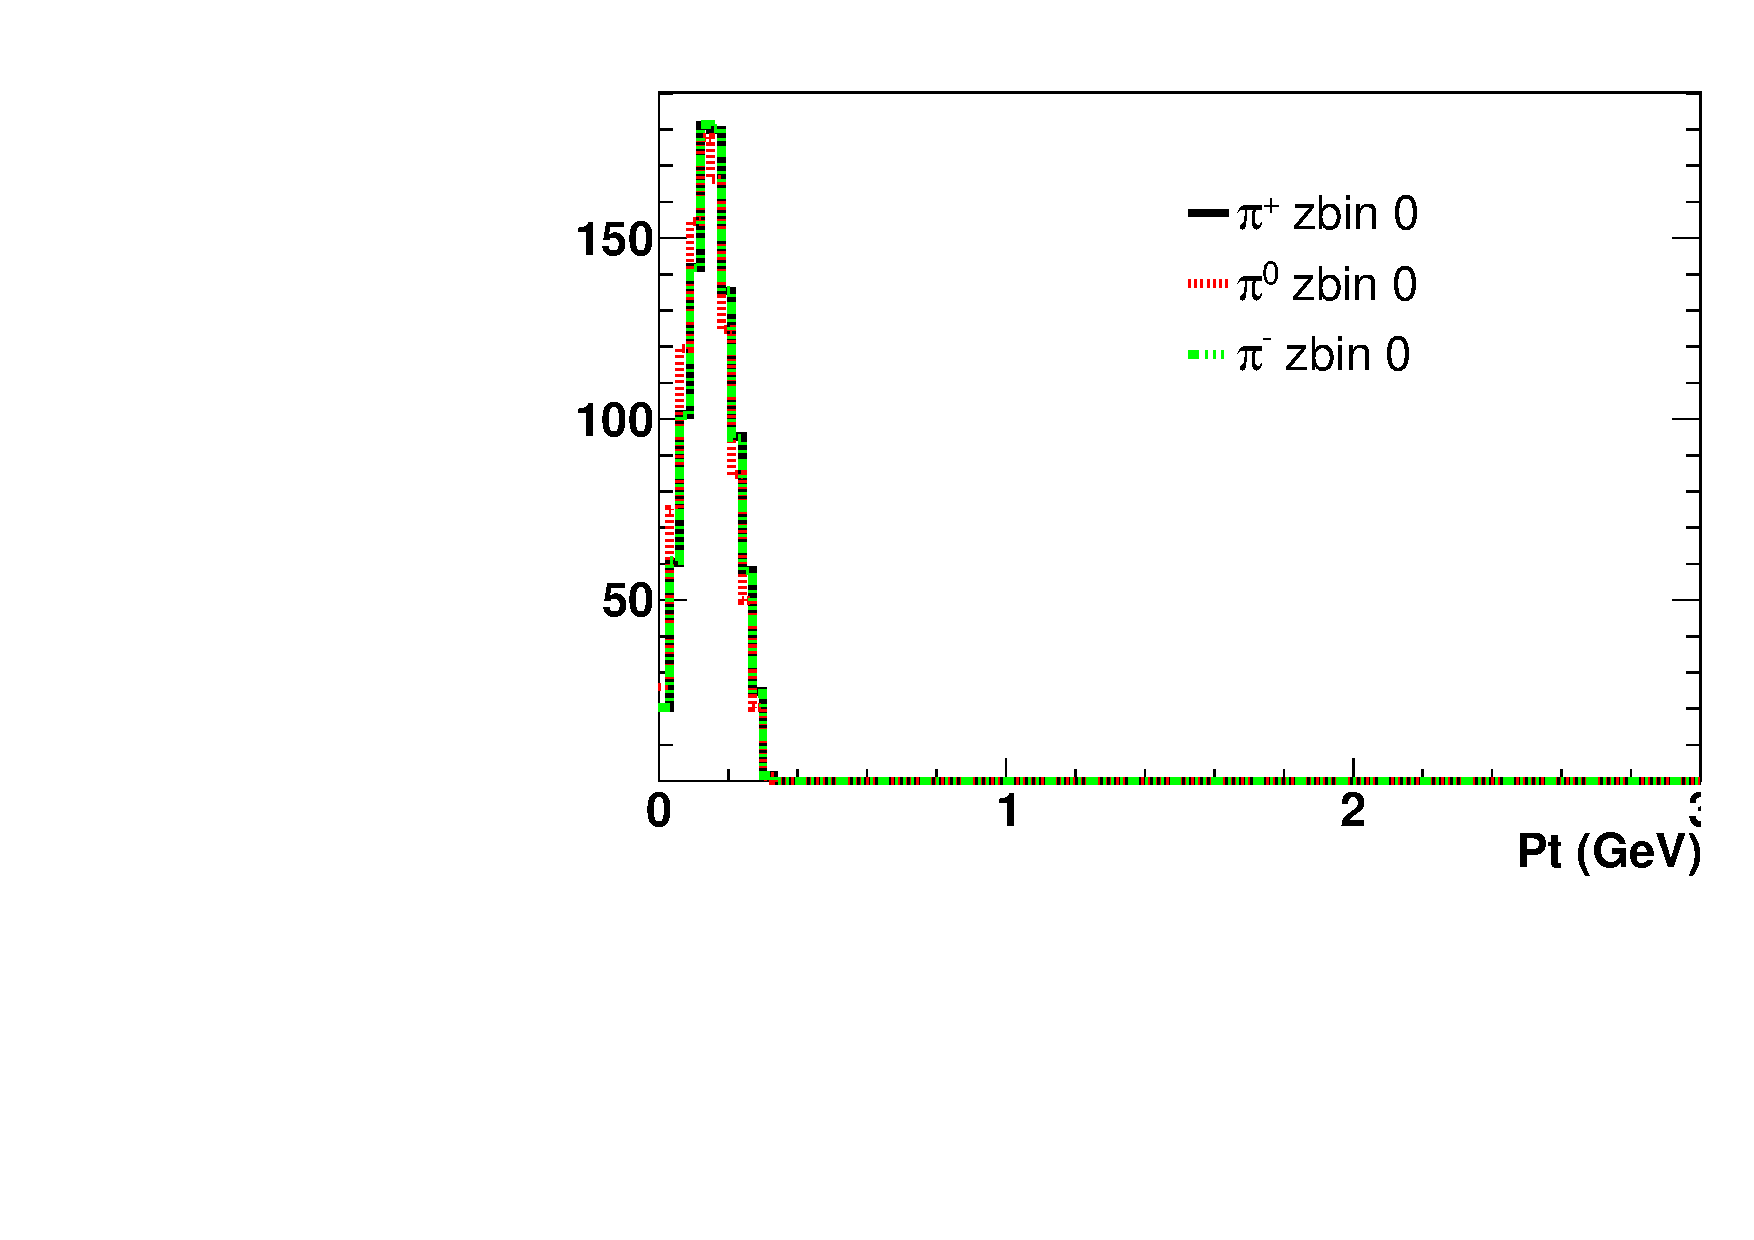
\includegraphics[width=.27\textwidth,natwidth=250,natheight=100]{figure_fiducial/had0.3/Pt_distri_for_zbin_0_norm_had03.pdf}
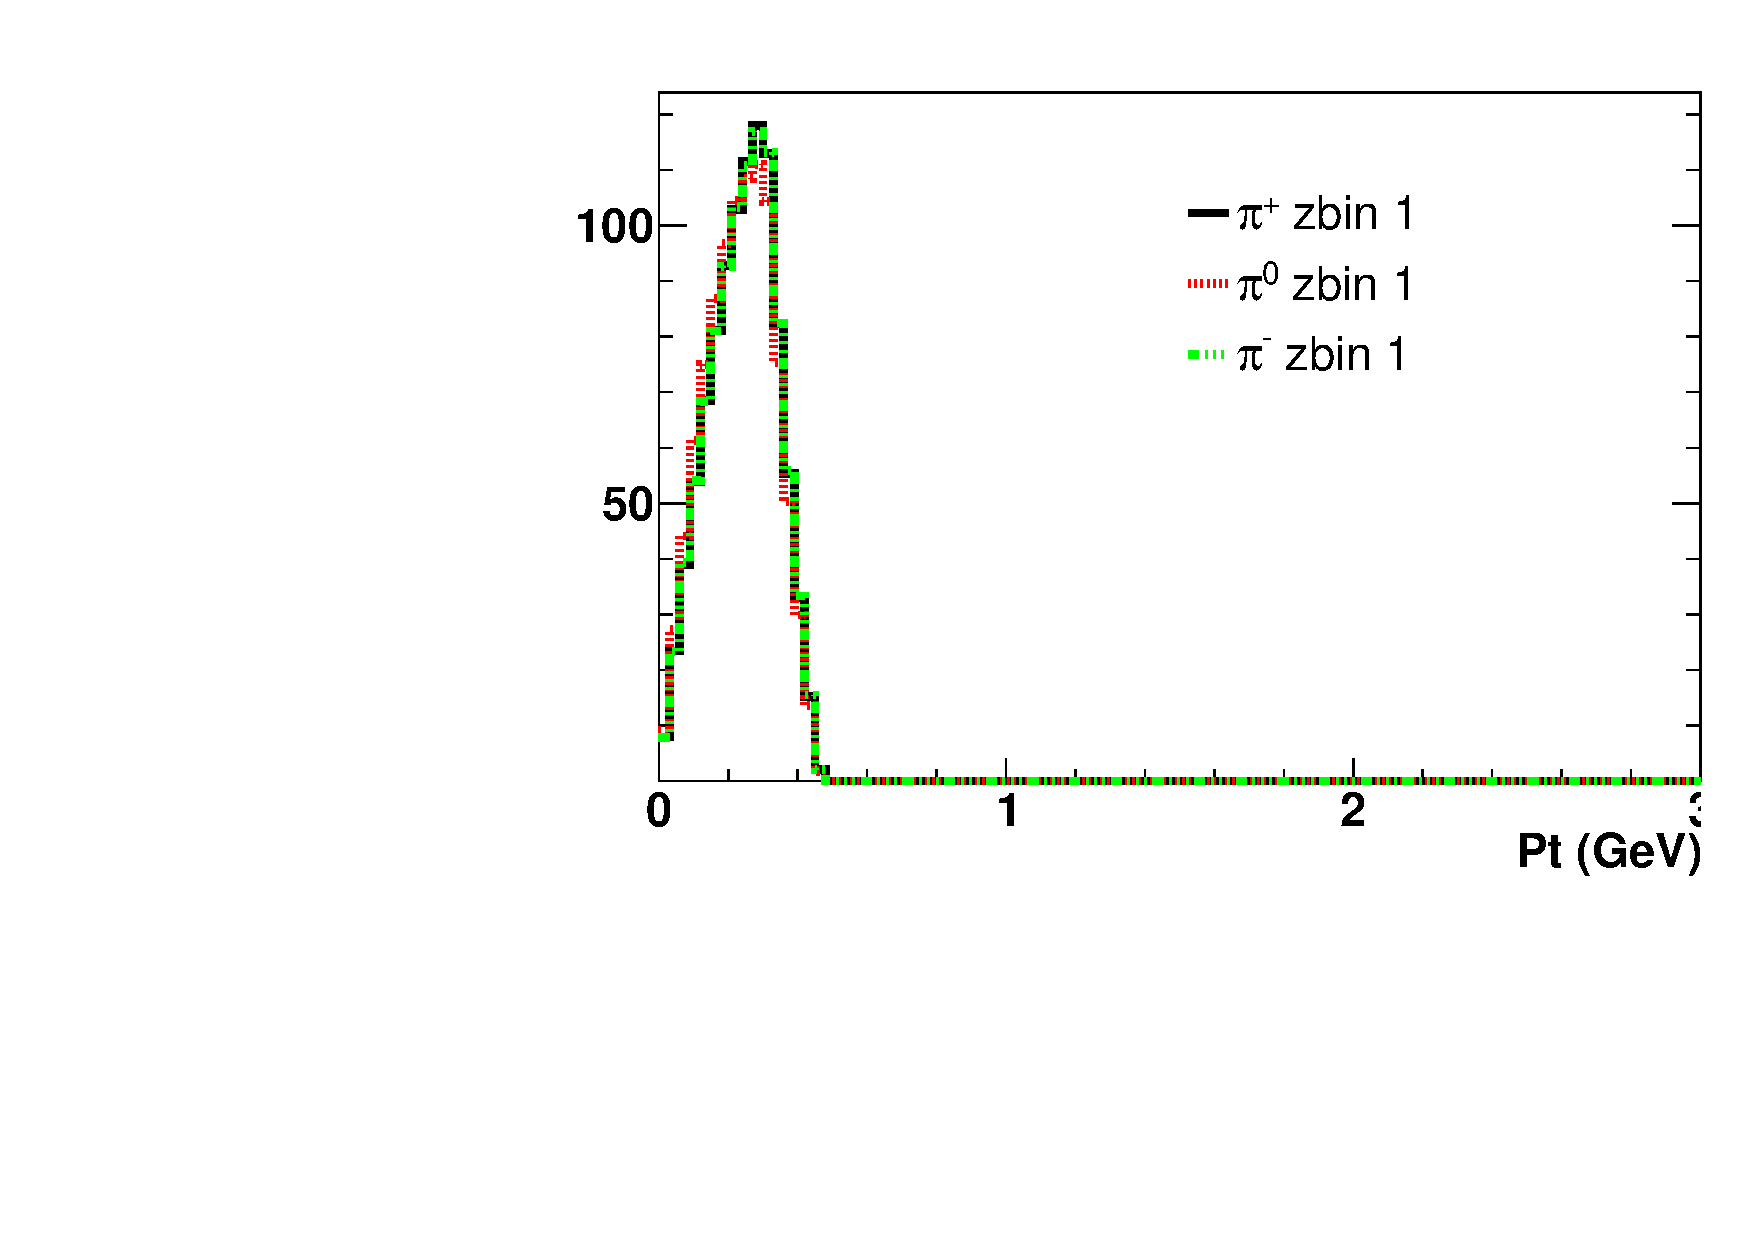
\includegraphics[width=.27\textwidth,natwidth=250,natheight=100]{figure_fiducial/had0.3/Pt_distri_for_zbin_1_norm_had03.pdf}
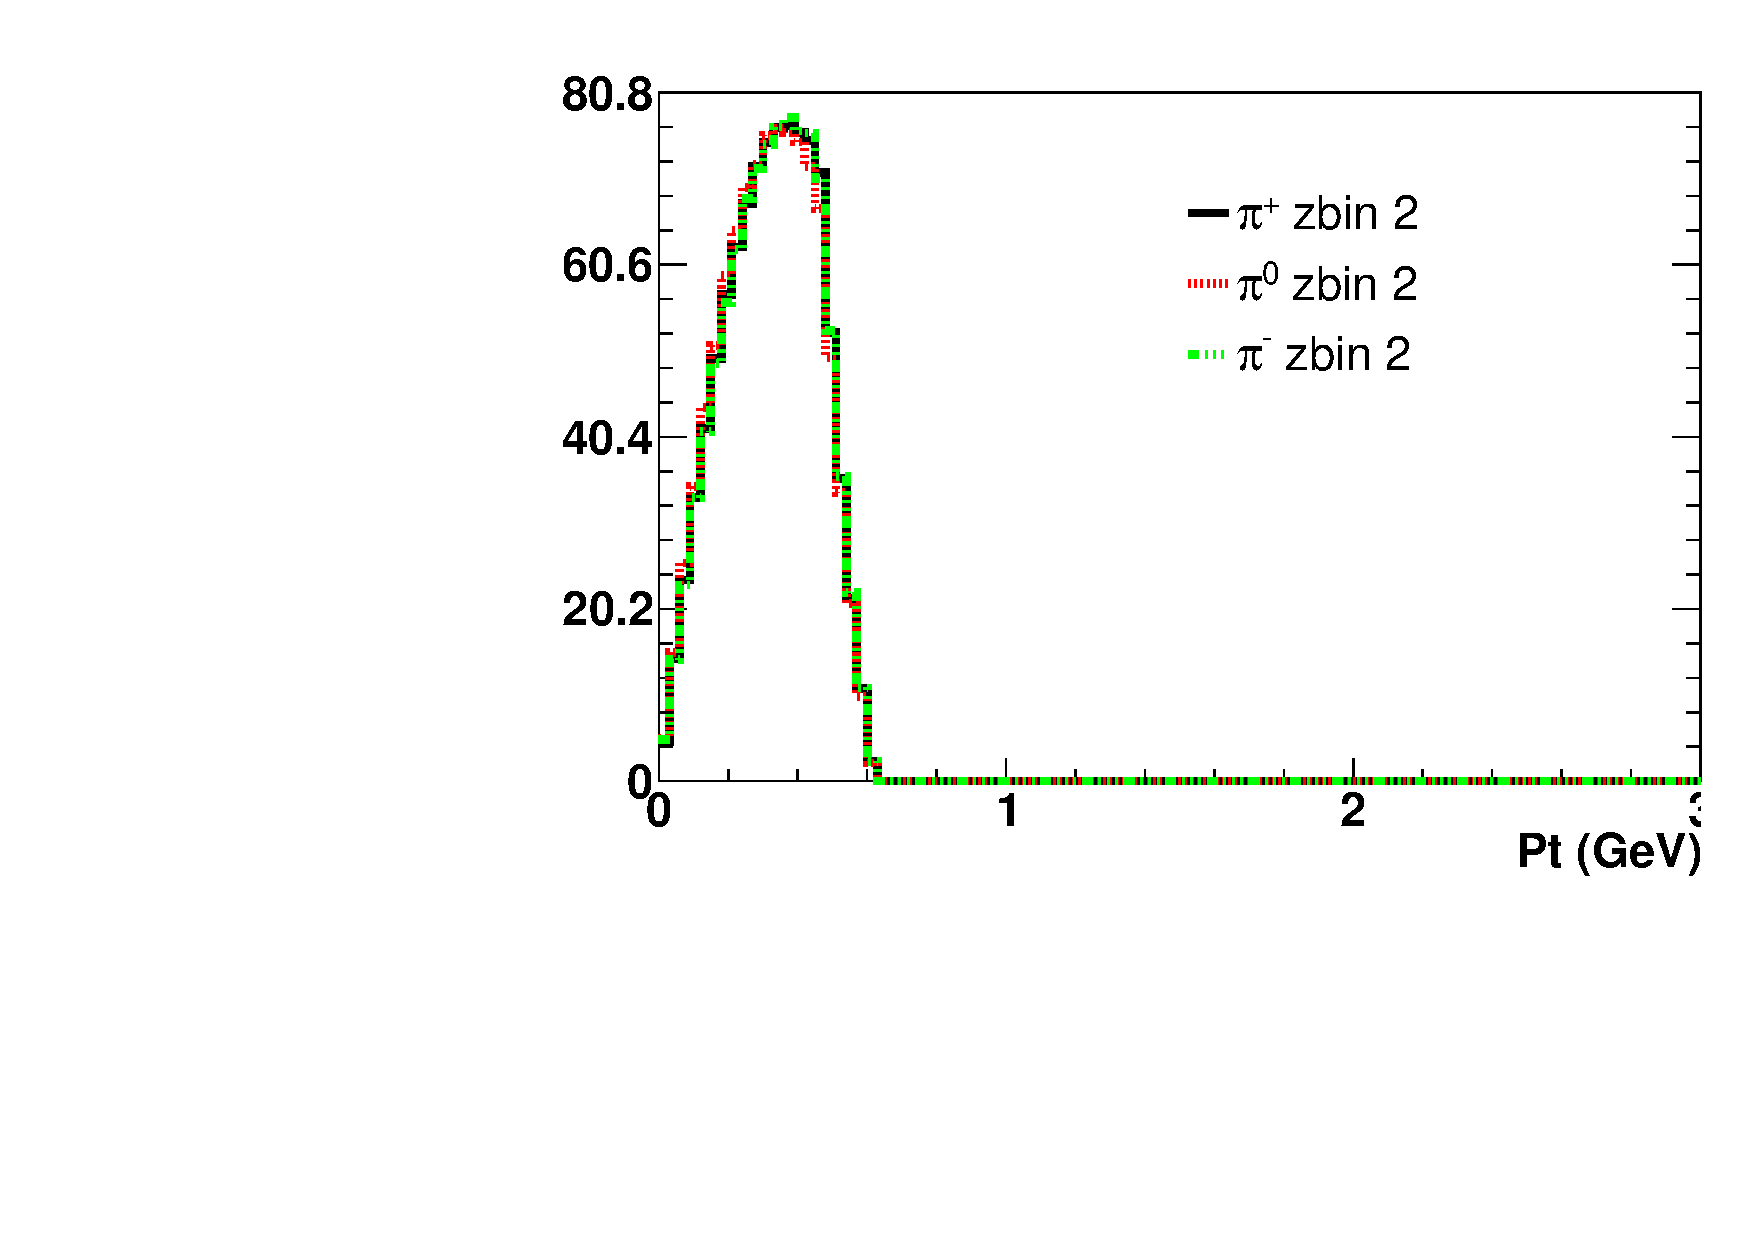
\includegraphics[width=.27\textwidth,natwidth=250,natheight=100]{figure_fiducial/had0.3/Pt_distri_for_zbin_2_norm_had03.pdf}\hfill
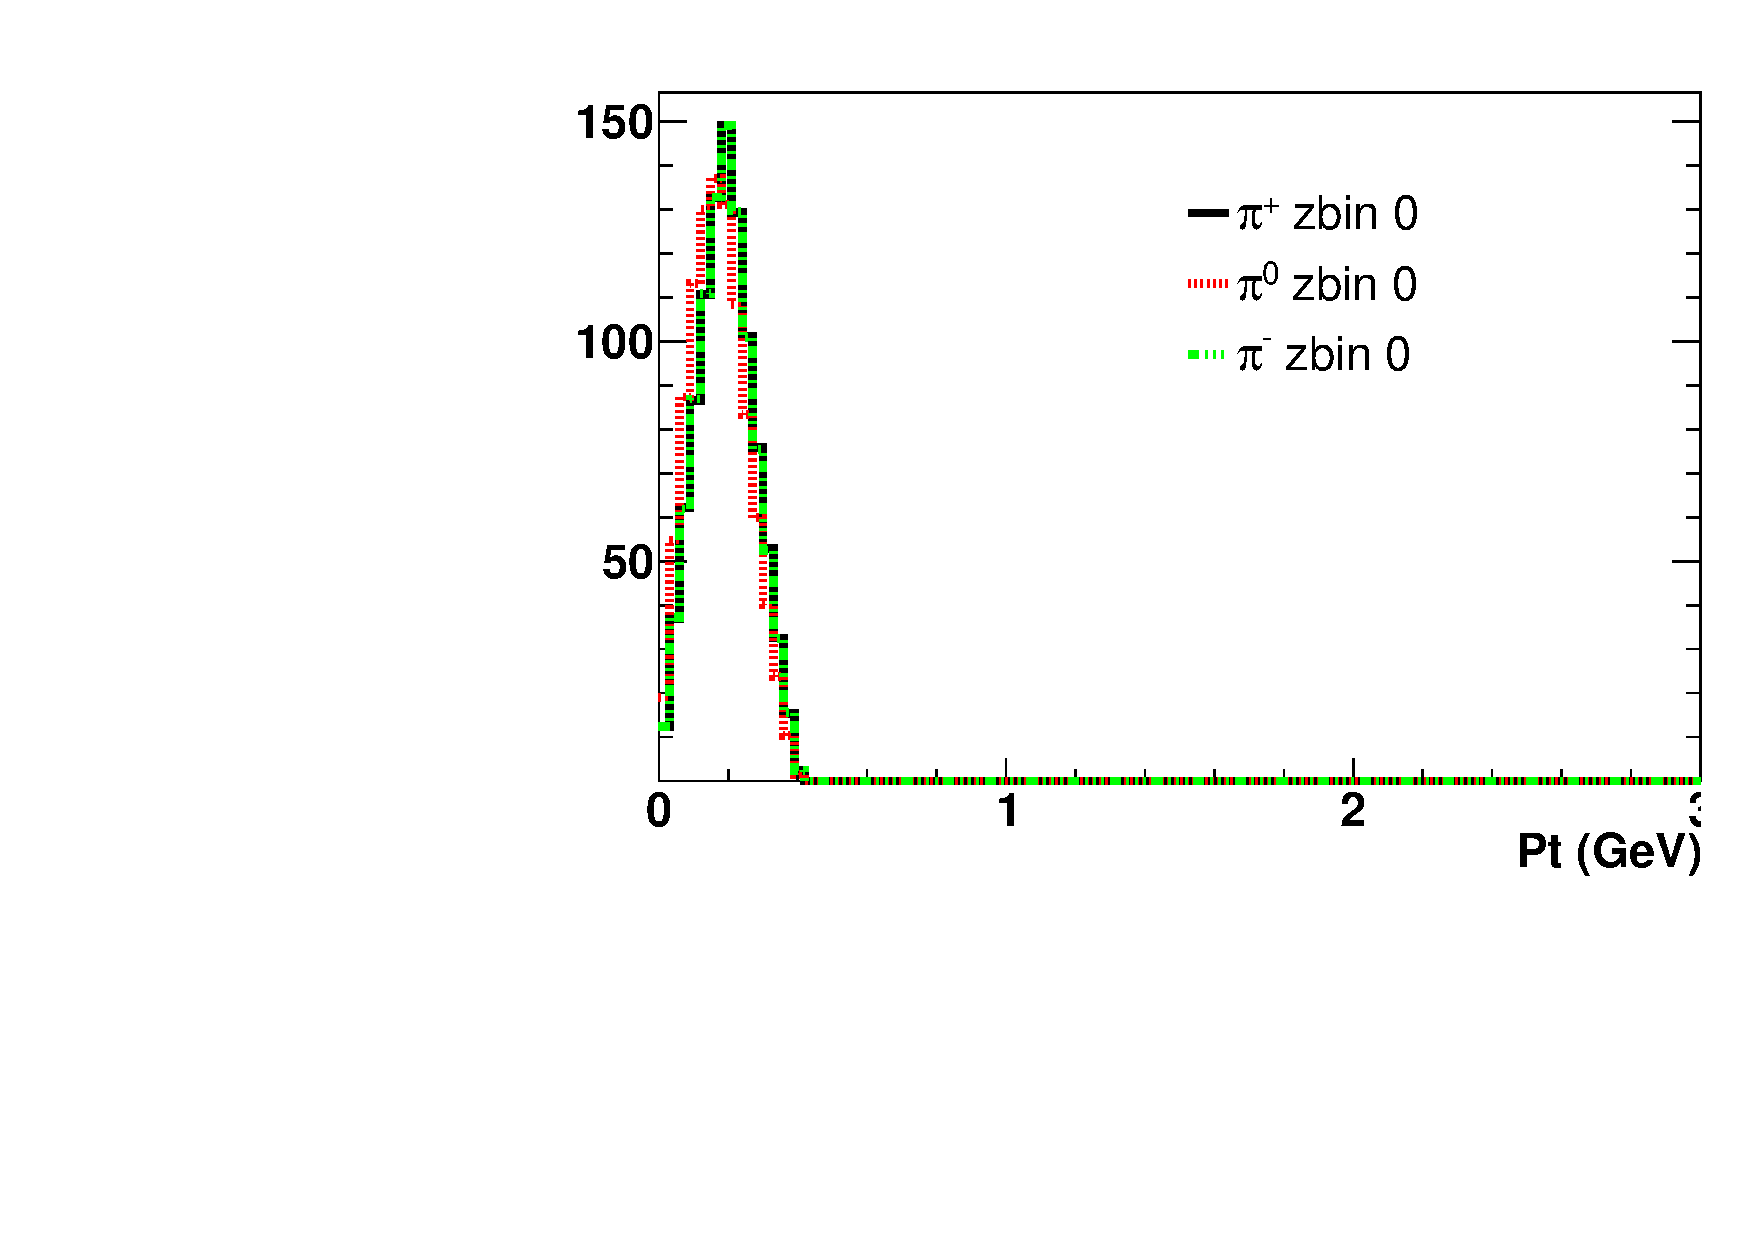
\includegraphics[width=.27\textwidth,natwidth=250,natheight=100]{figure_fiducial/had0.4/Pt_distri_for_zbin_0_norm_had04.pdf}
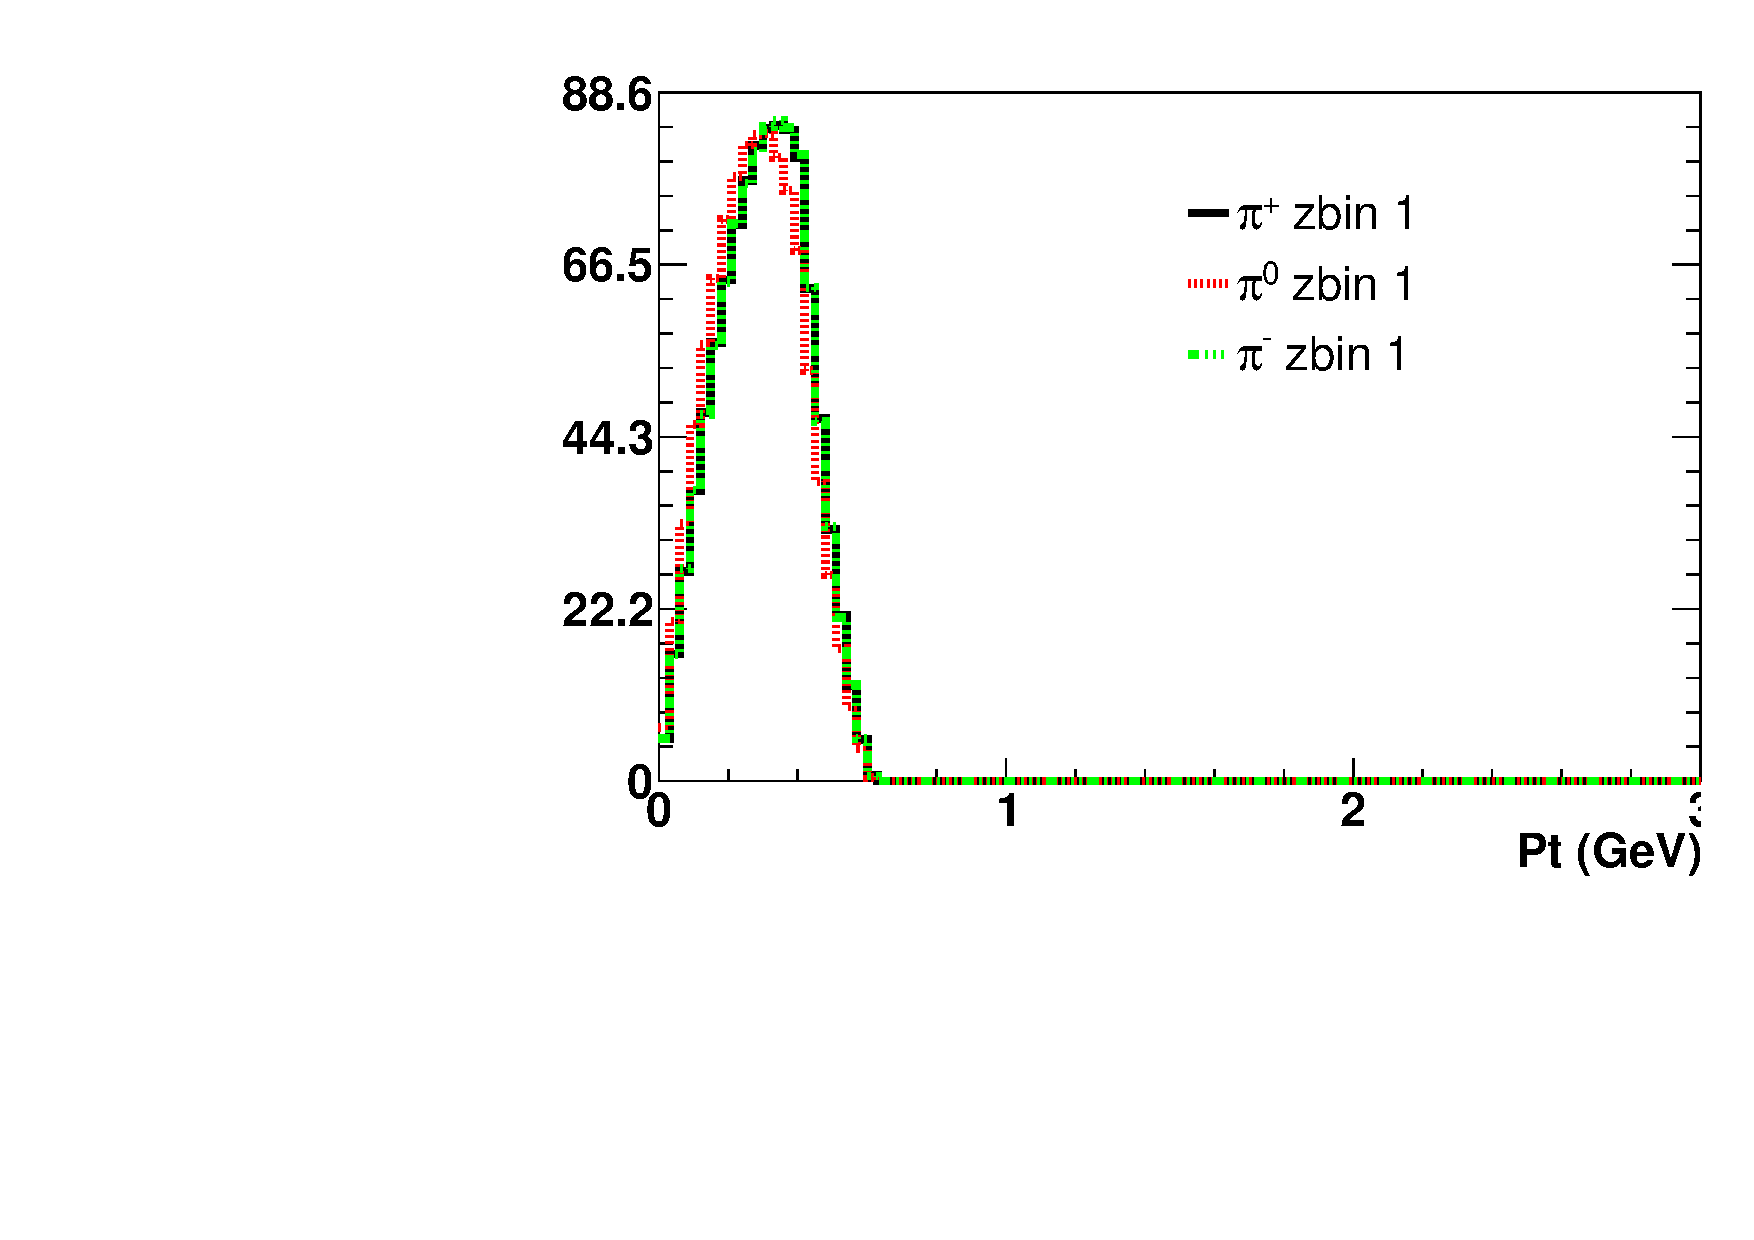
\includegraphics[width=.27\textwidth,natwidth=250,natheight=100]{figure_fiducial/had0.4/Pt_distri_for_zbin_1_norm_had04.pdf}
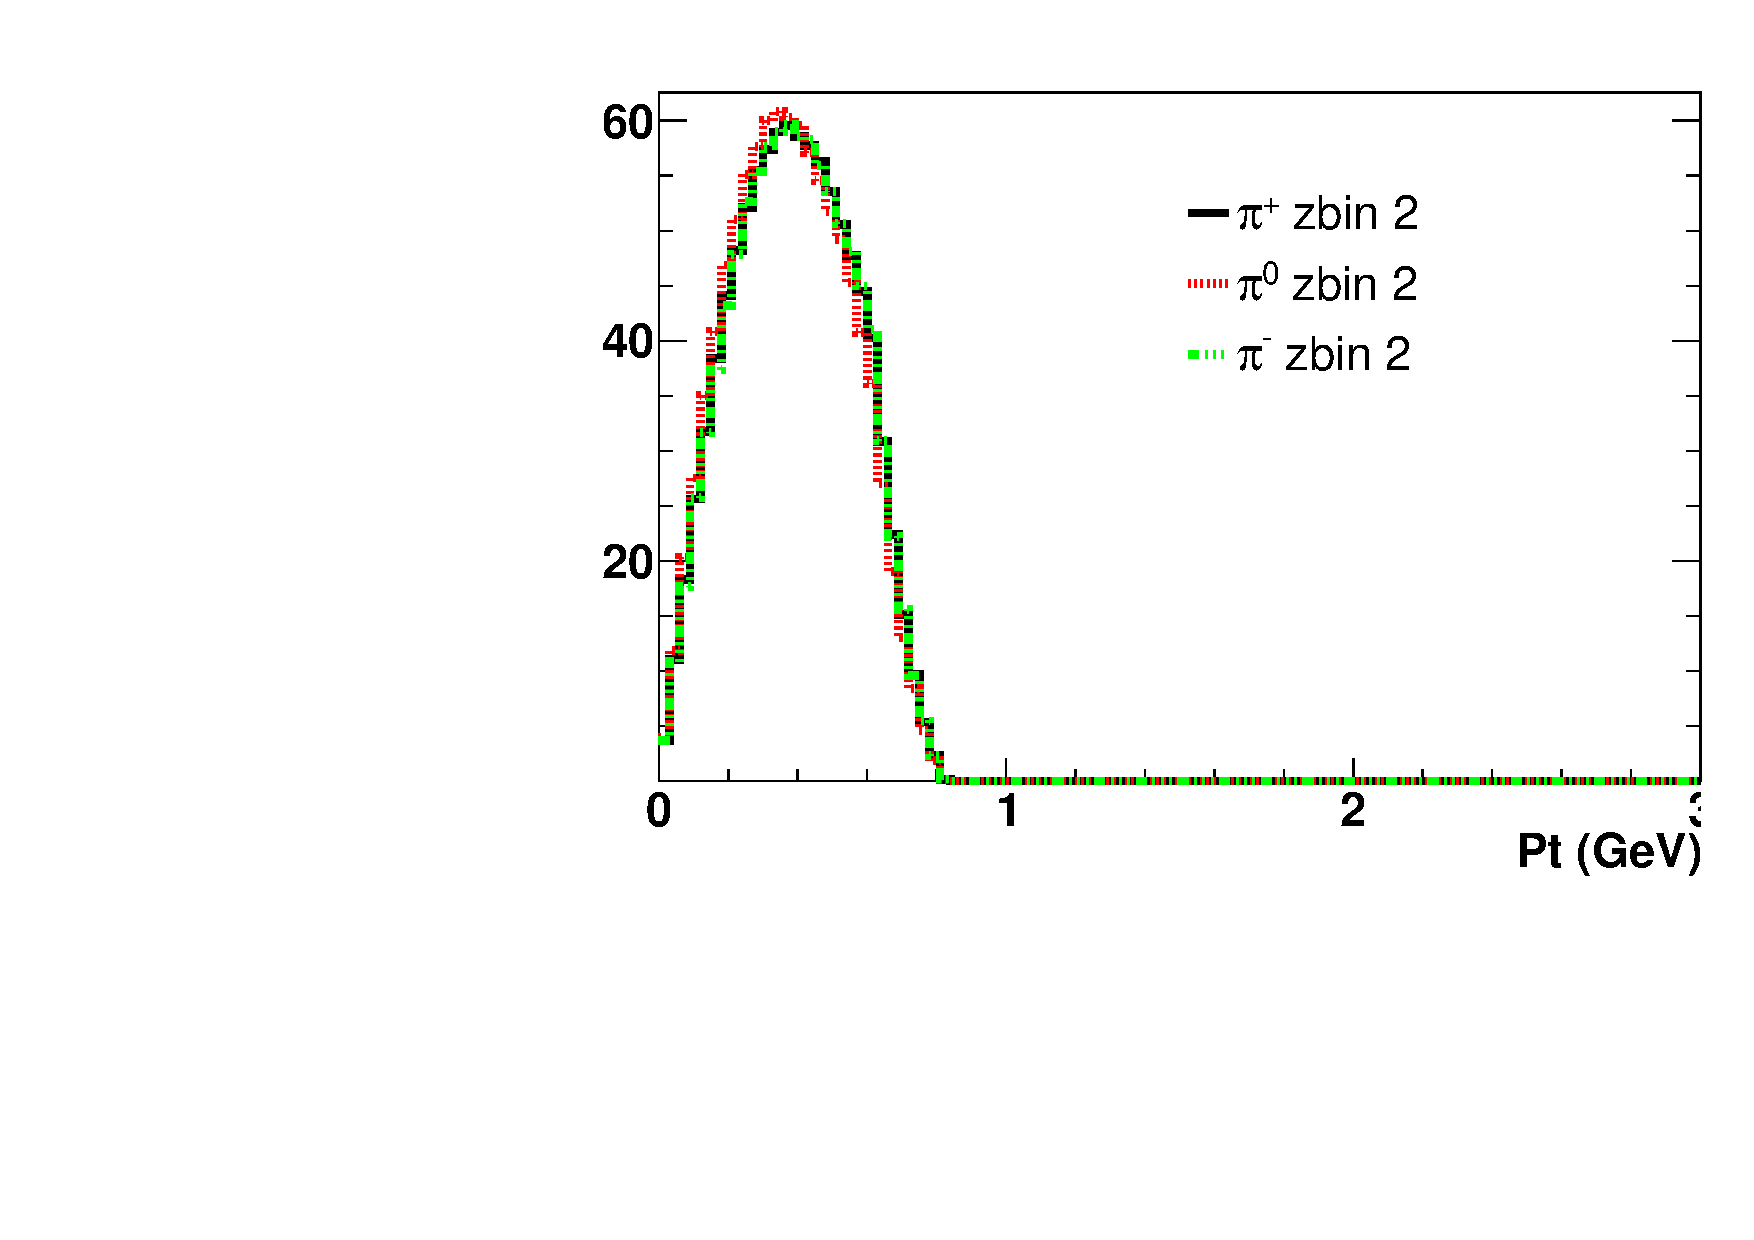
\includegraphics[width=.27\textwidth,natwidth=250,natheight=100]{figure_fiducial/had0.4/Pt_distri_for_zbin_2_norm_had04.pdf}\hfill
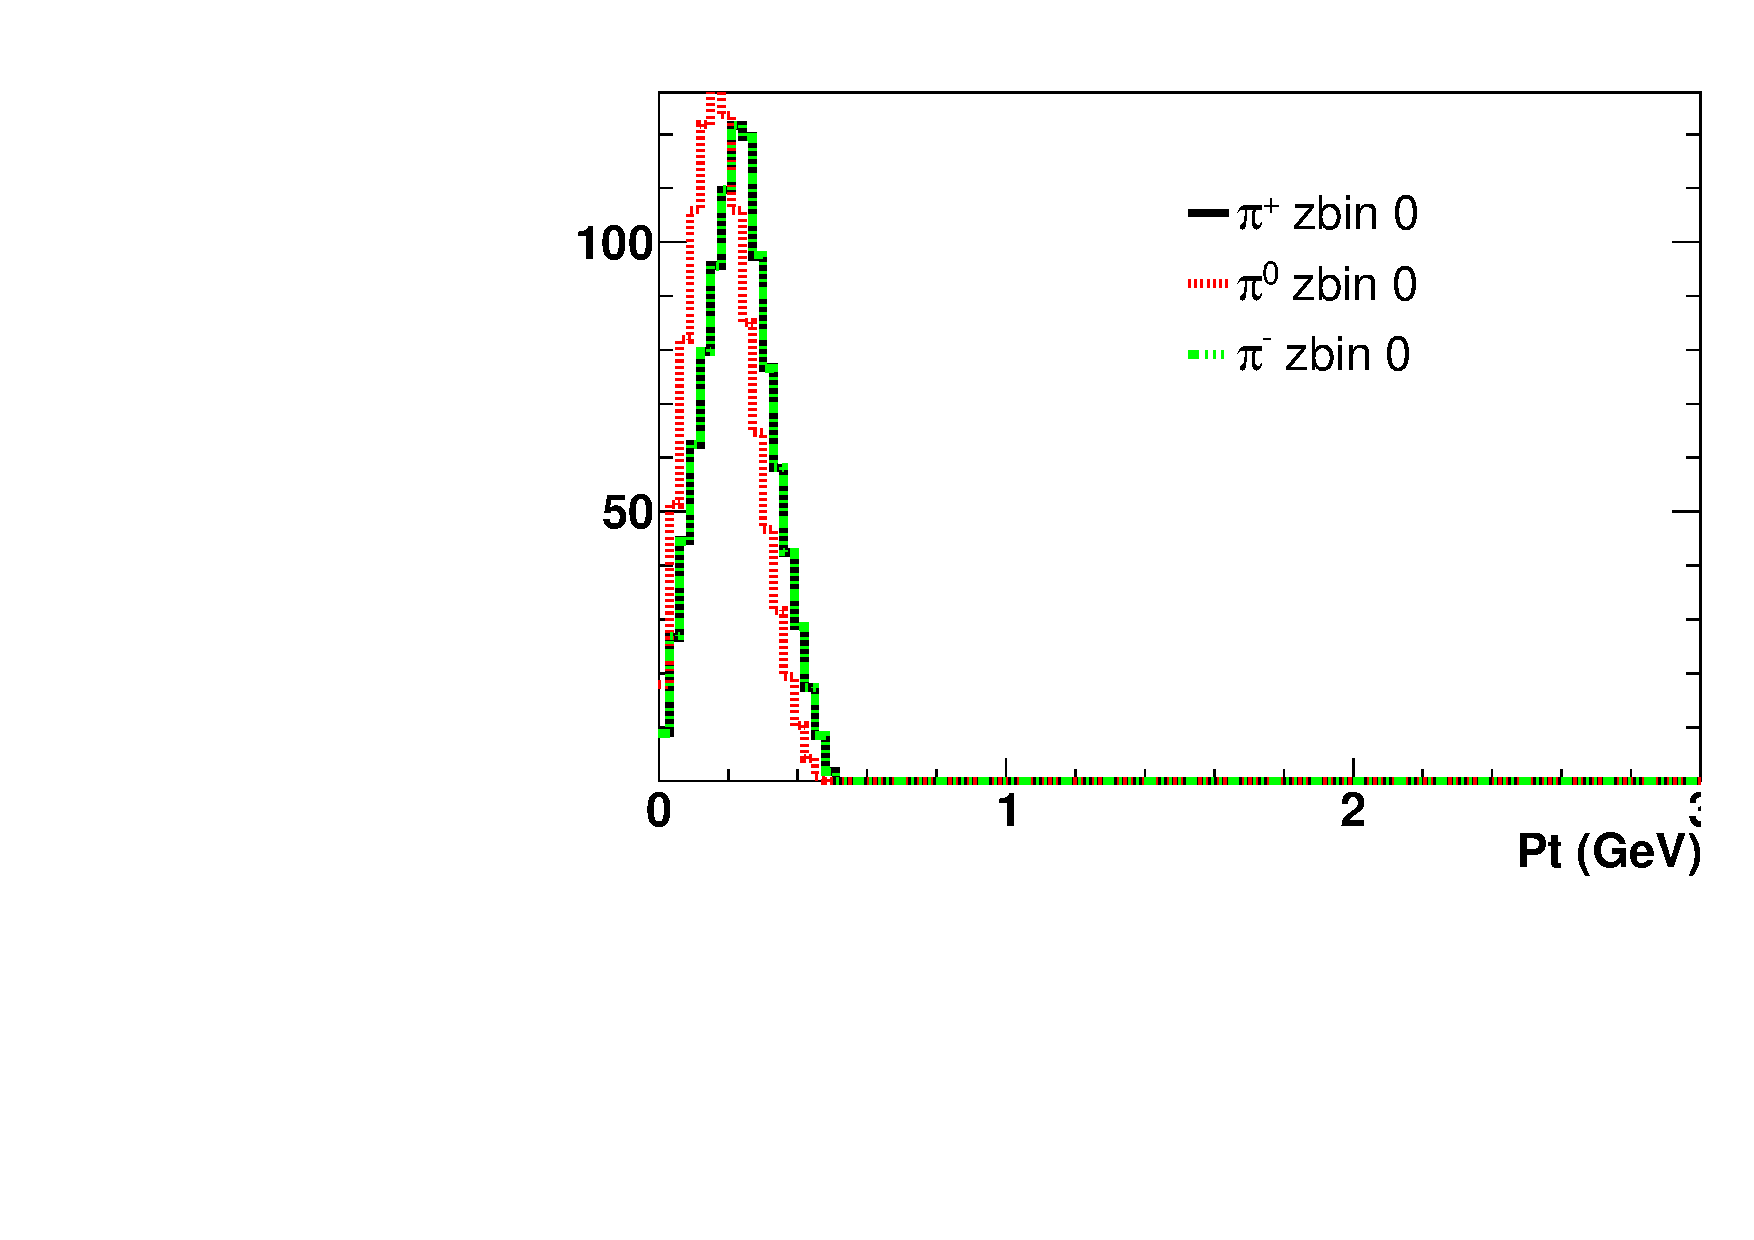
\includegraphics[width=.27\textwidth,natwidth=250,natheight=100]{figure_fiducial/had0.5/Pt_distri_for_zbin_0_norm_had05.pdf}
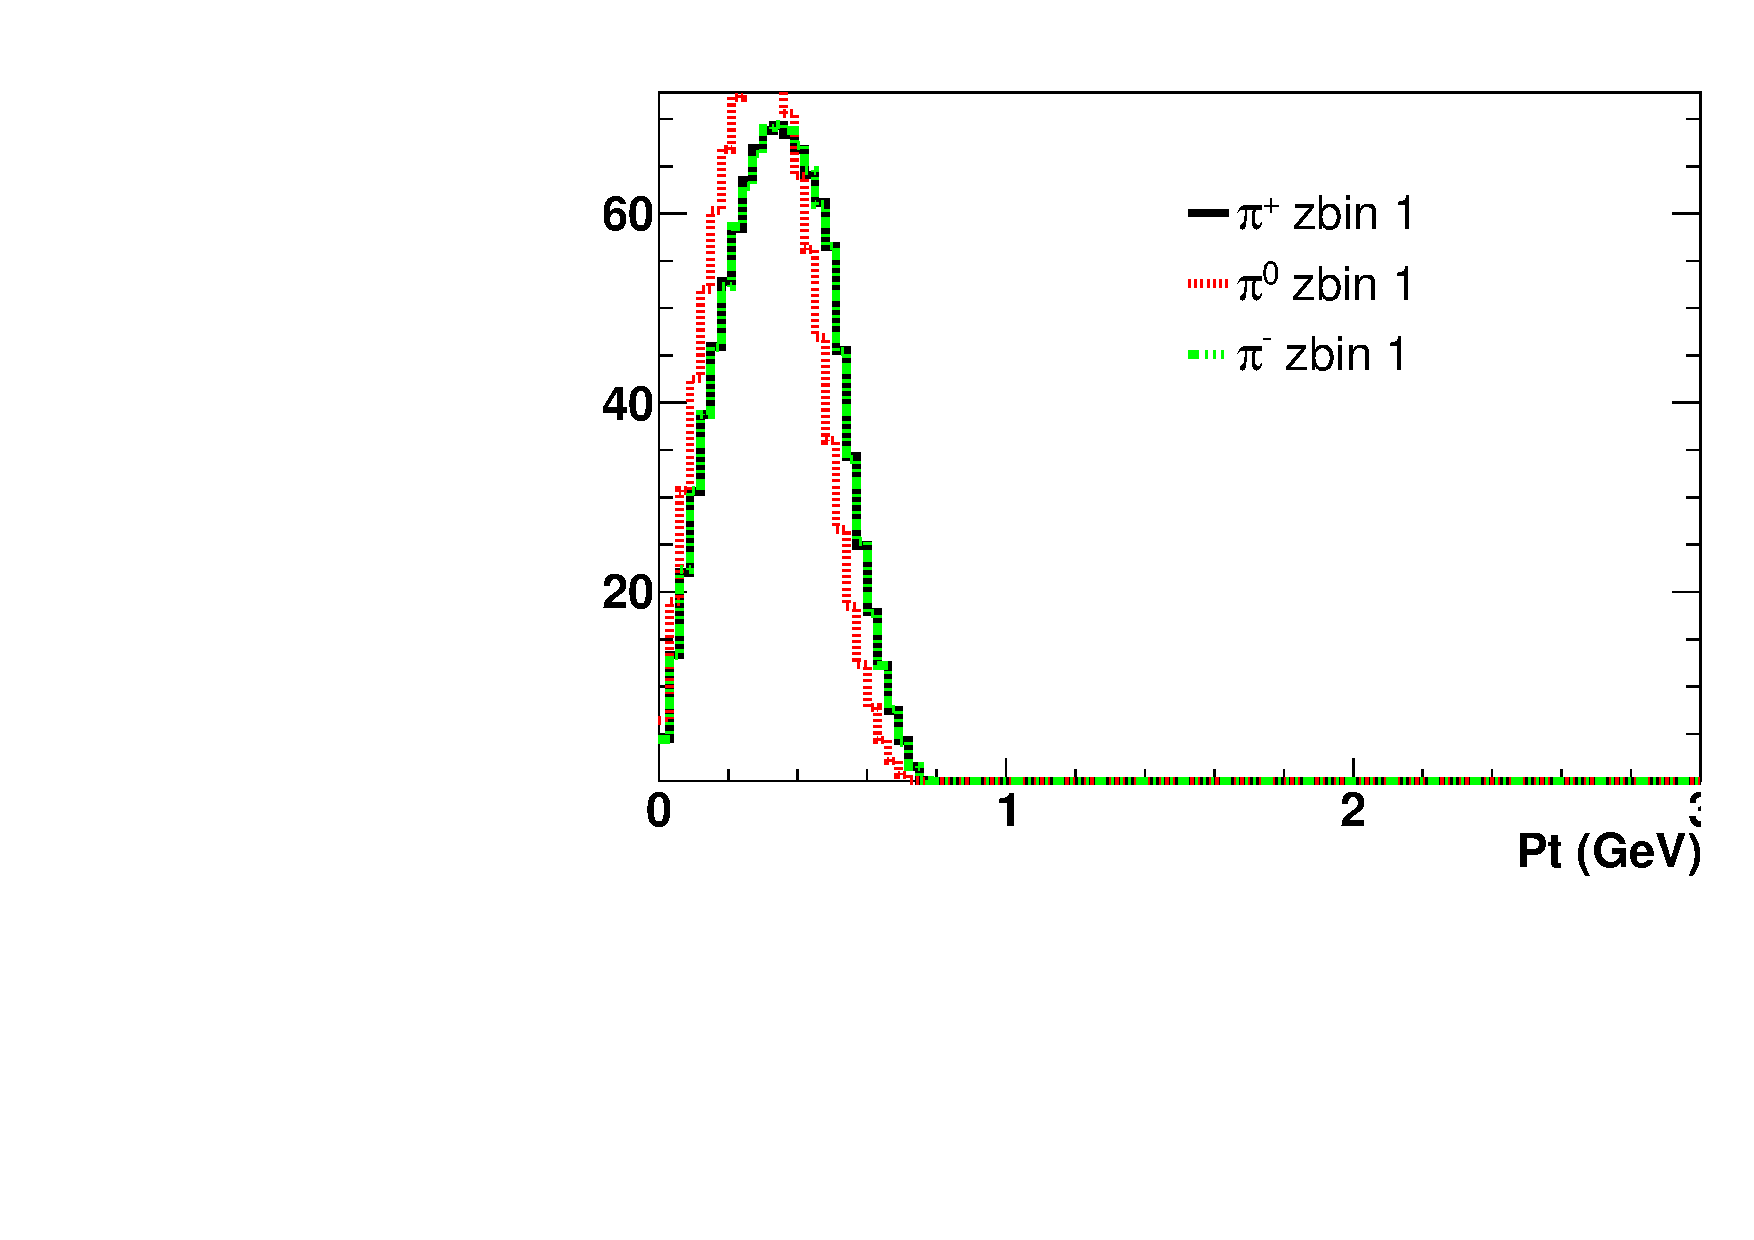
\includegraphics[width=.27\textwidth,natwidth=250,natheight=100]{figure_fiducial/had0.5/Pt_distri_for_zbin_1_norm_had05.pdf}
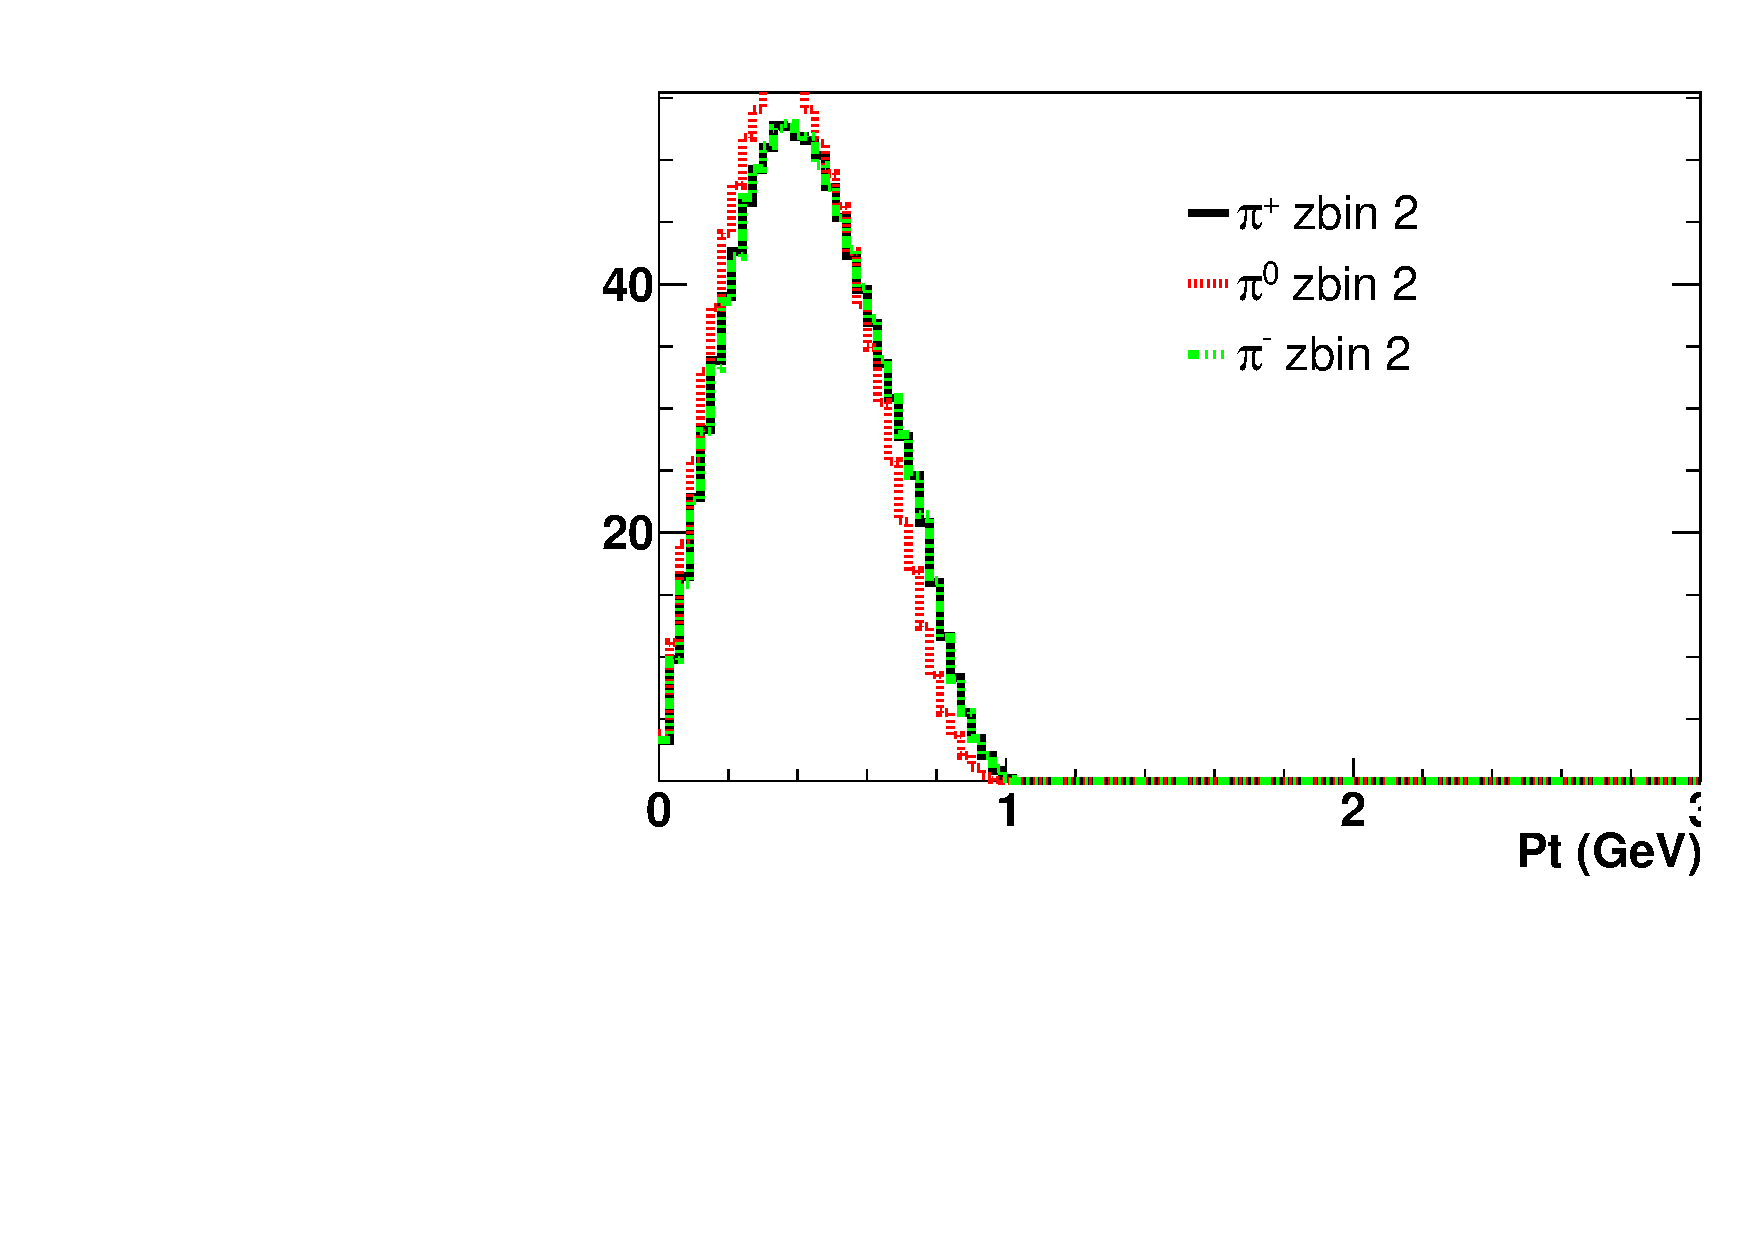
\includegraphics[width=.27\textwidth,natwidth=250,natheight=100]{figure_fiducial/had0.5/Pt_distri_for_zbin_2_norm_had05.pdf}\hfill
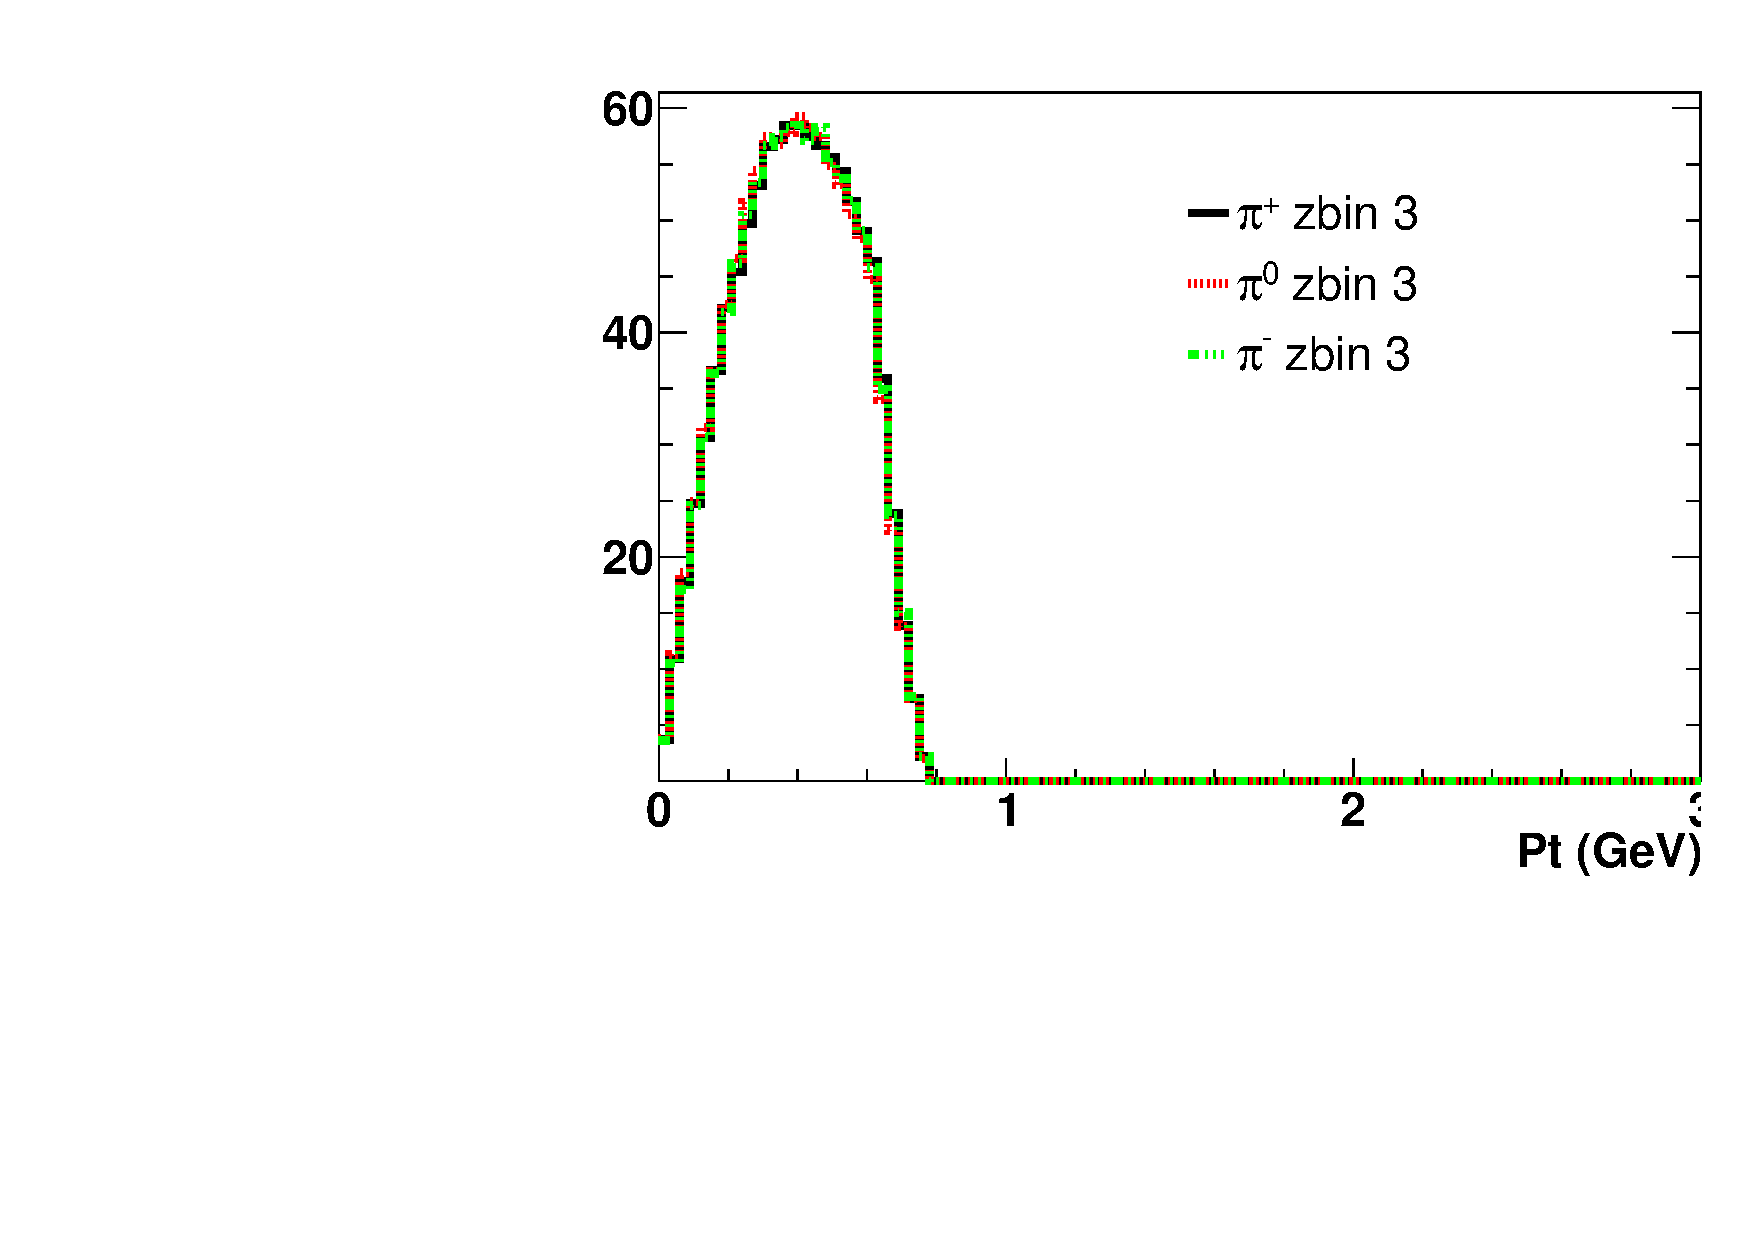
\includegraphics[width=.27\textwidth,natwidth=250,natheight=100]{figure_fiducial/had0.3/Pt_distri_for_zbin_3_norm_had03.pdf}
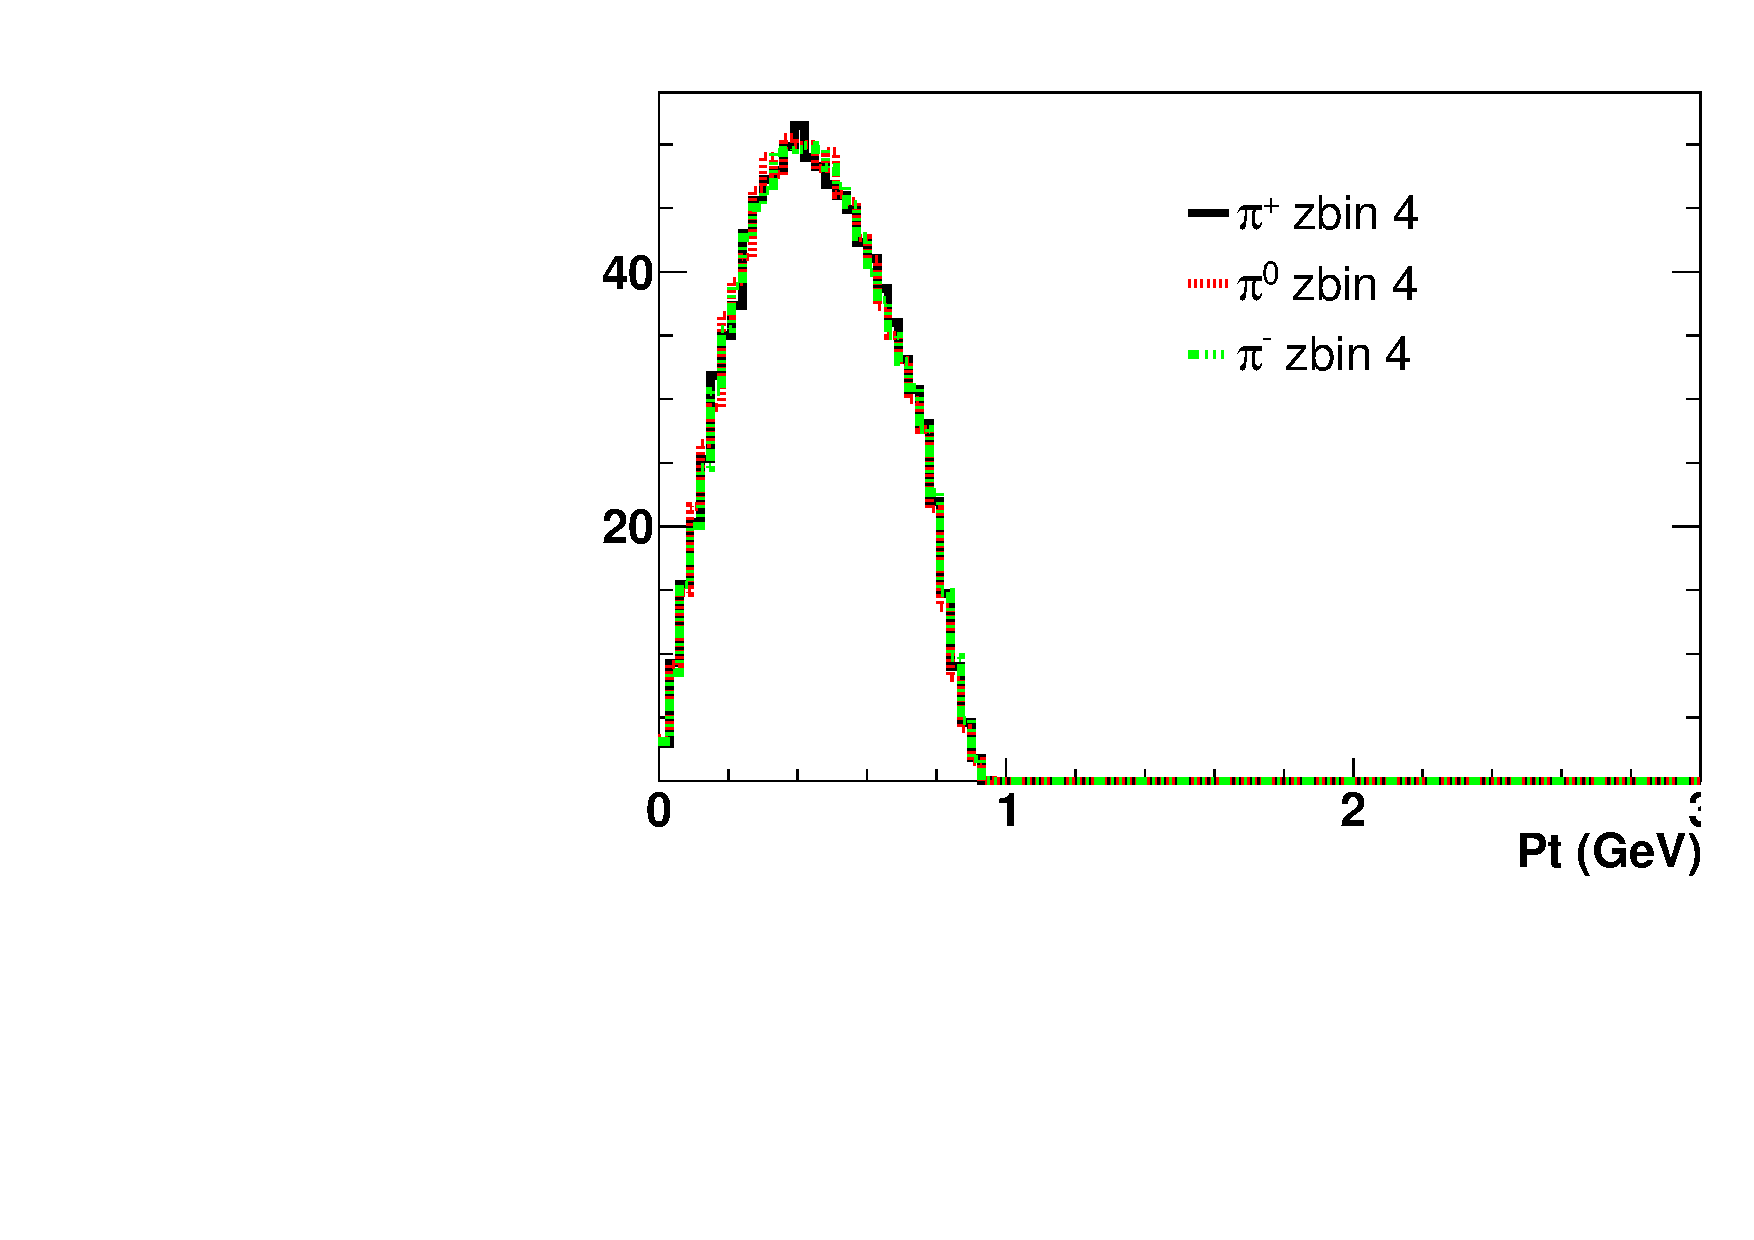
\includegraphics[width=.27\textwidth,natwidth=250,natheight=100]{figure_fiducial/had0.3/Pt_distri_for_zbin_4_norm_had03.pdf}
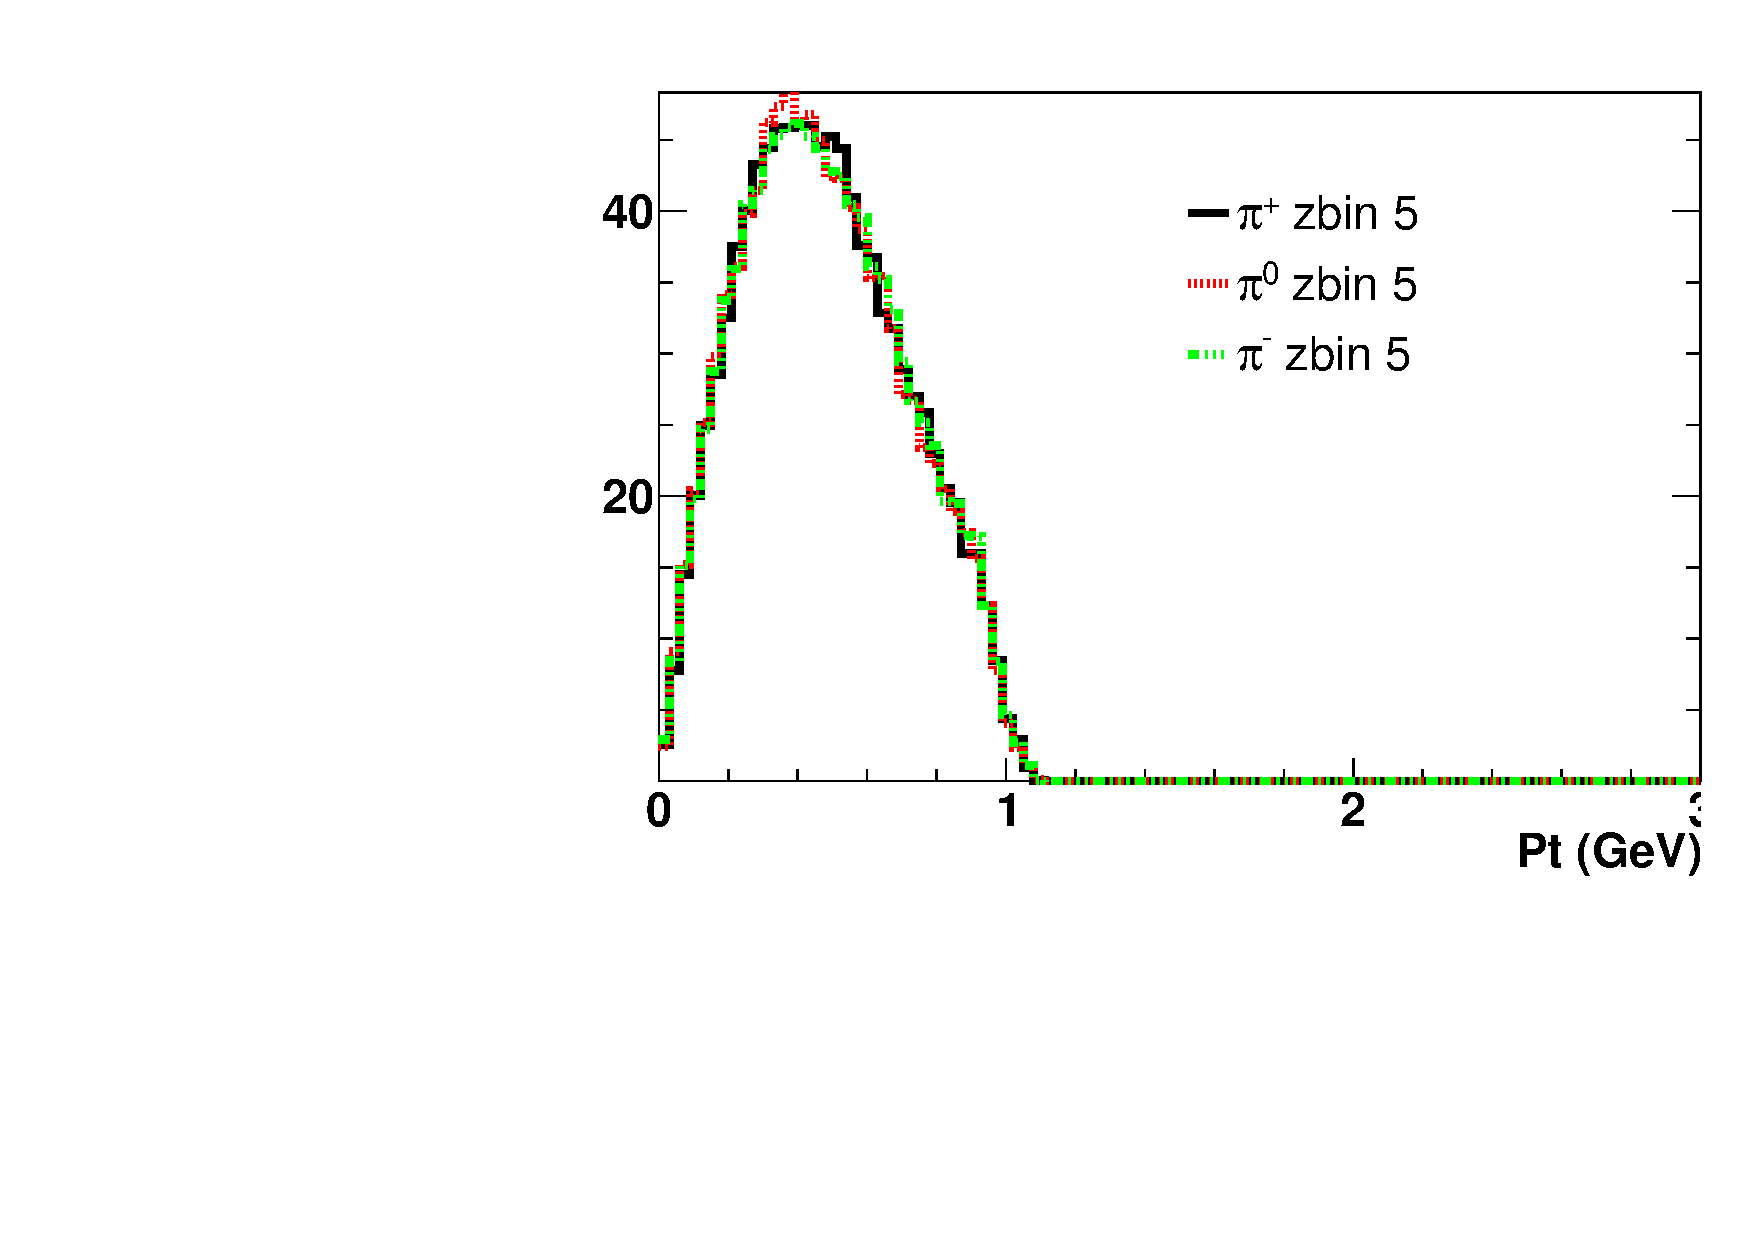
\includegraphics[width=.27\textwidth,natwidth=250,natheight=100]{figure_fiducial/had0.3/Pt_distri_for_zbin_5_norm_had03.pdf}\hfill
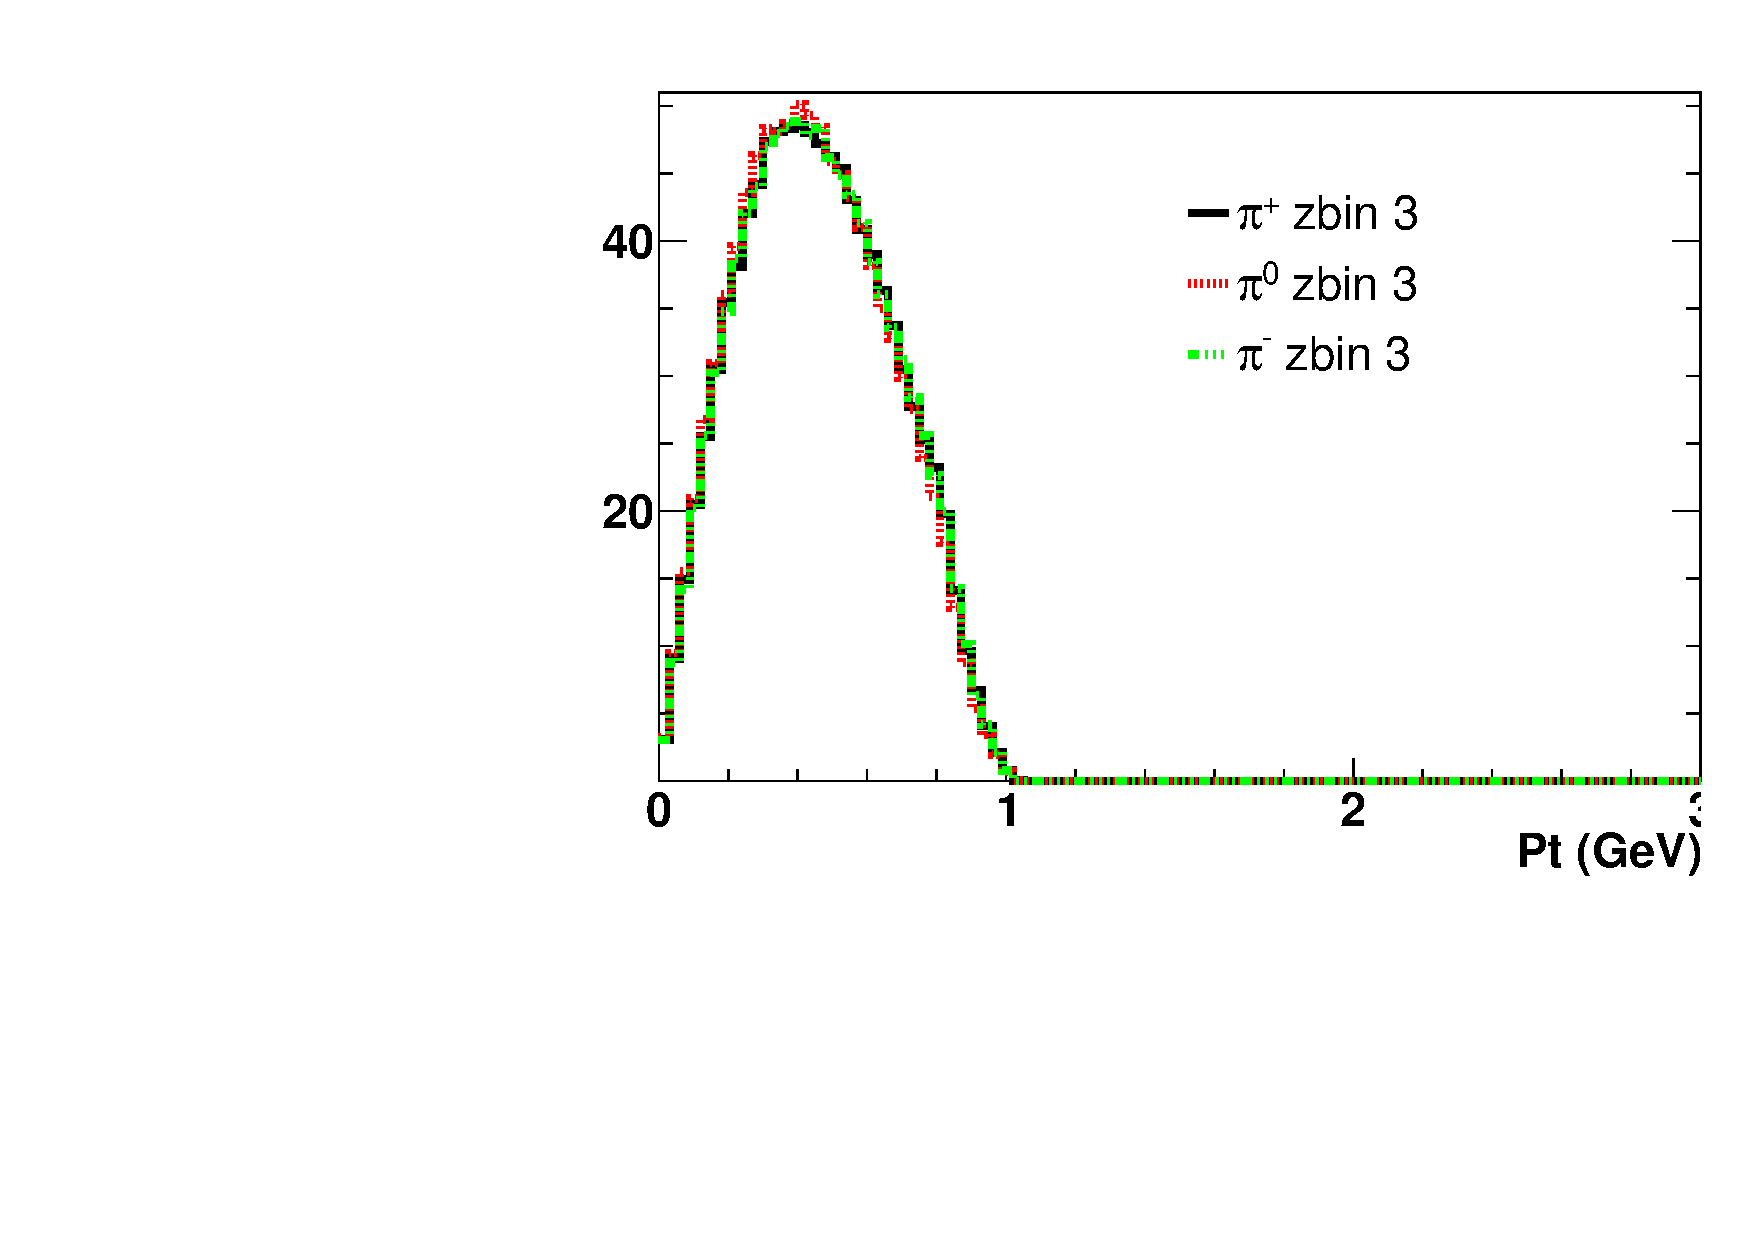
\includegraphics[width=.27\textwidth,natwidth=250,natheight=100]{figure_fiducial/had0.4/Pt_distri_for_zbin_3_norm_had04.pdf}
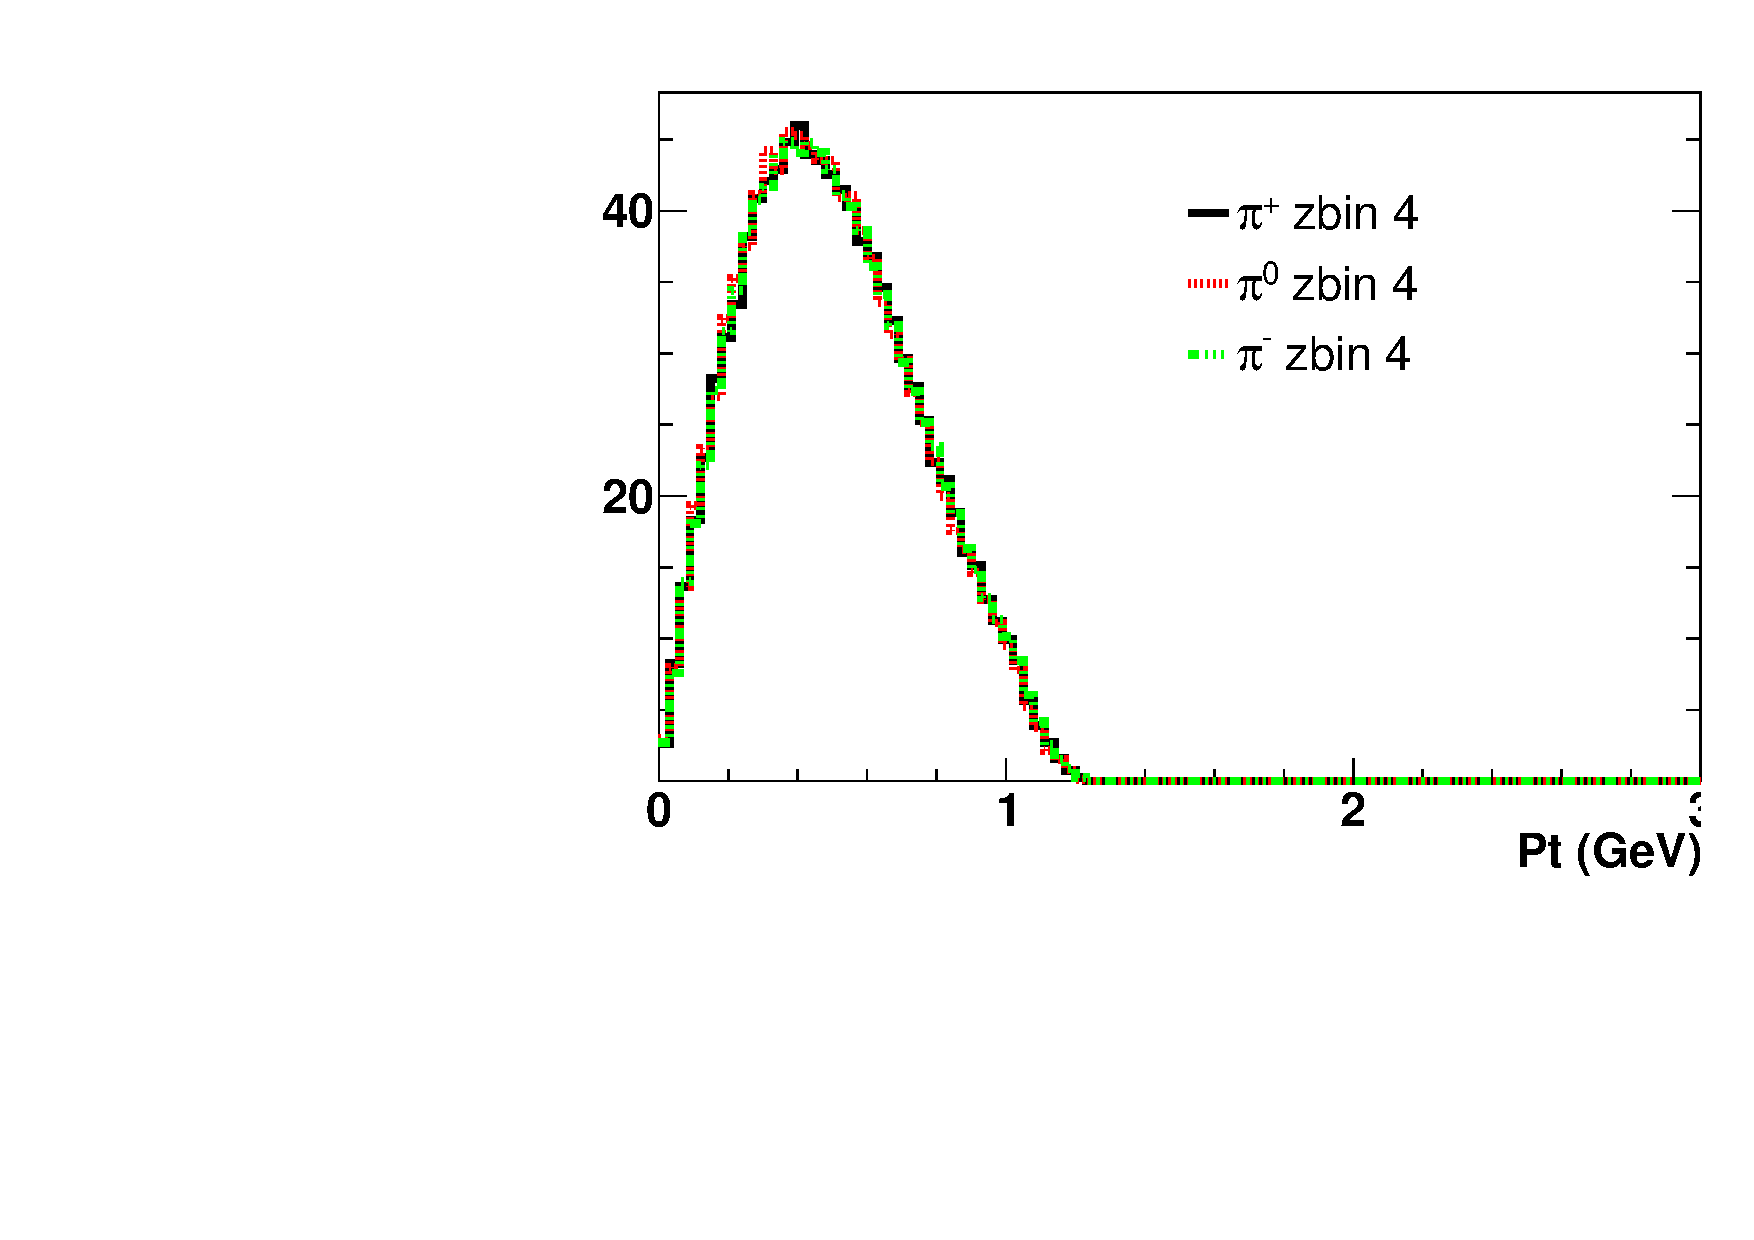
\includegraphics[width=.27\textwidth,natwidth=250,natheight=100]{figure_fiducial/had0.4/Pt_distri_for_zbin_4_norm_had04.pdf}
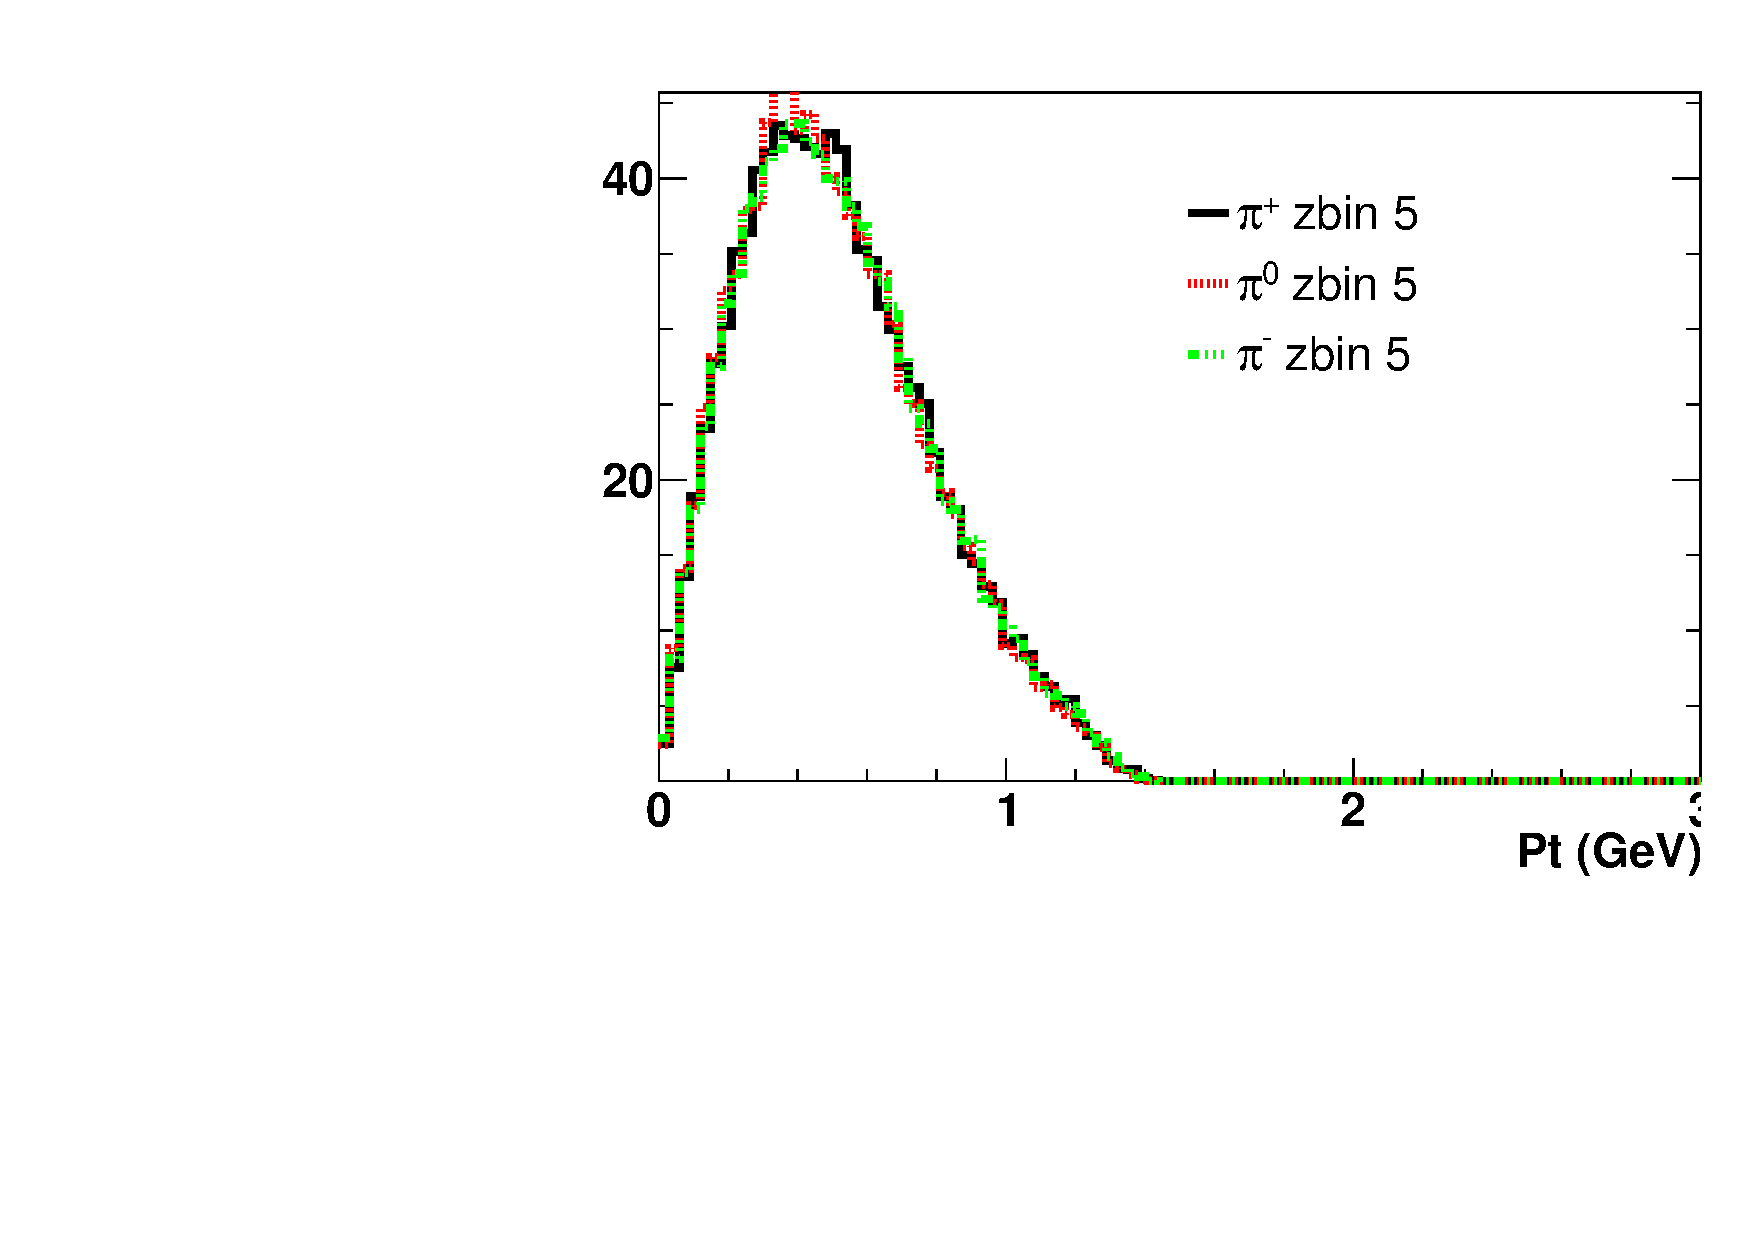
\includegraphics[width=.27\textwidth,natwidth=250,natheight=100]{figure_fiducial/had0.4/Pt_distri_for_zbin_5_norm_had04.pdf}\hfill
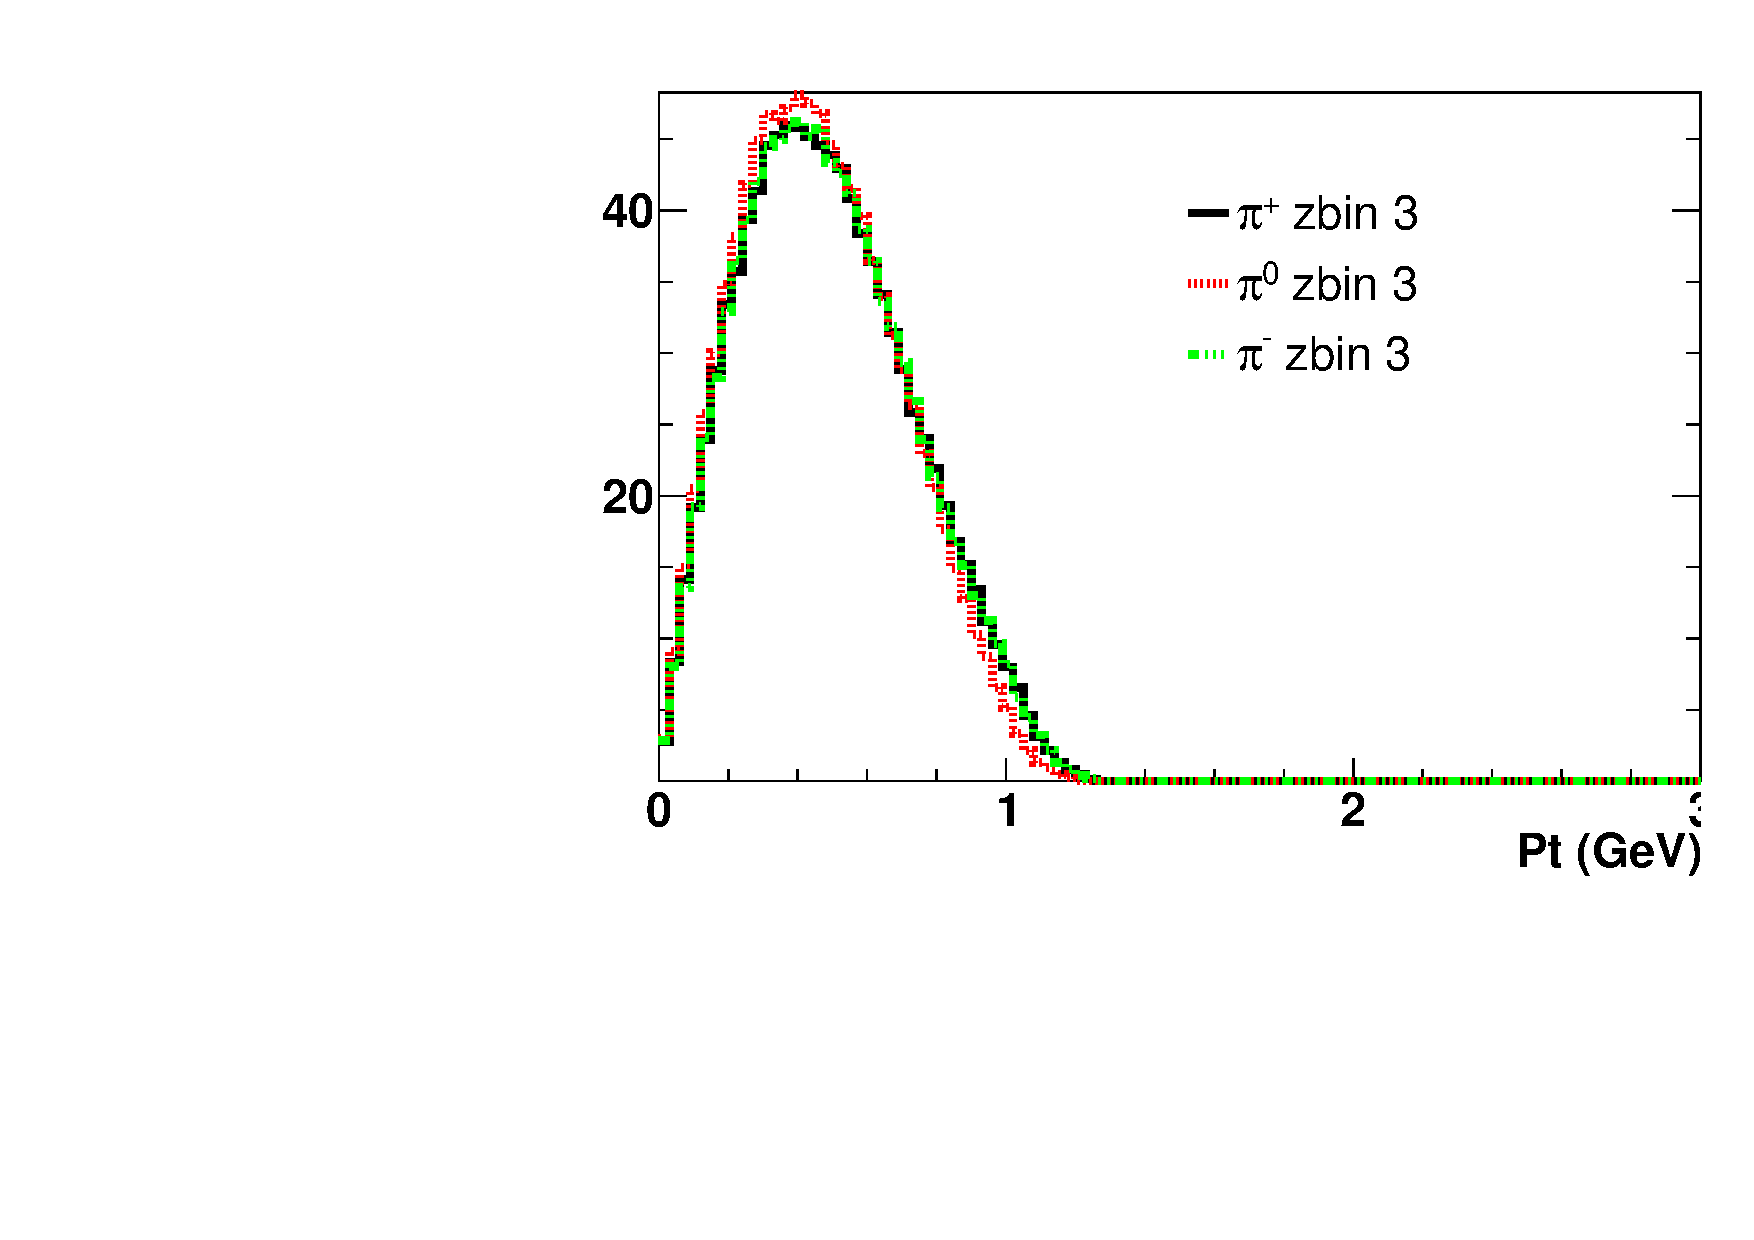
\includegraphics[width=.27\textwidth,natwidth=250,natheight=100]{figure_fiducial/had0.5/Pt_distri_for_zbin_3_norm_had05.pdf}
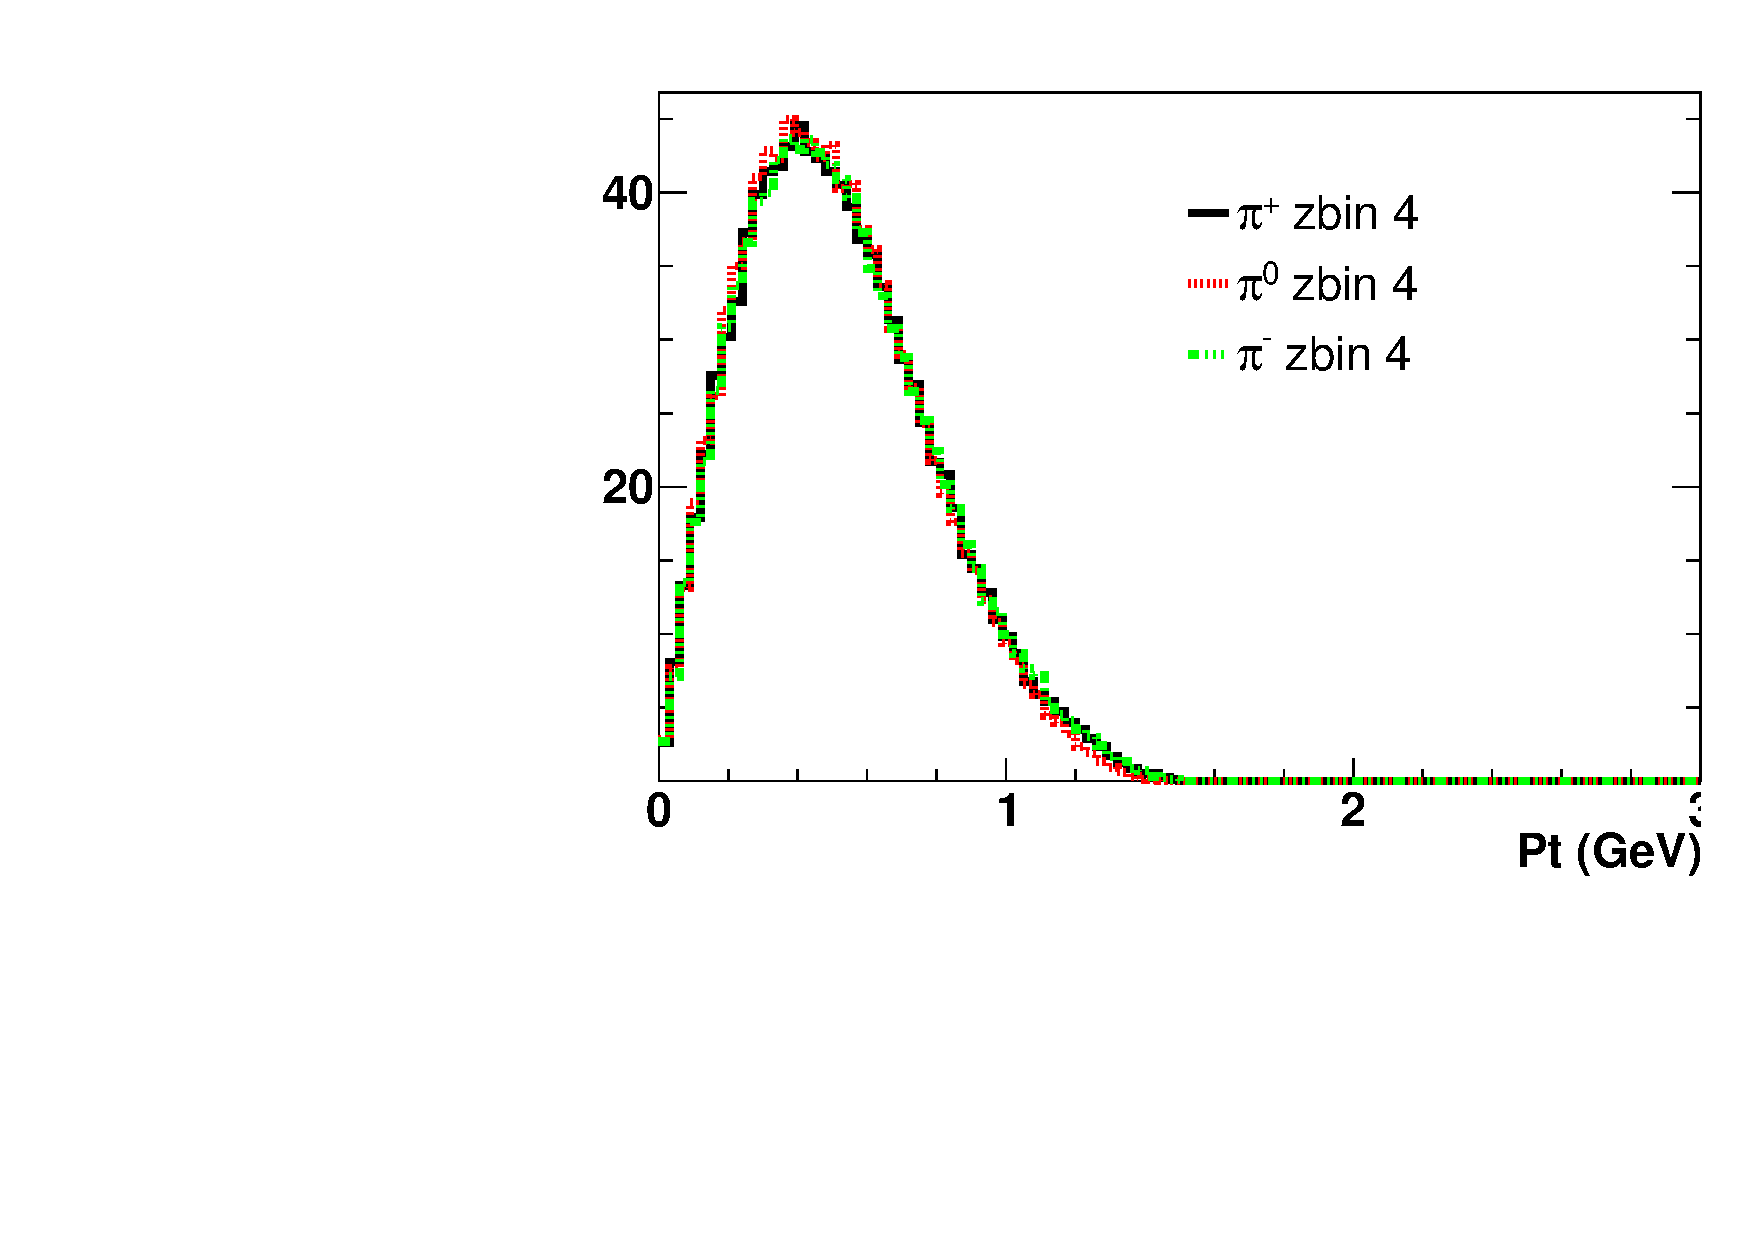
\includegraphics[width=.27\textwidth,natwidth=250,natheight=100]{figure_fiducial/had0.5/Pt_distri_for_zbin_4_norm_had05.pdf}
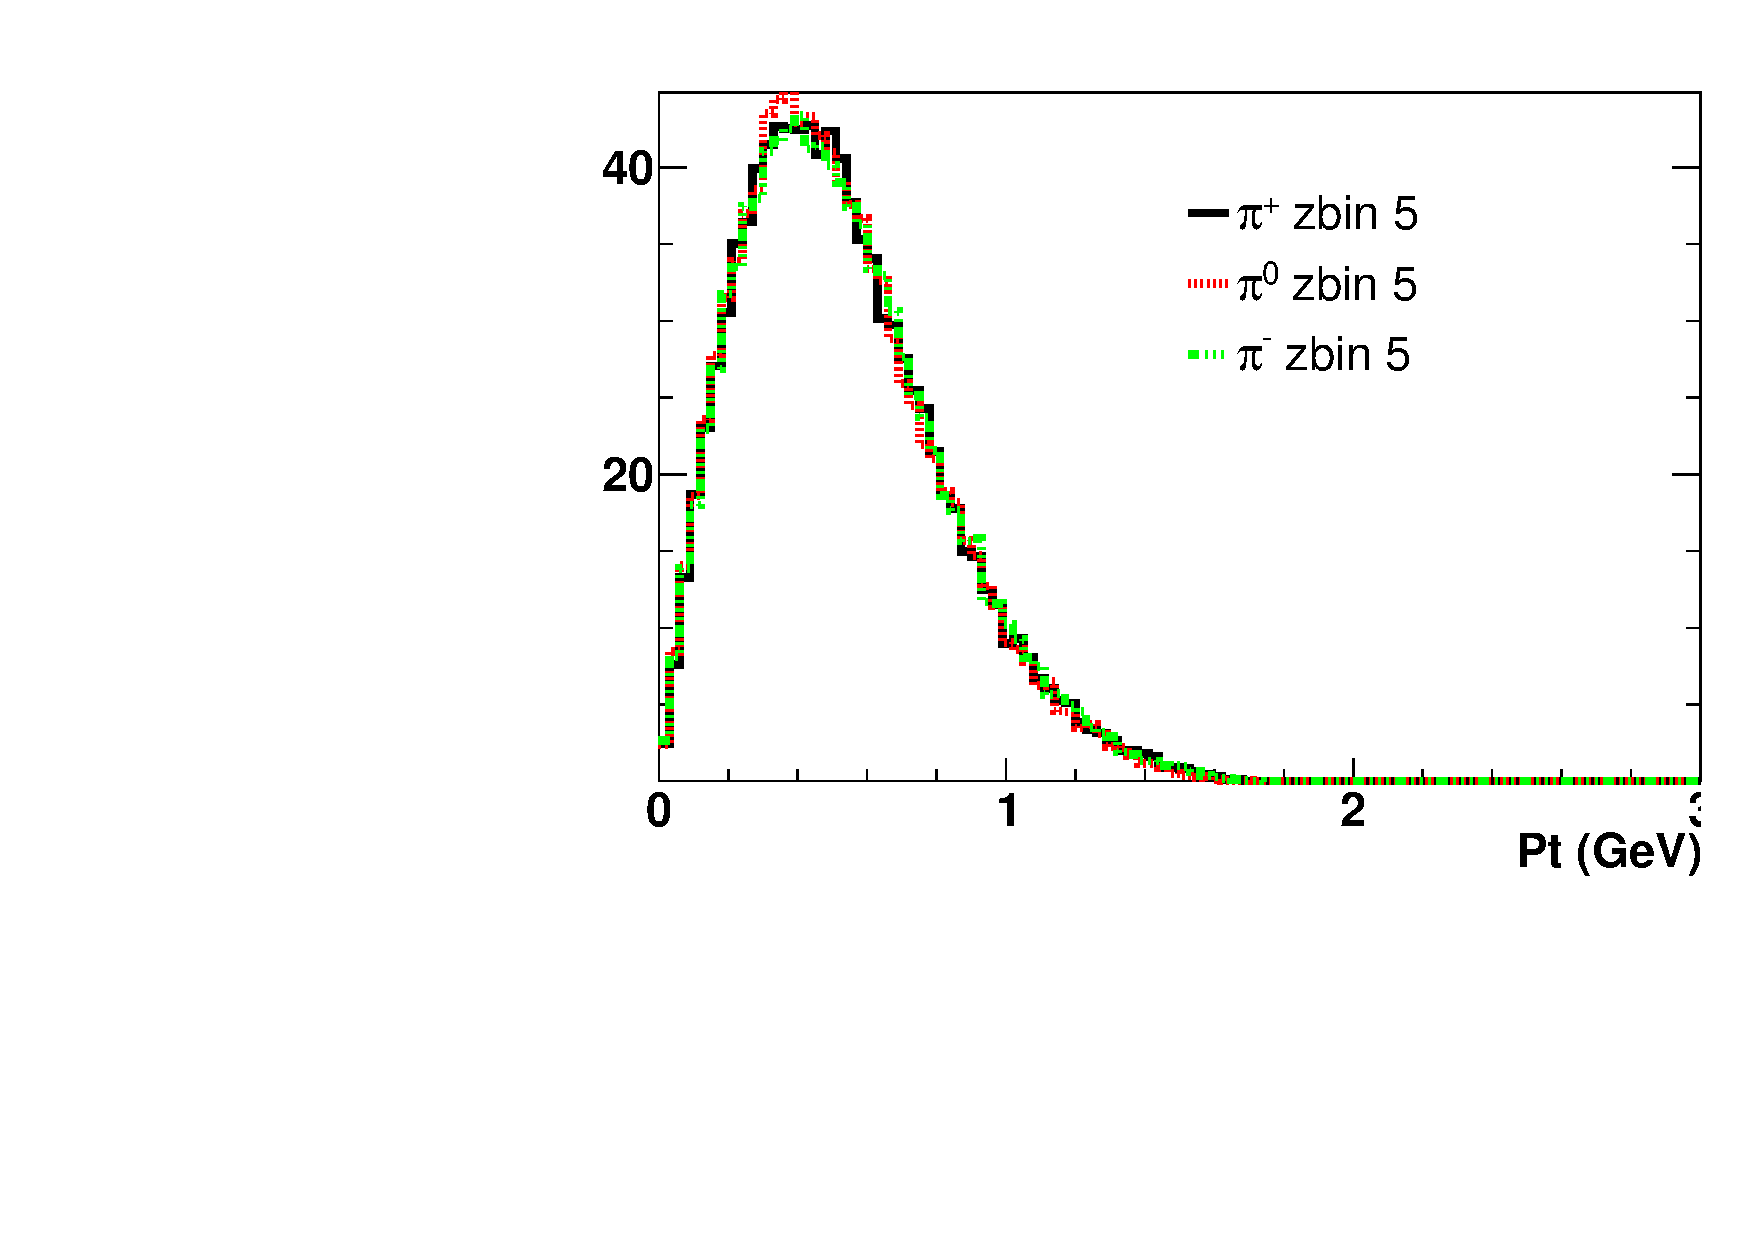
\includegraphics[width=.27\textwidth,natwidth=250,natheight=100]{figure_fiducial/had0.5/Pt_distri_for_zbin_5_norm_had05.pdf}\hfill
\caption[$P_t$ distribution for pions in the various $z$ bins]{$P_t$ distribution for pions in the various $z$ bins. Hadron-direction constraint for the first and fourth row is $H_{OA}<0.3$, second and fifth row is $H_{OA}<0.4$, third and the last row is $H_{OA}<0.5$.}
\end{figure}

\begin{figure}[H]
\captionsetup[subfloat]{farskip=2pt,captionskip=1pt}
\centering
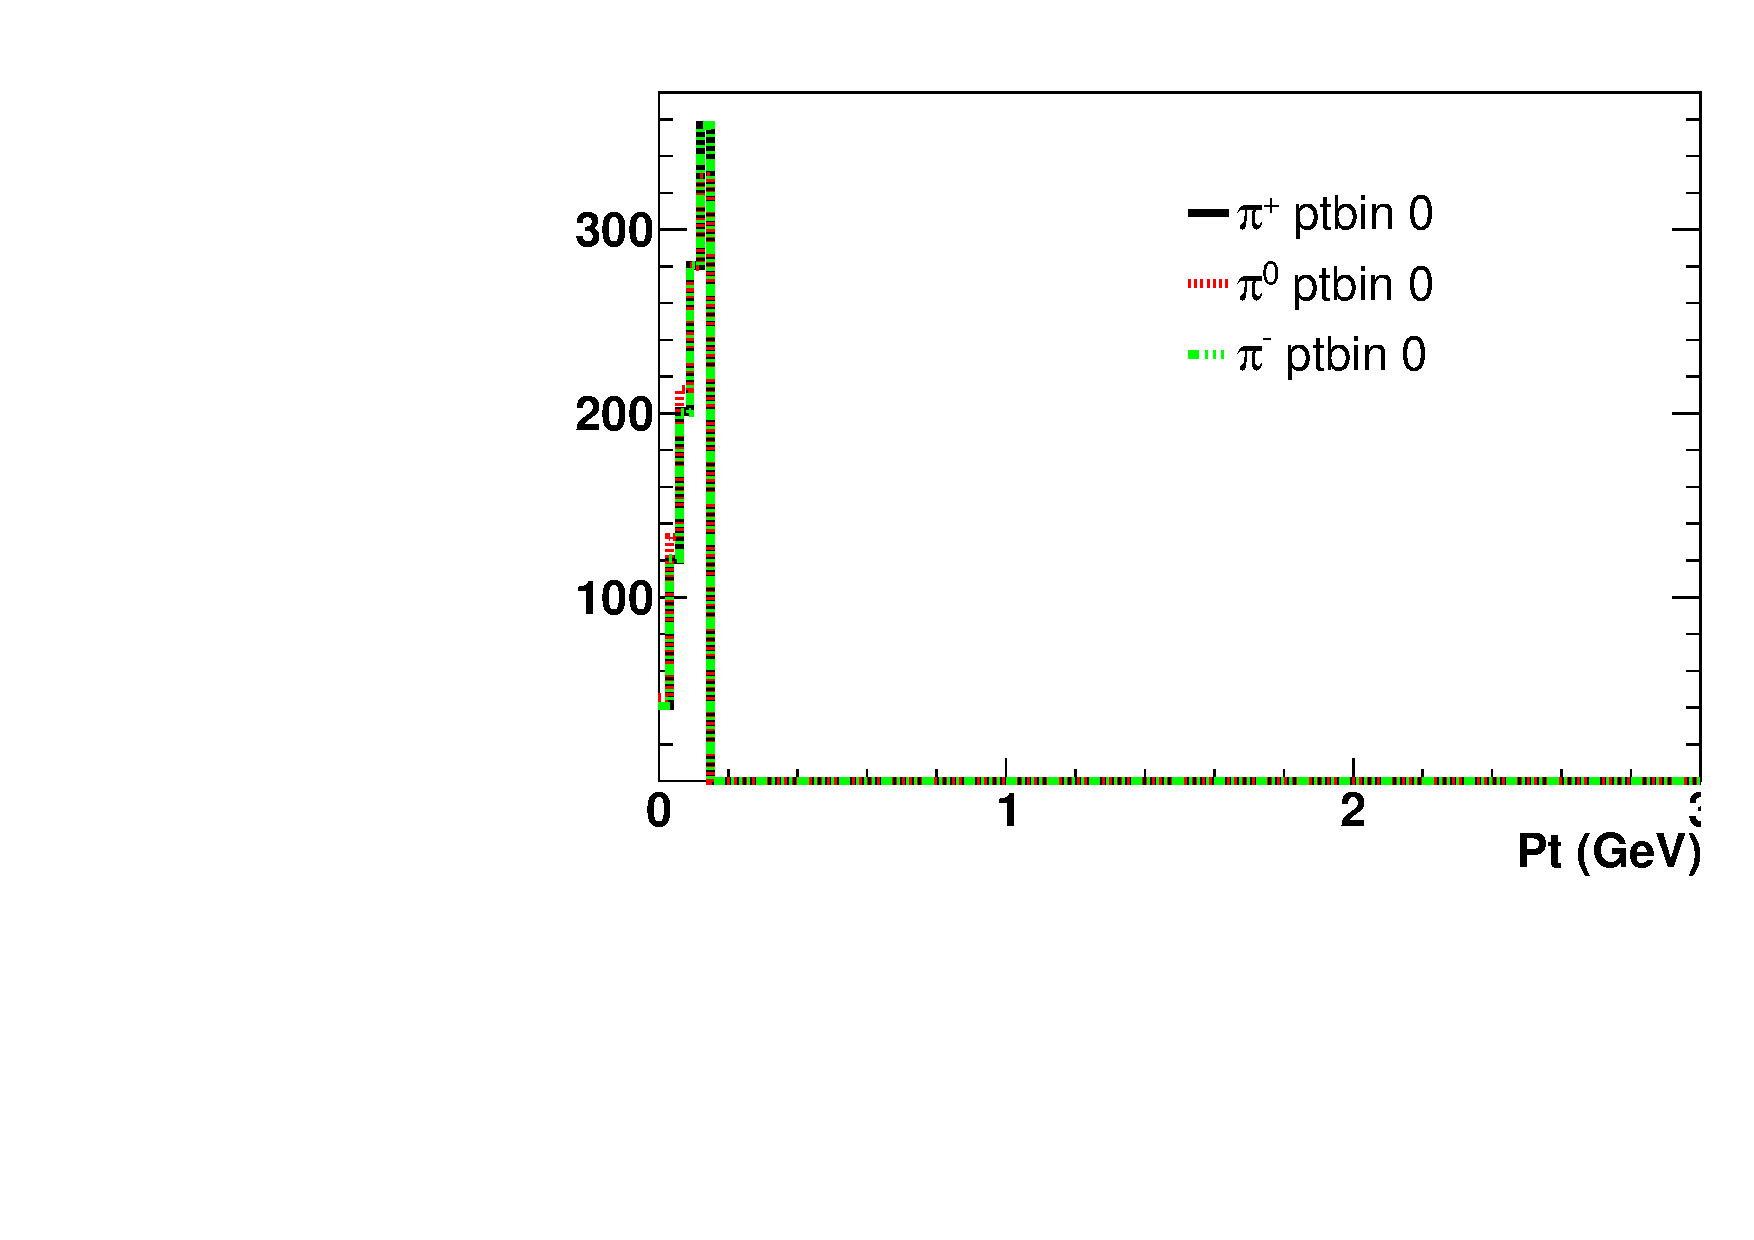
\includegraphics[width=.24\textwidth,natwidth=250,natheight=100]{figure_fiducial/had0.3/Pt_distri_for_ptbin_0_norm_had03.pdf}
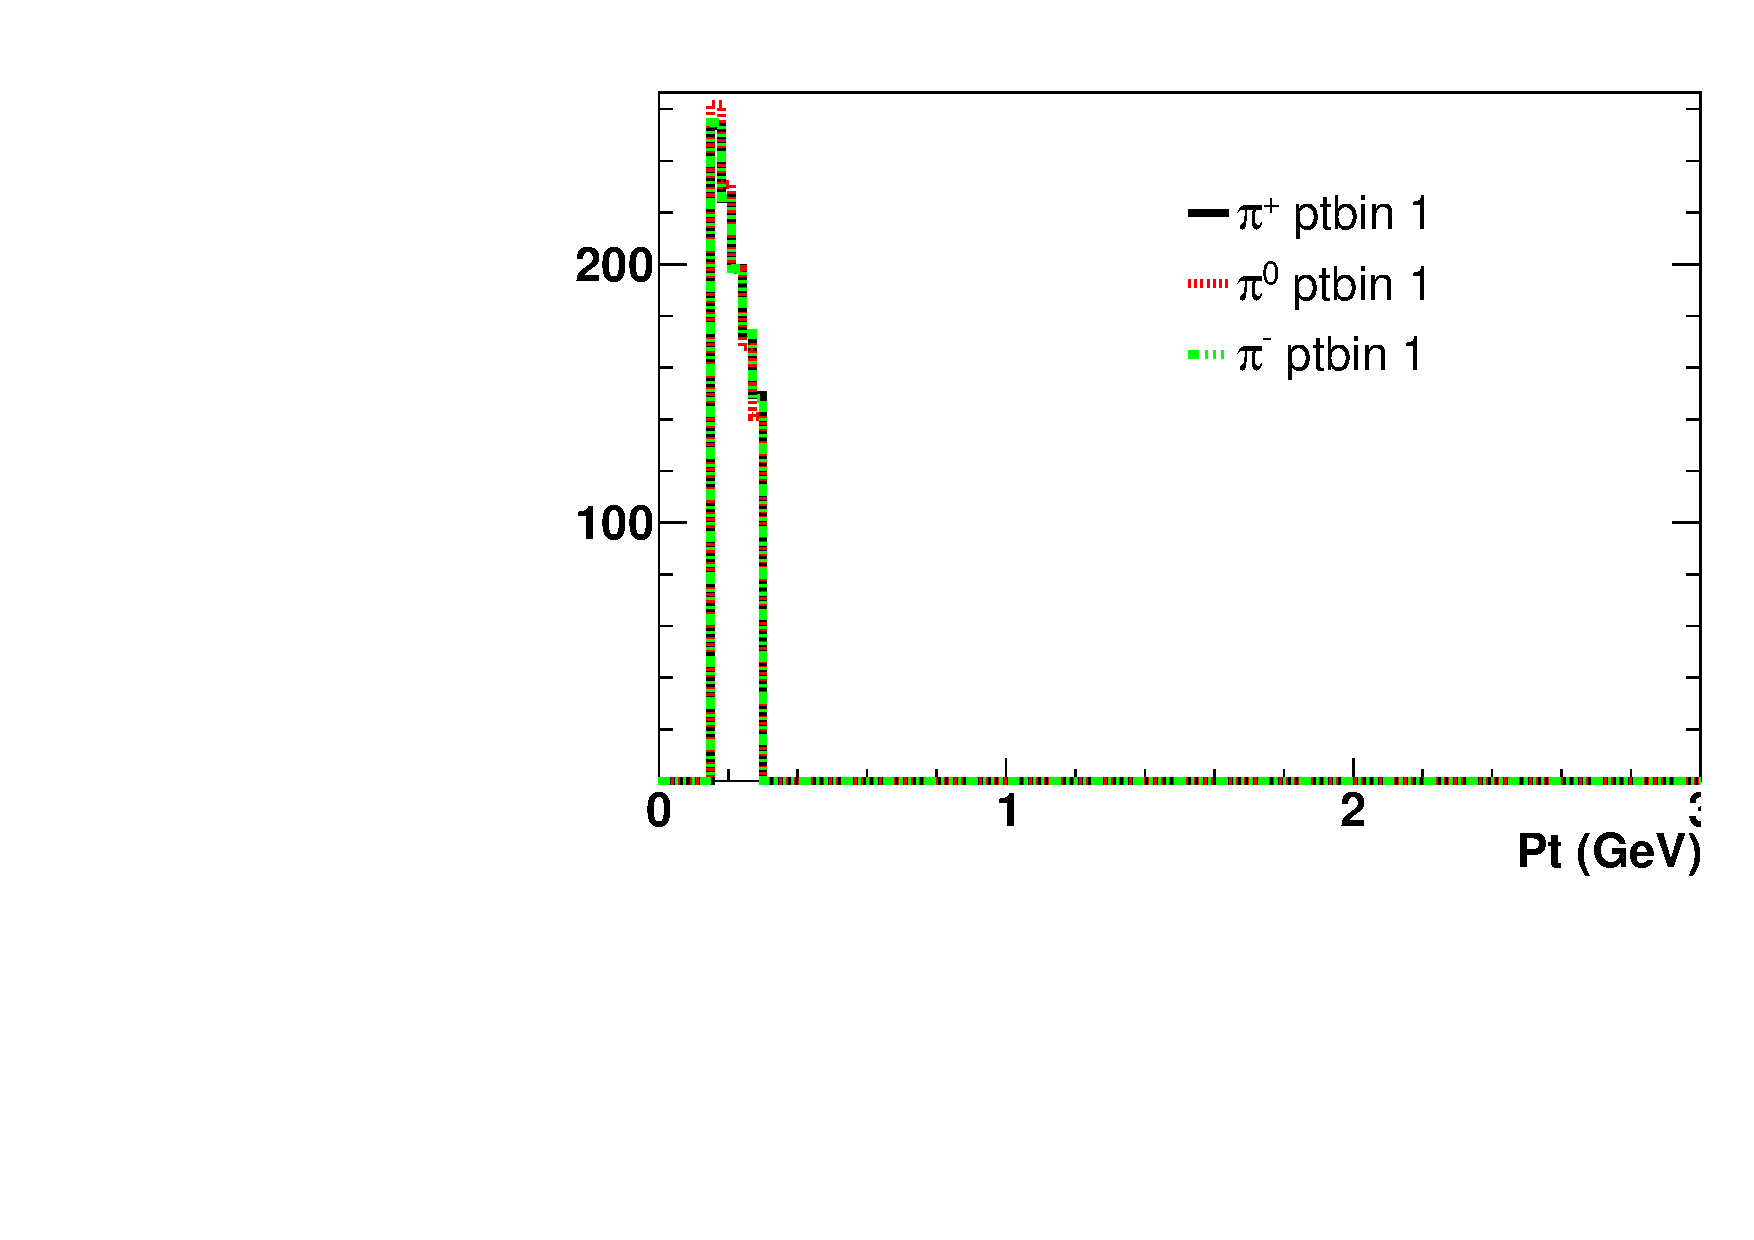
\includegraphics[width=.24\textwidth,natwidth=250,natheight=100]{figure_fiducial/had0.3/Pt_distri_for_ptbin_1_norm_had03.pdf}
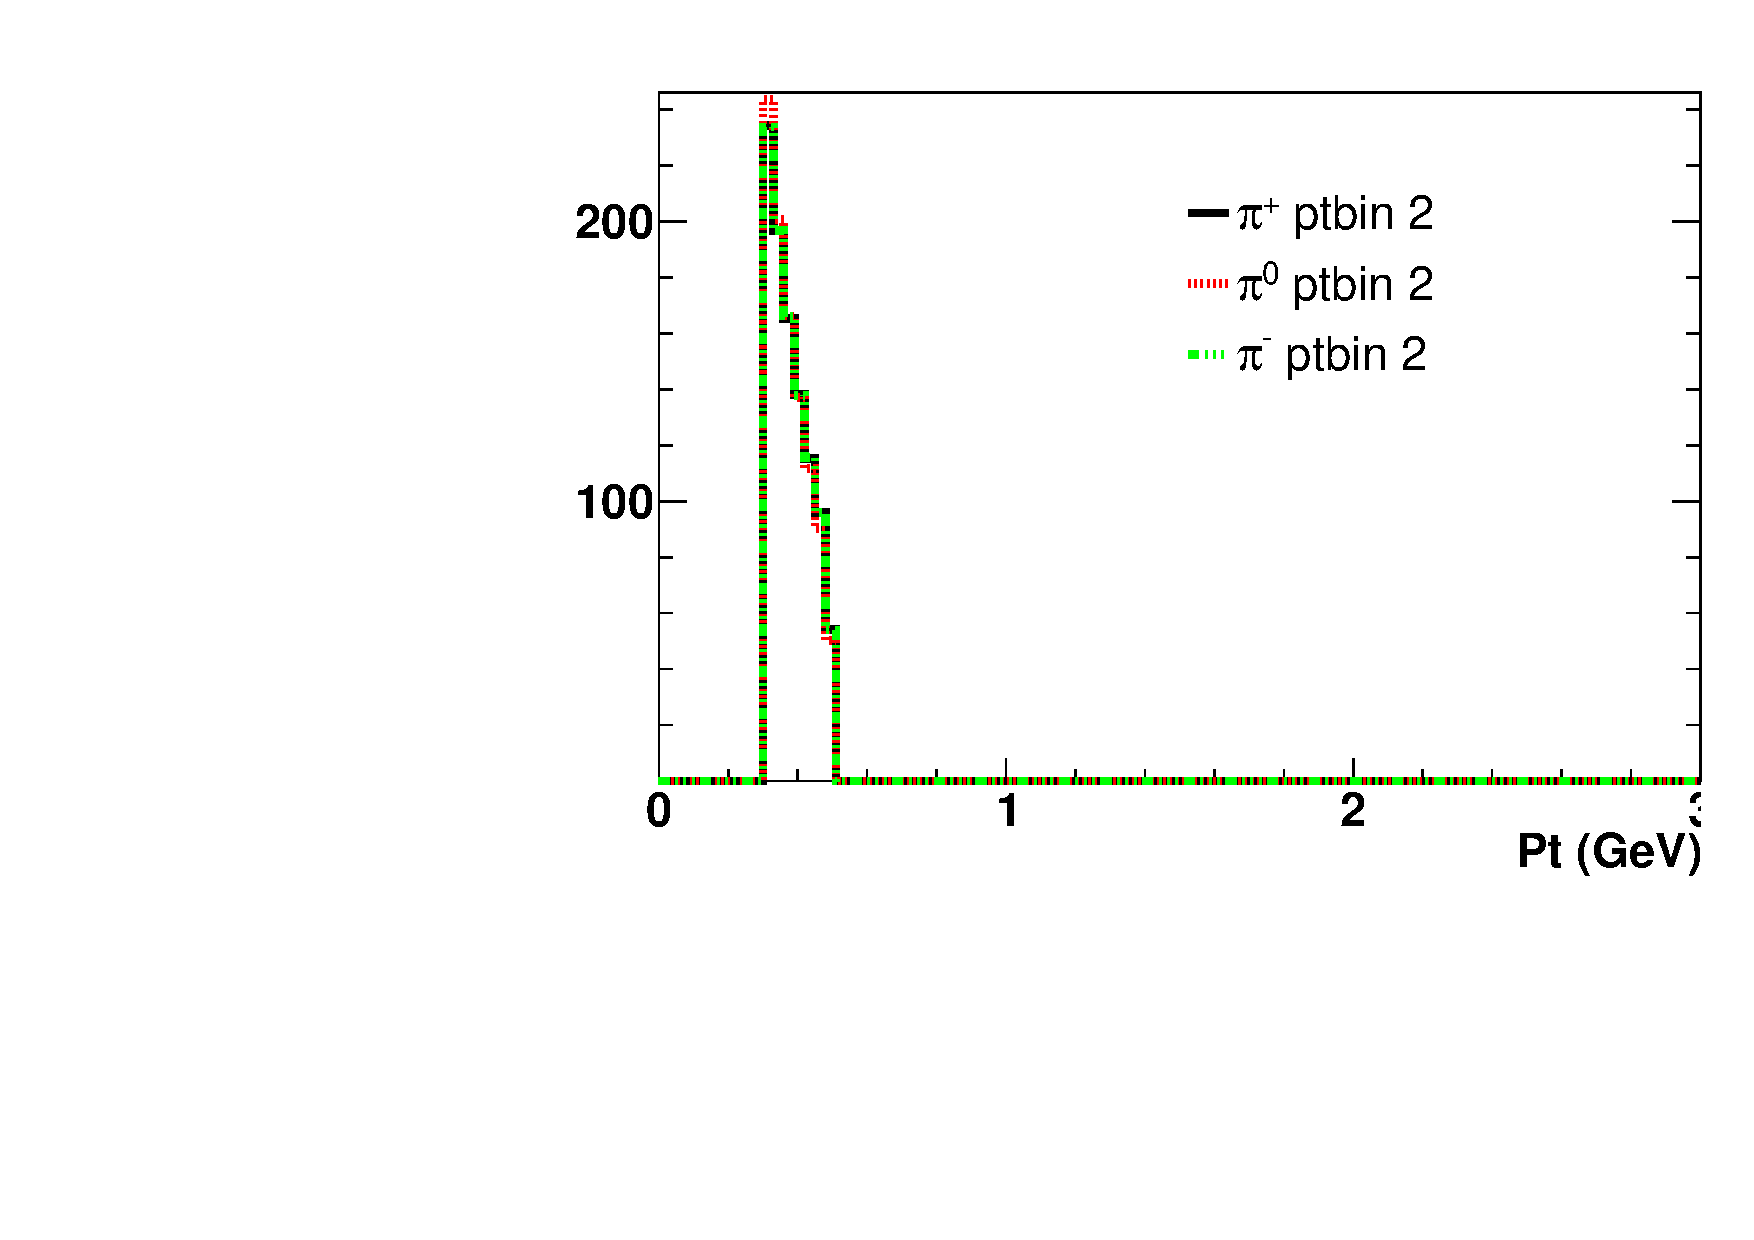
\includegraphics[width=.24\textwidth,natwidth=250,natheight=100]{figure_fiducial/had0.3/Pt_distri_for_ptbin_2_norm_had03.pdf}
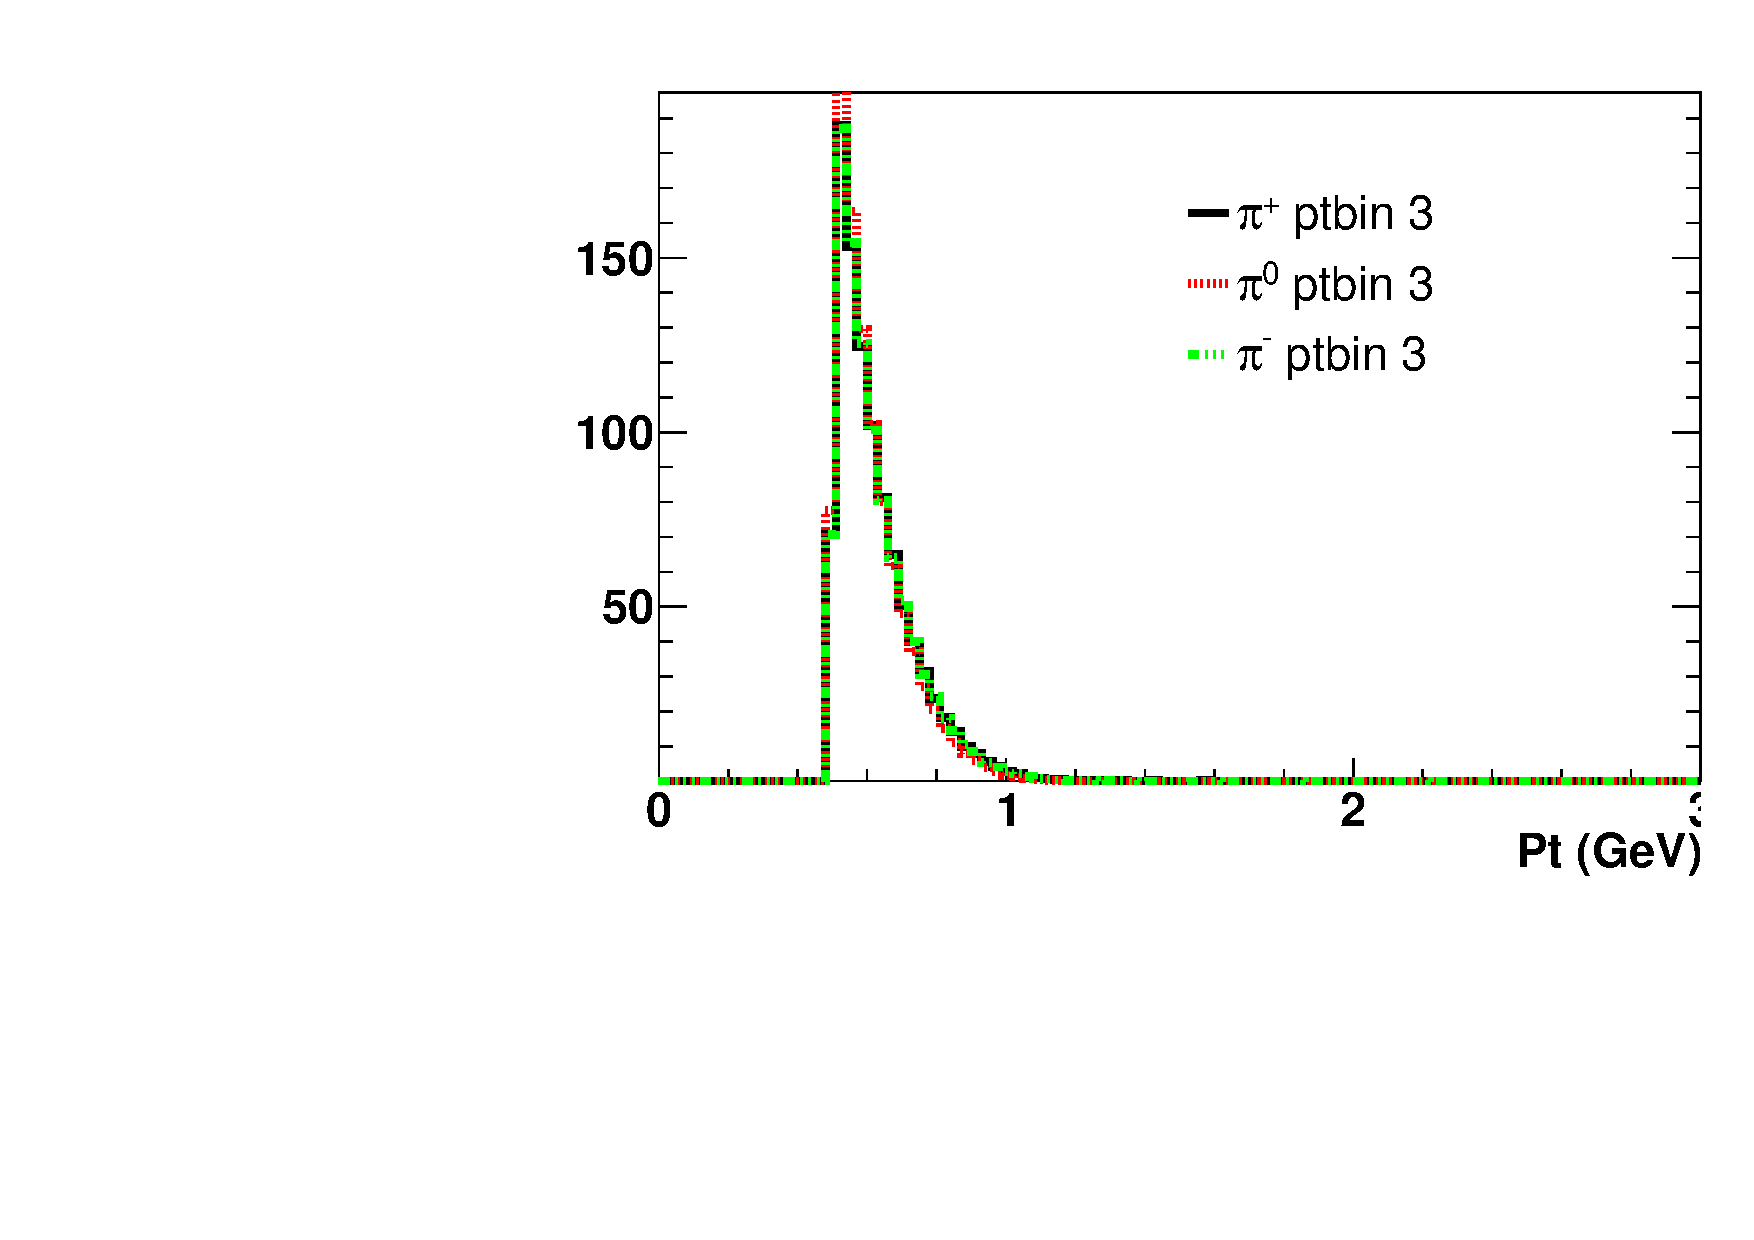
\includegraphics[width=.24\textwidth,natwidth=250,natheight=100]{figure_fiducial/had0.3/Pt_distri_for_ptbin_3_norm_had03.pdf}\hfill
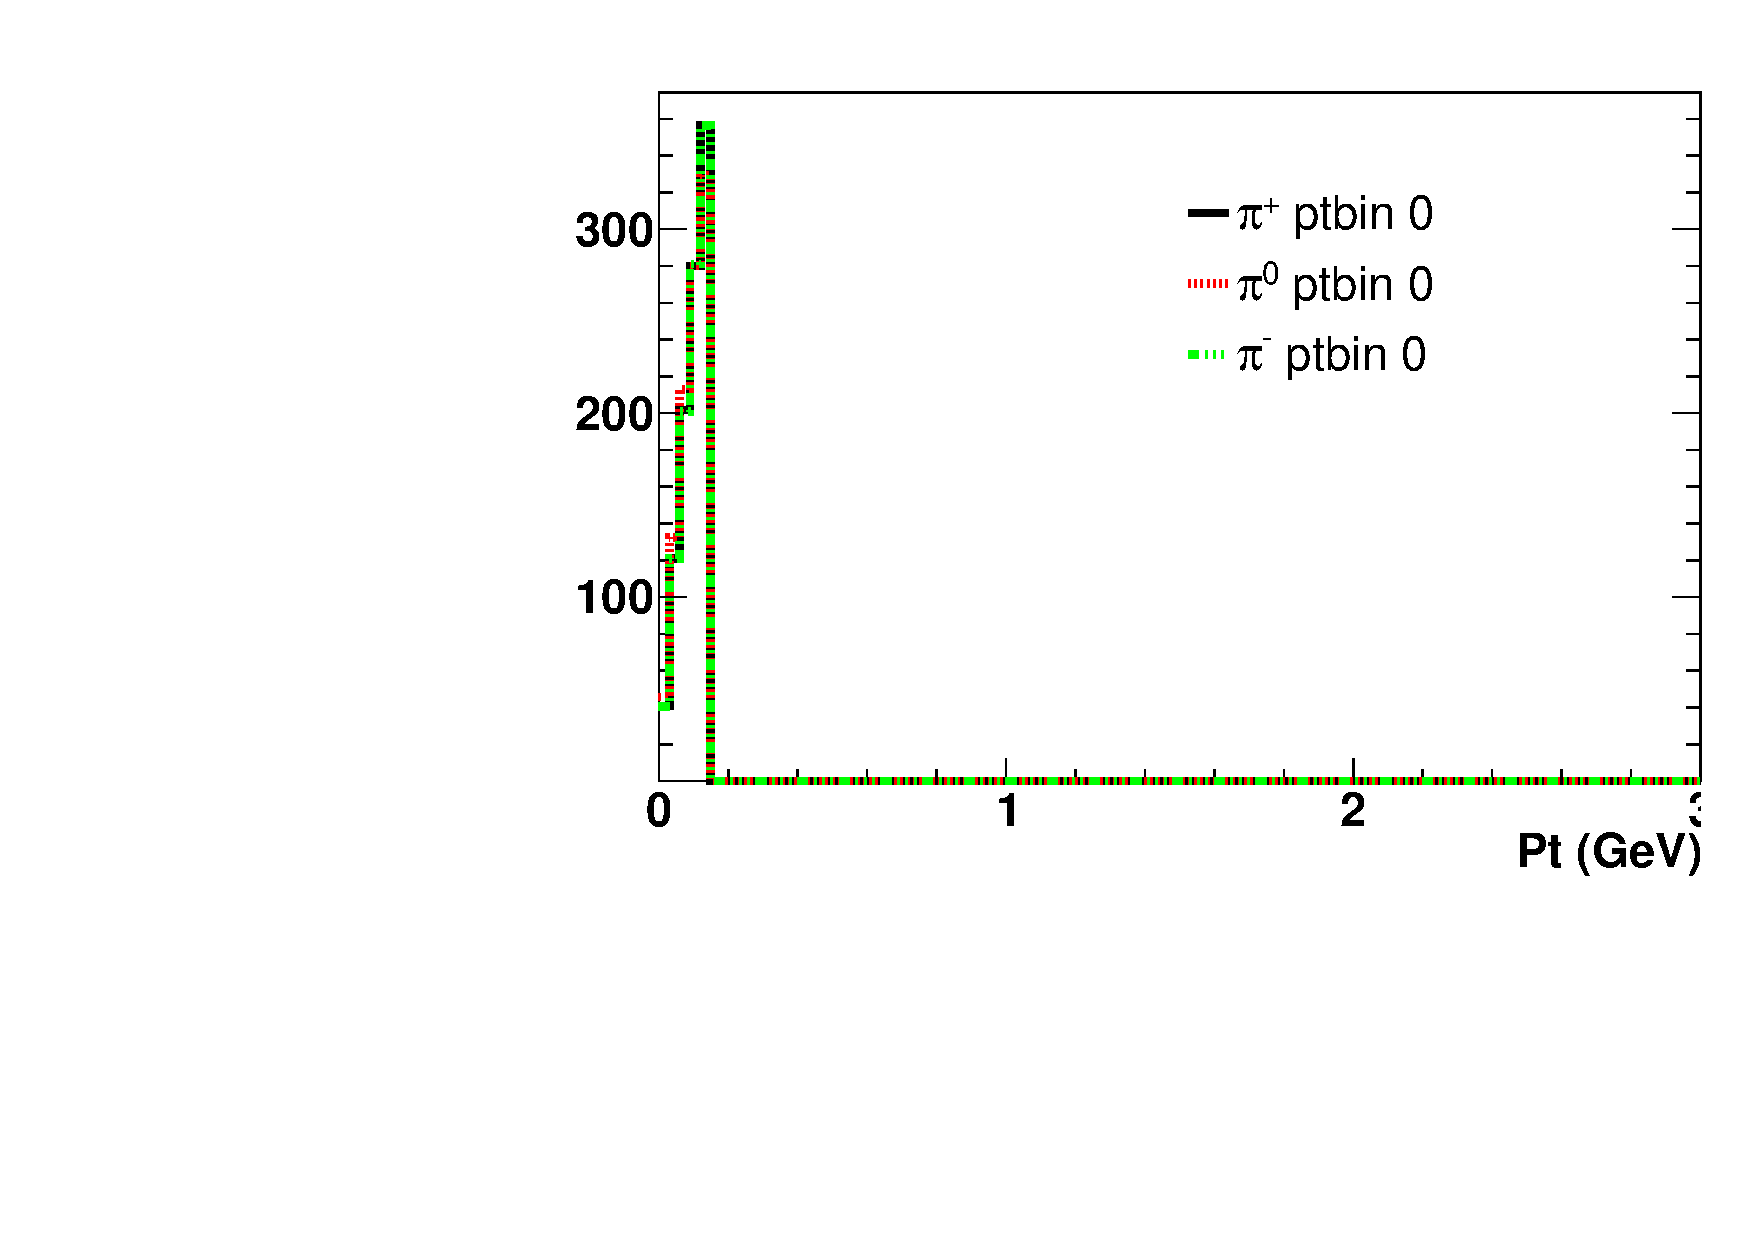
\includegraphics[width=.24\textwidth,natwidth=250,natheight=100]{figure_fiducial/had0.4/Pt_distri_for_ptbin_0_norm_had04.pdf}
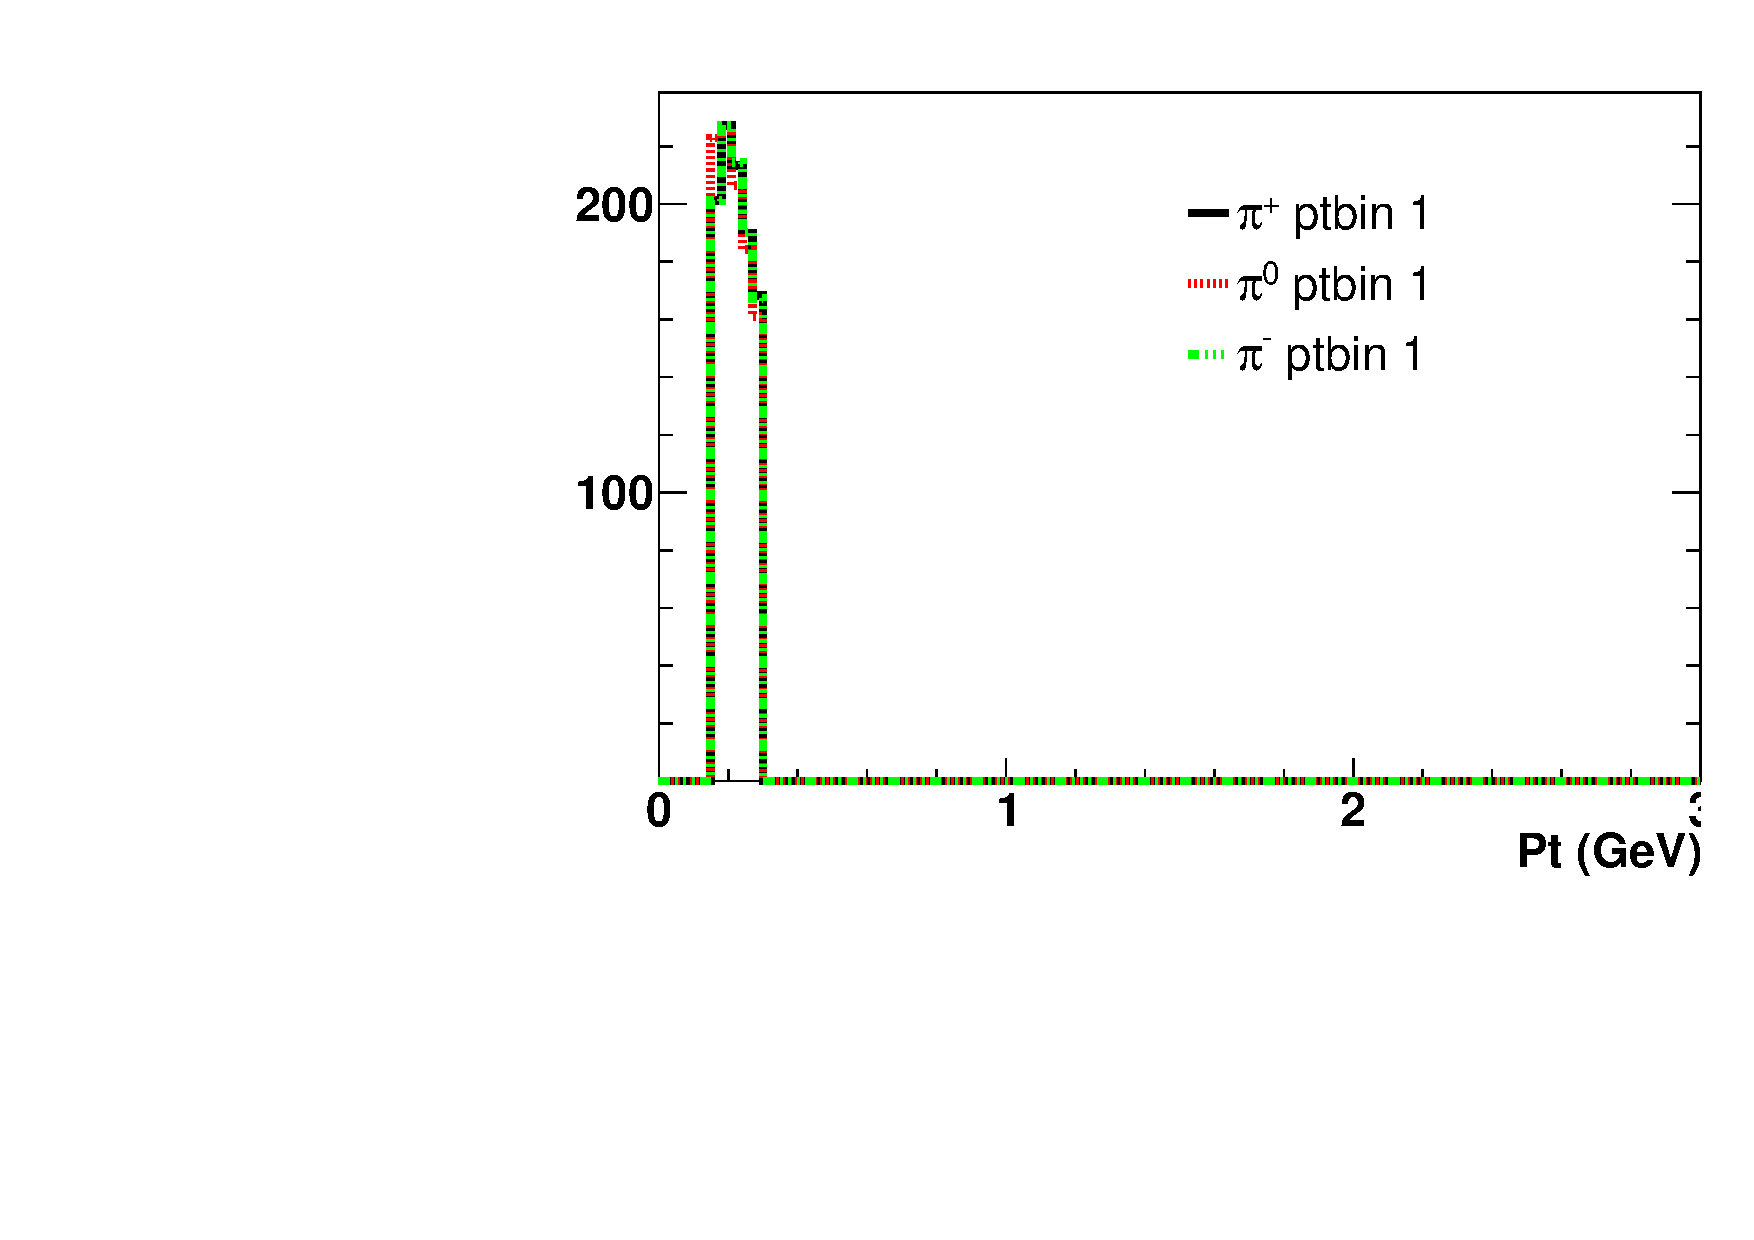
\includegraphics[width=.24\textwidth,natwidth=250,natheight=100]{figure_fiducial/had0.4/Pt_distri_for_ptbin_1_norm_had04.pdf}
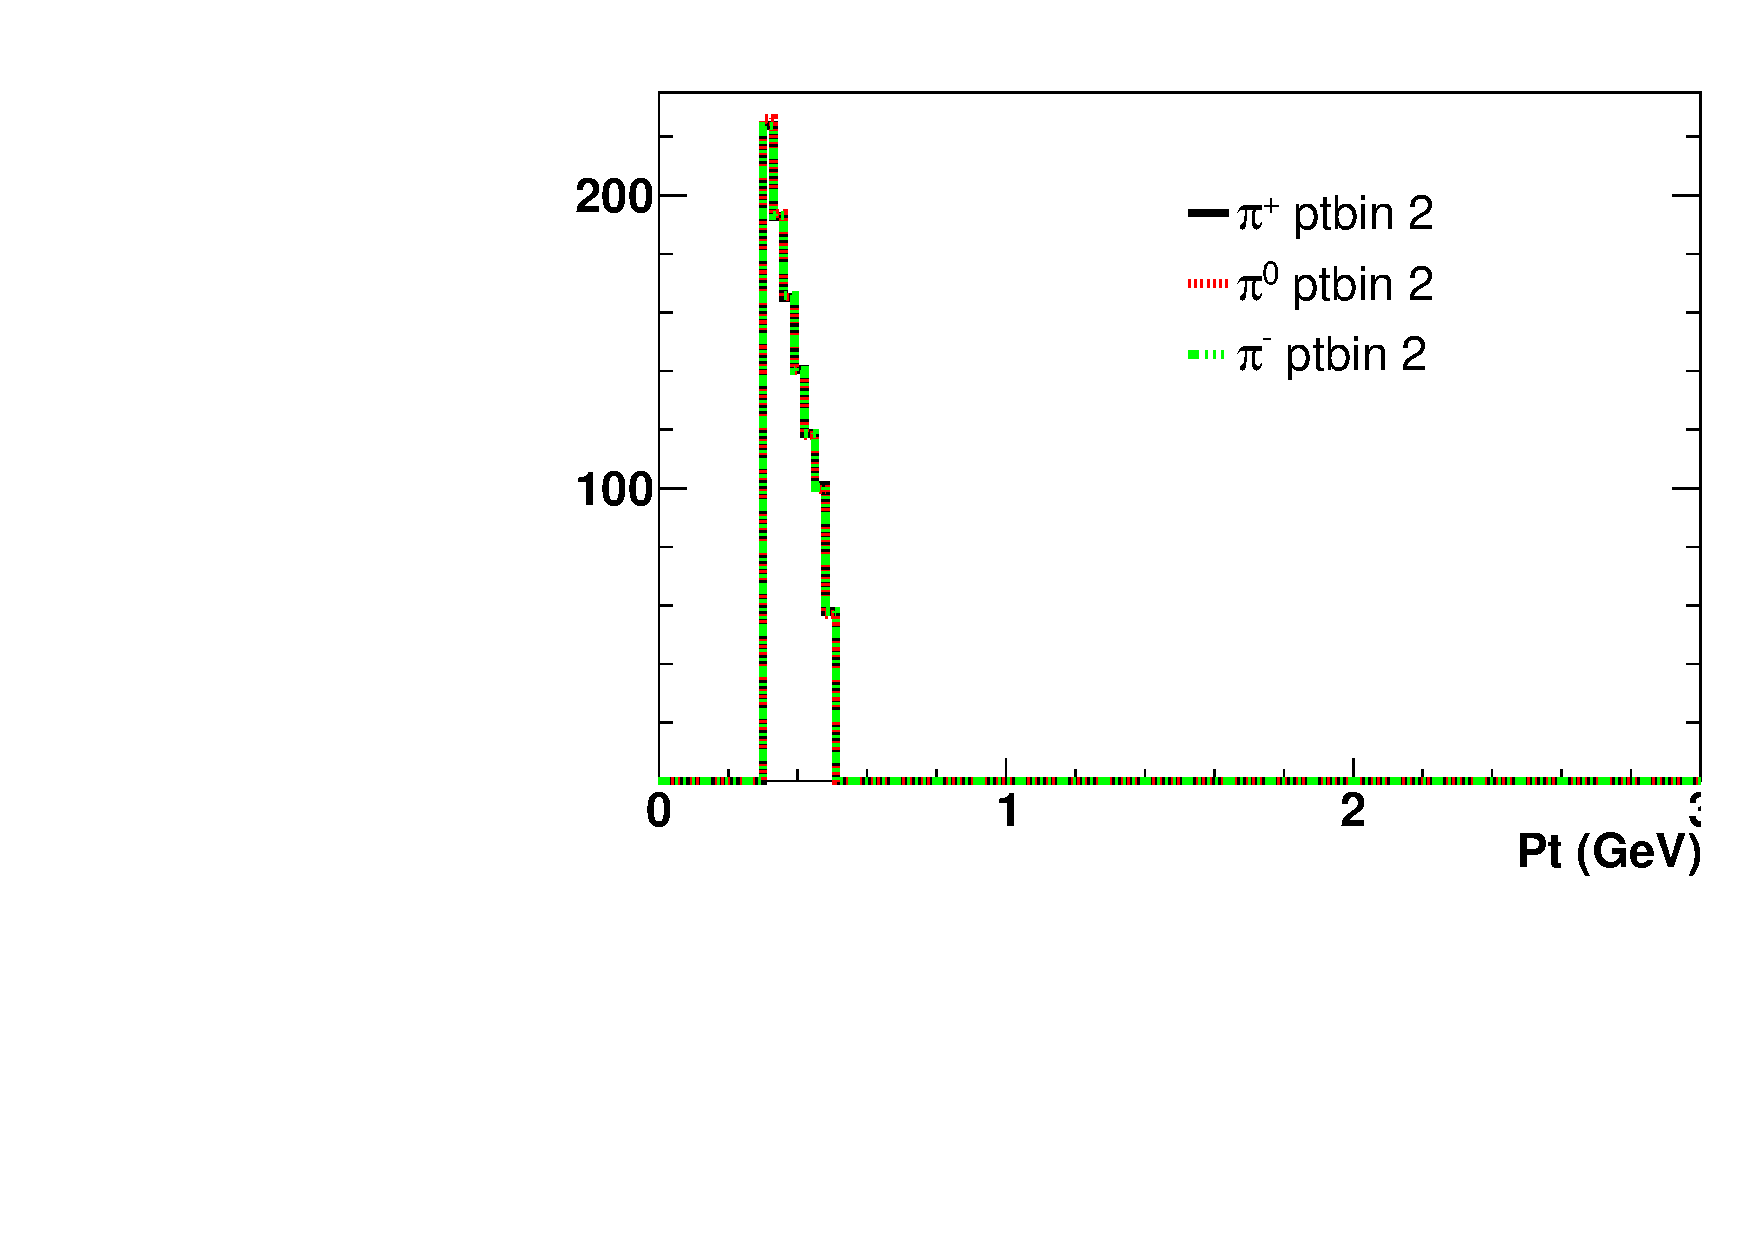
\includegraphics[width=.24\textwidth,natwidth=250,natheight=100]{figure_fiducial/had0.4/Pt_distri_for_ptbin_2_norm_had04.pdf}
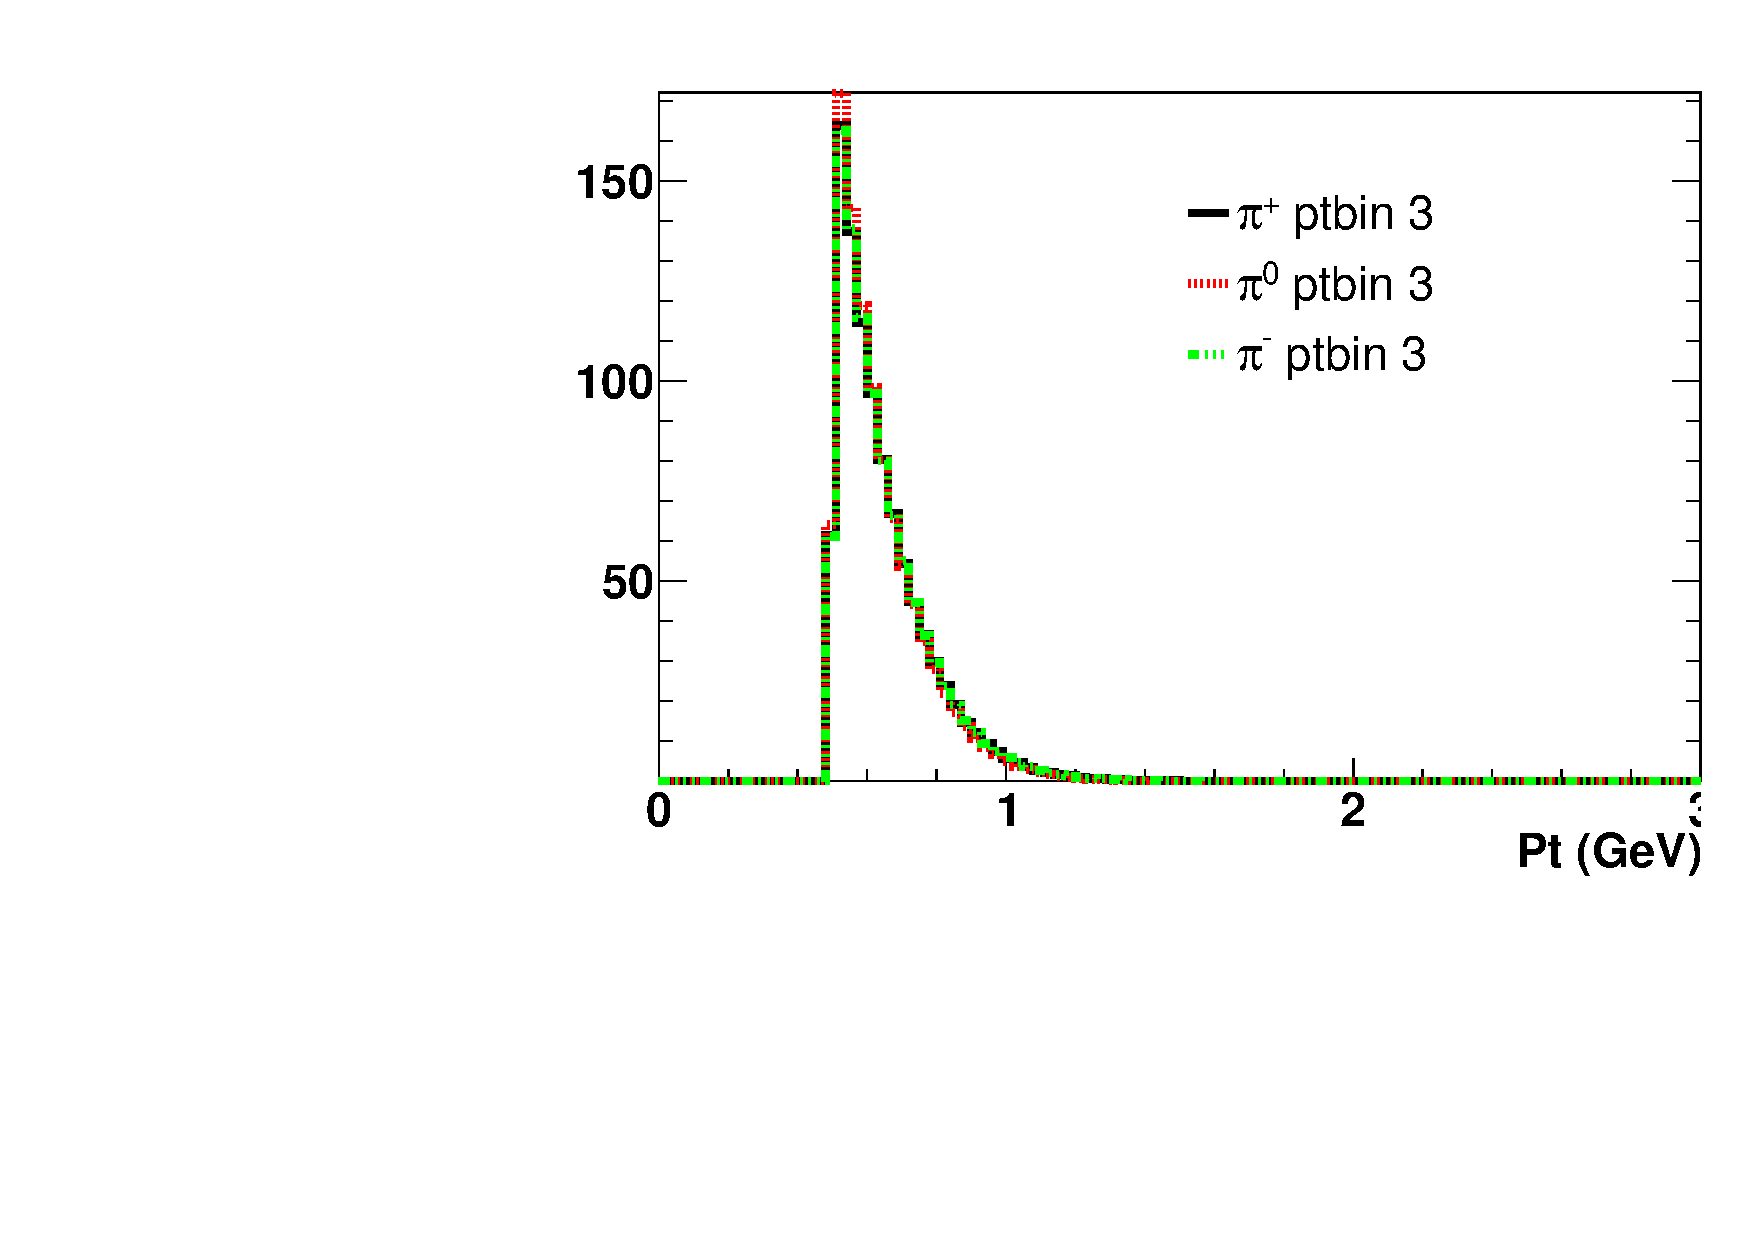
\includegraphics[width=.24\textwidth,natwidth=250,natheight=100]{figure_fiducial/had0.4/Pt_distri_for_ptbin_3_norm_had04.pdf}\hfill
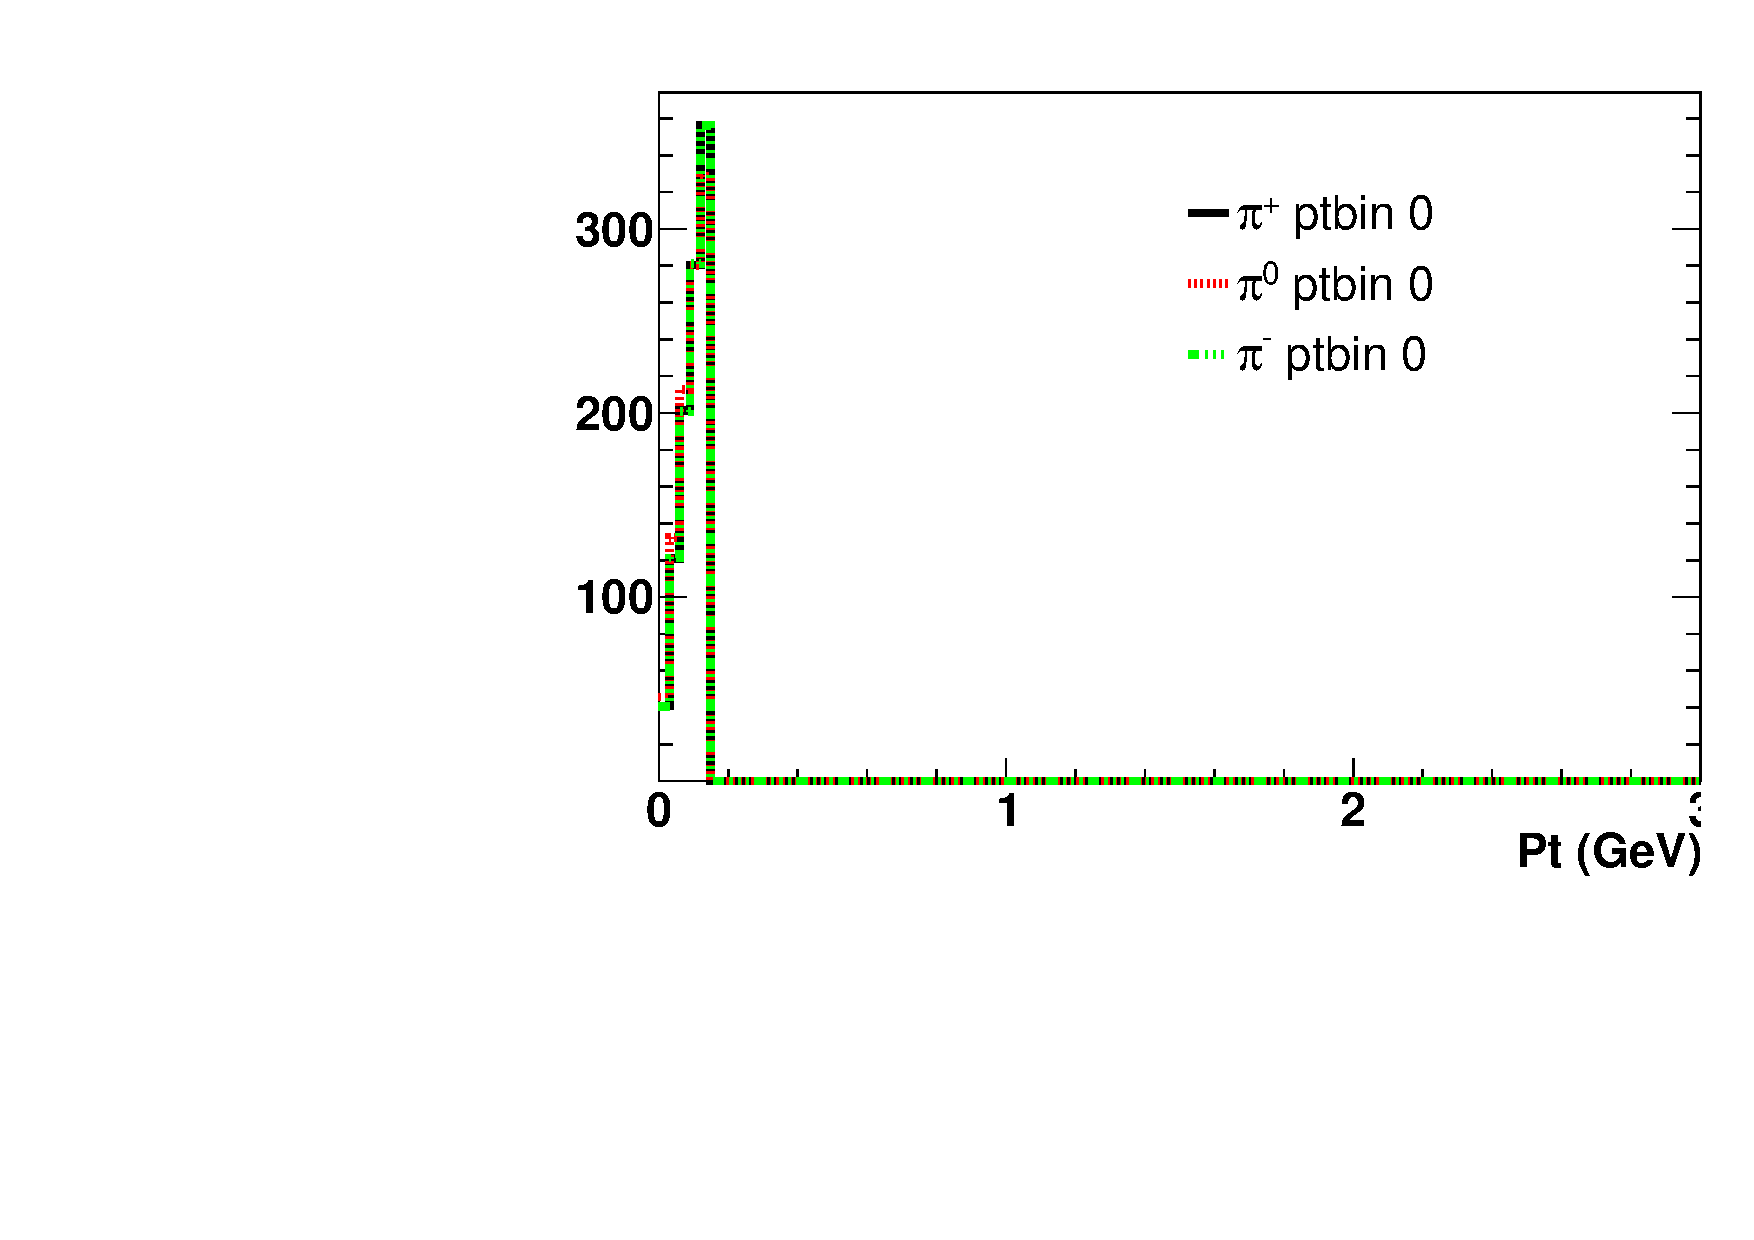
\includegraphics[width=.24\textwidth,natwidth=250,natheight=100]{figure_fiducial/had0.5/Pt_distri_for_ptbin_0_norm_had05.pdf}
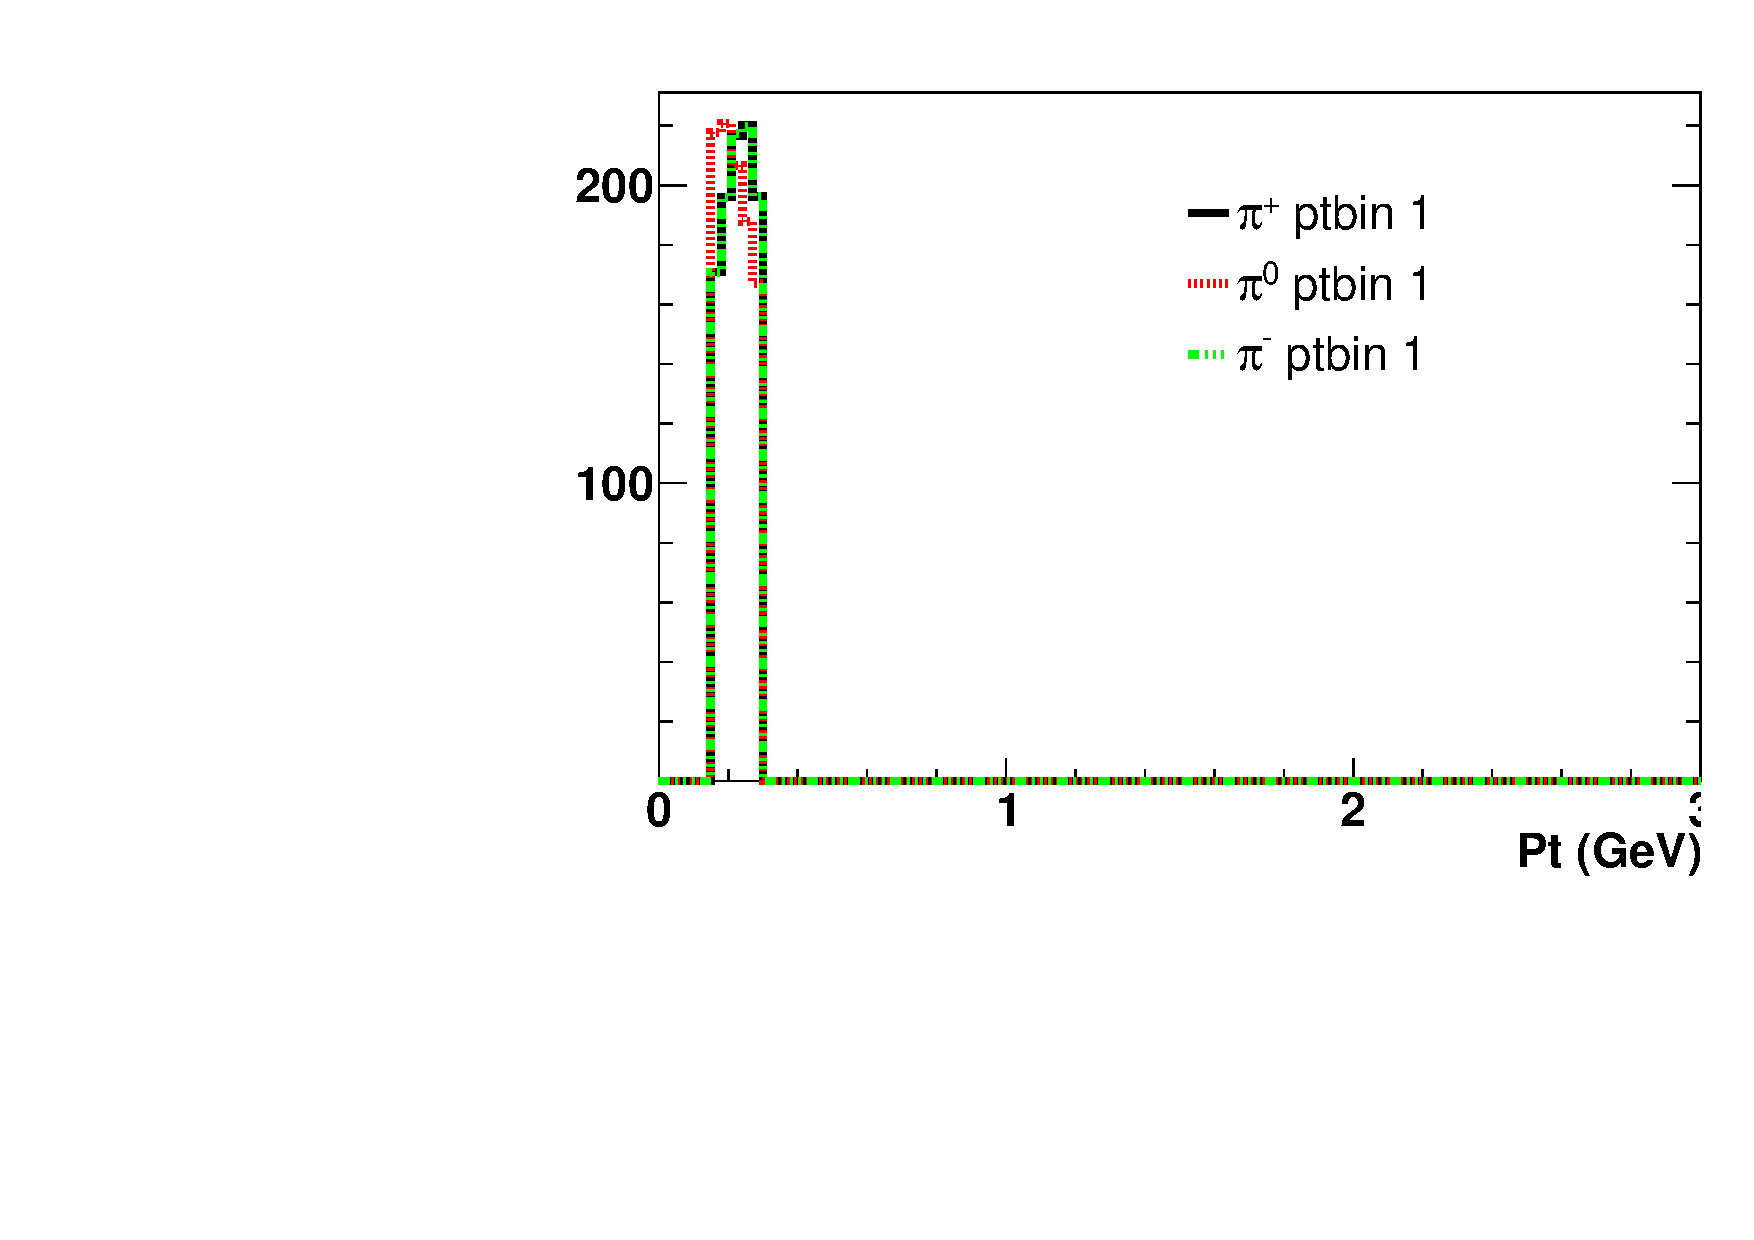
\includegraphics[width=.24\textwidth,natwidth=250,natheight=100]{figure_fiducial/had0.5/Pt_distri_for_ptbin_1_norm_had05.pdf}
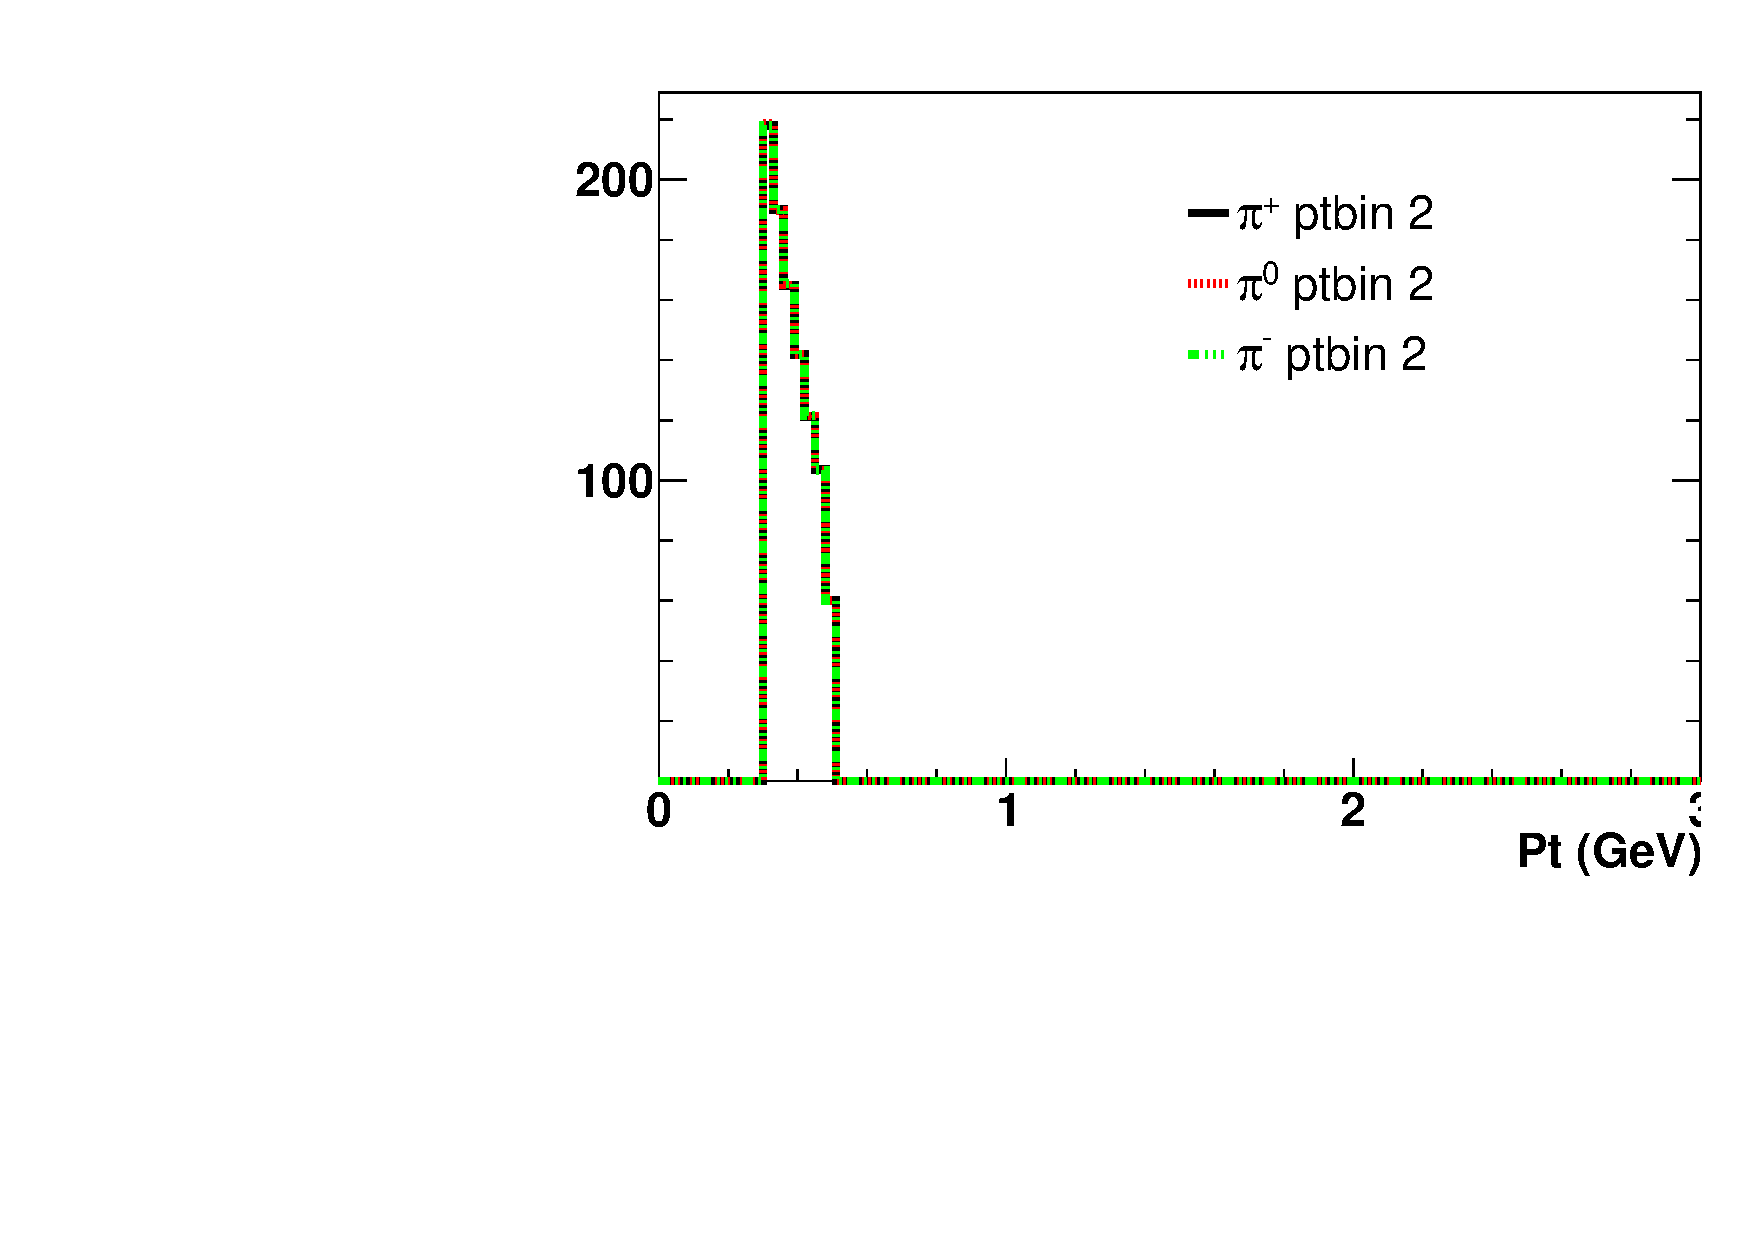
\includegraphics[width=.24\textwidth,natwidth=250,natheight=100]{figure_fiducial/had0.5/Pt_distri_for_ptbin_2_norm_had05.pdf}
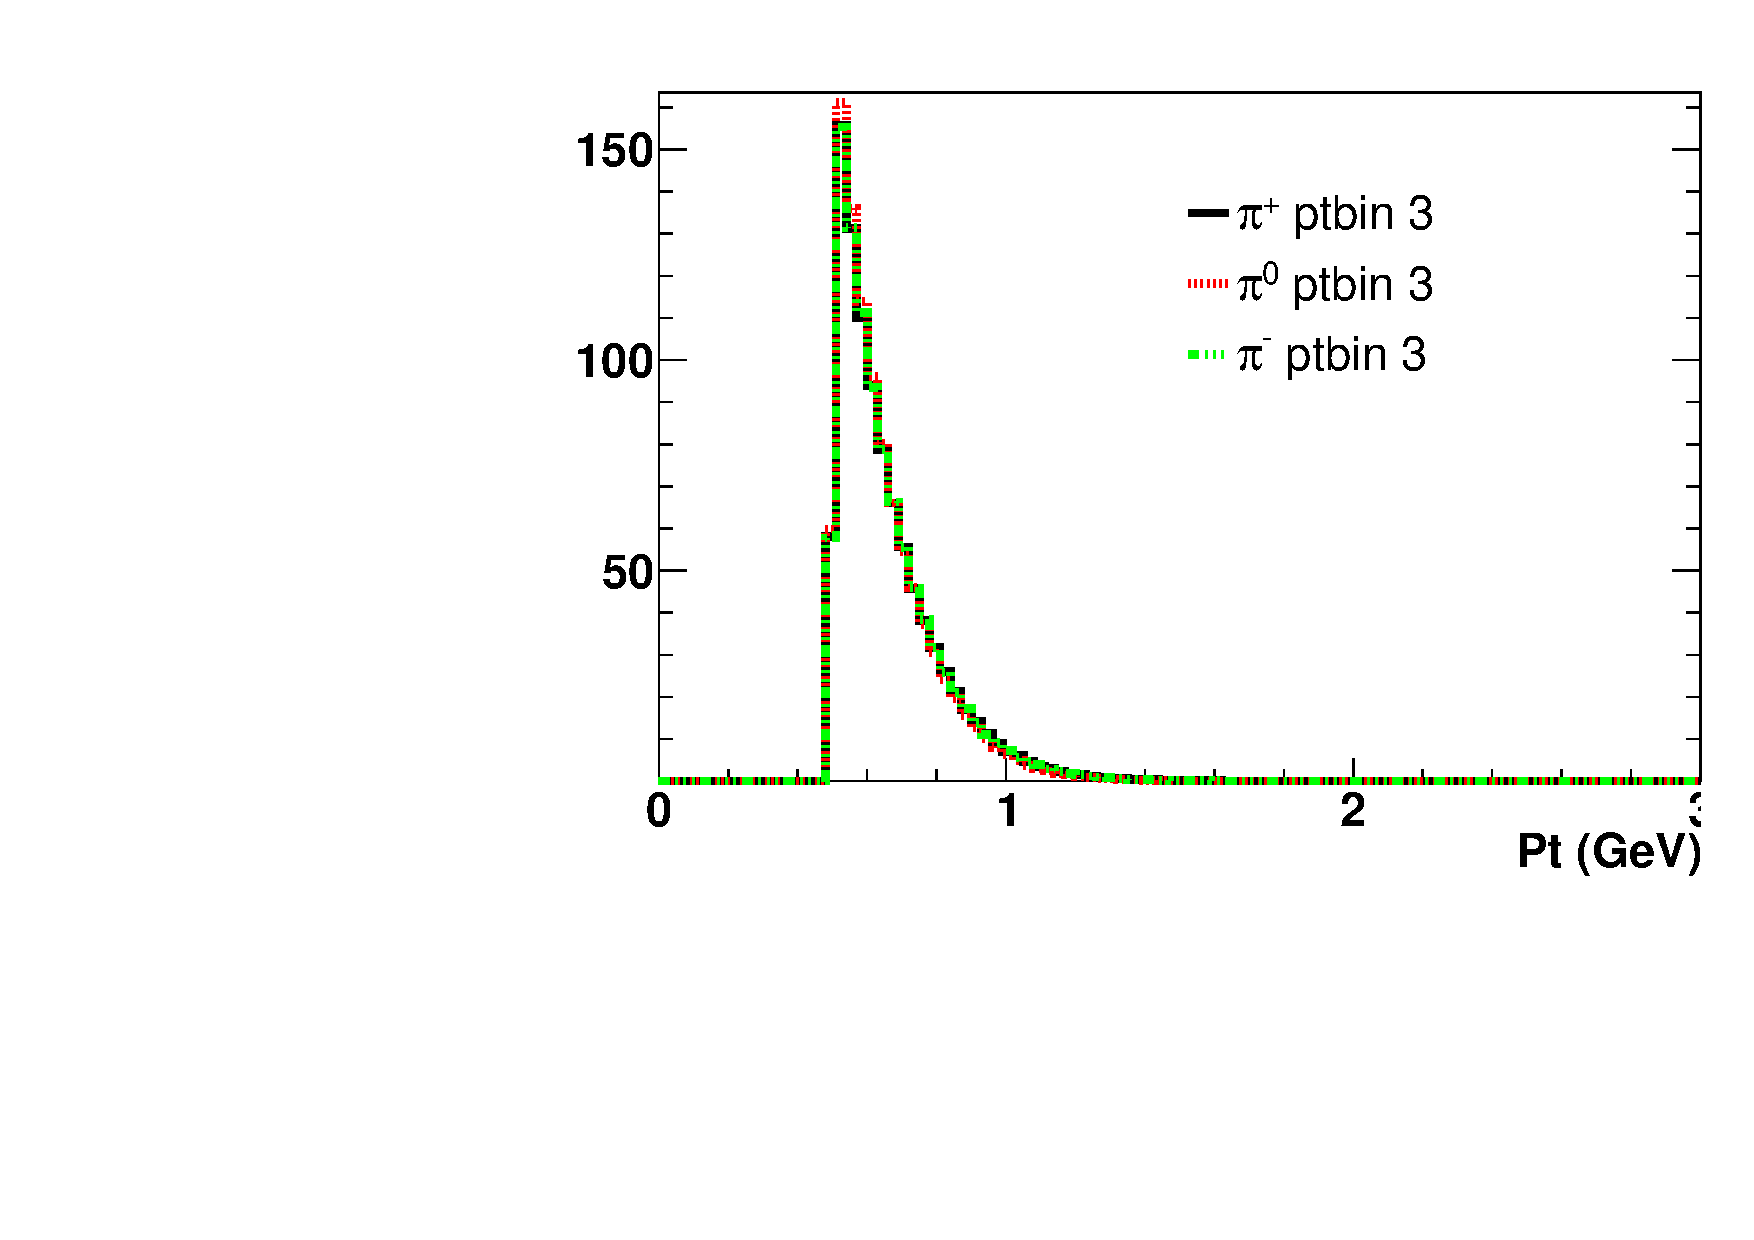
\includegraphics[width=.24\textwidth,natwidth=250,natheight=100]{figure_fiducial/had0.5/Pt_distri_for_ptbin_3_norm_had05.pdf}\hfill
\caption[$P_t$ distribution for pions in the various $P_t$ bins]{$P_t$ distribution for pions in the various $P_t$ bins. Hadron-direction constraint for the first row is $H_{OA}<0.3$, second row is $H_{OA}<0.4$ and the last row is $H_{OA}<0.5$.}
\end{figure}

\begin{figure}[H]
\captionsetup[subfloat]{farskip=2pt,captionskip=1pt}
\centering
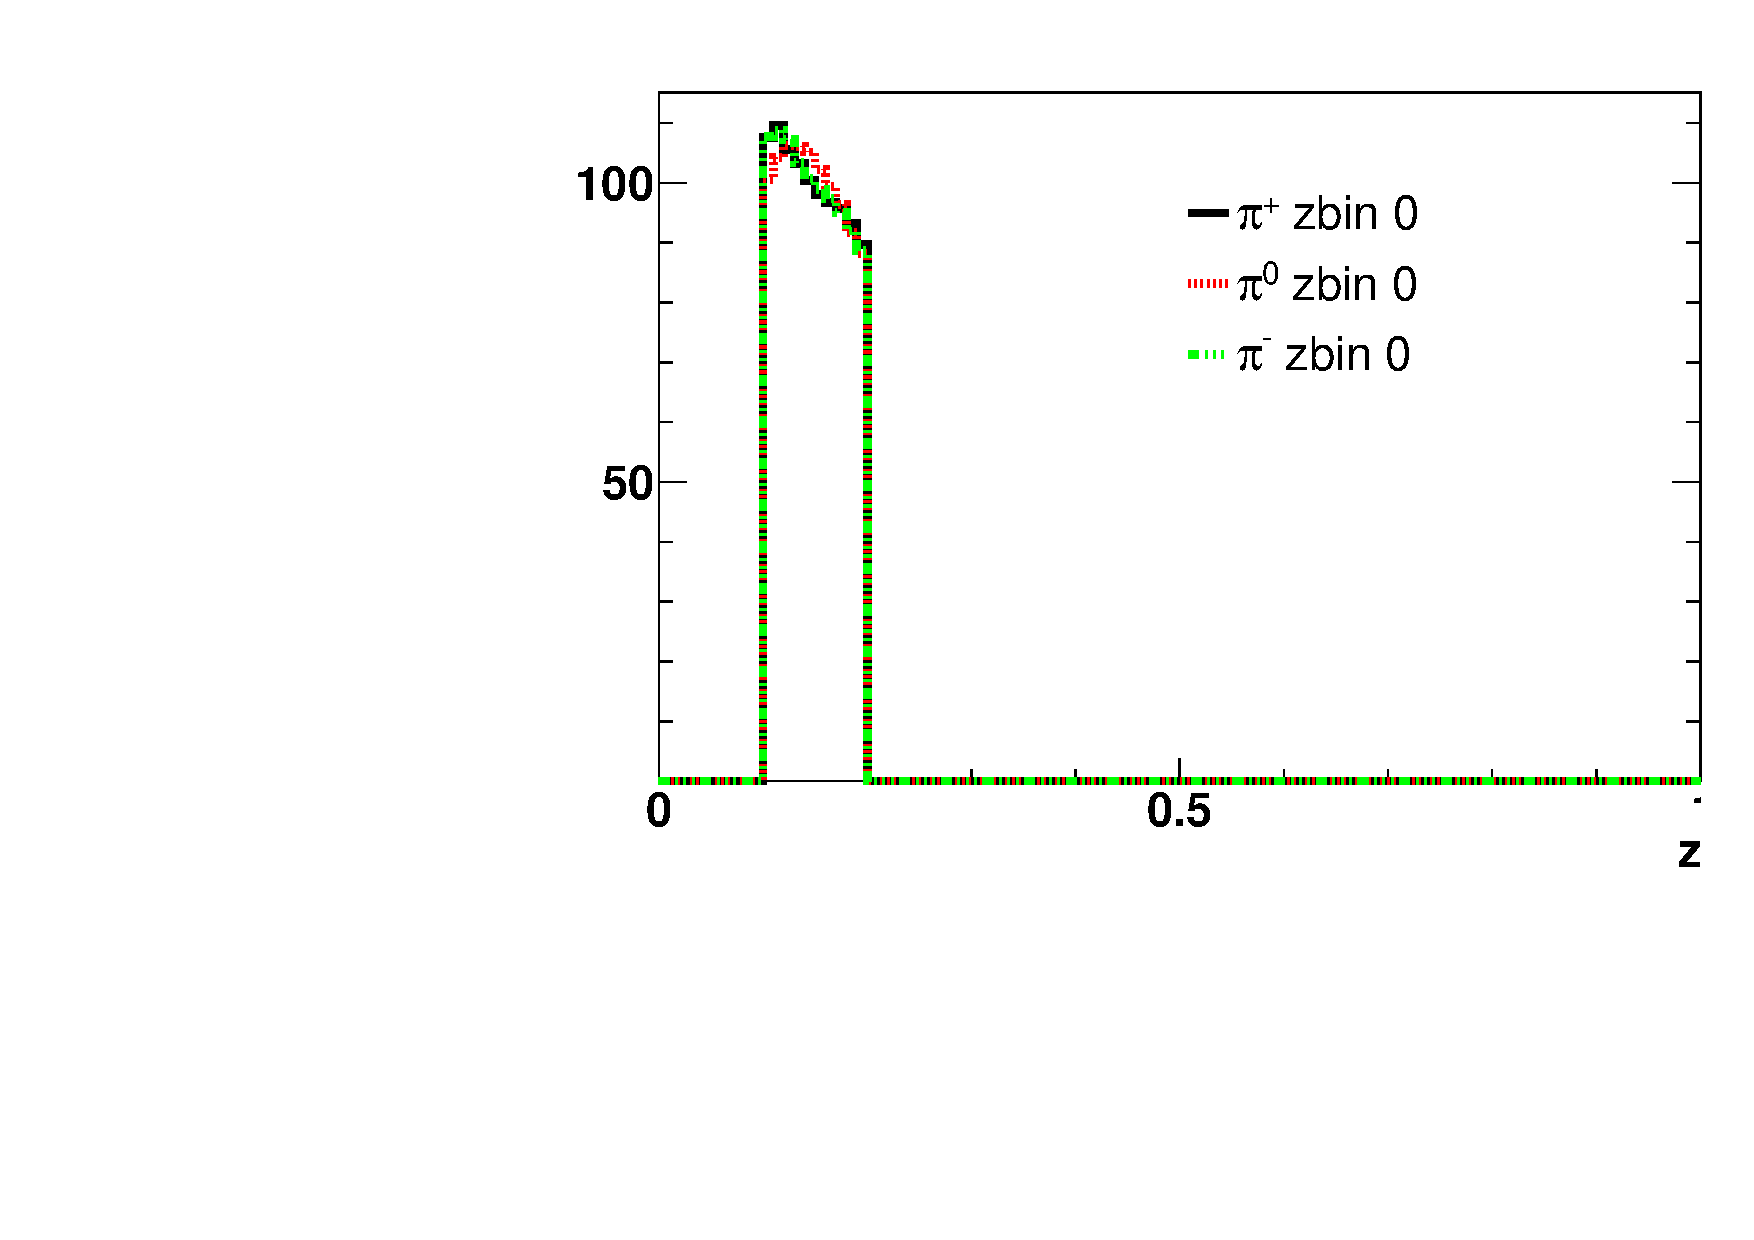
\includegraphics[width=.27\textwidth,natwidth=250,natheight=100]{figure_fiducial/had0.3/Z_distri_for_zbin_0_norm_had03.pdf}
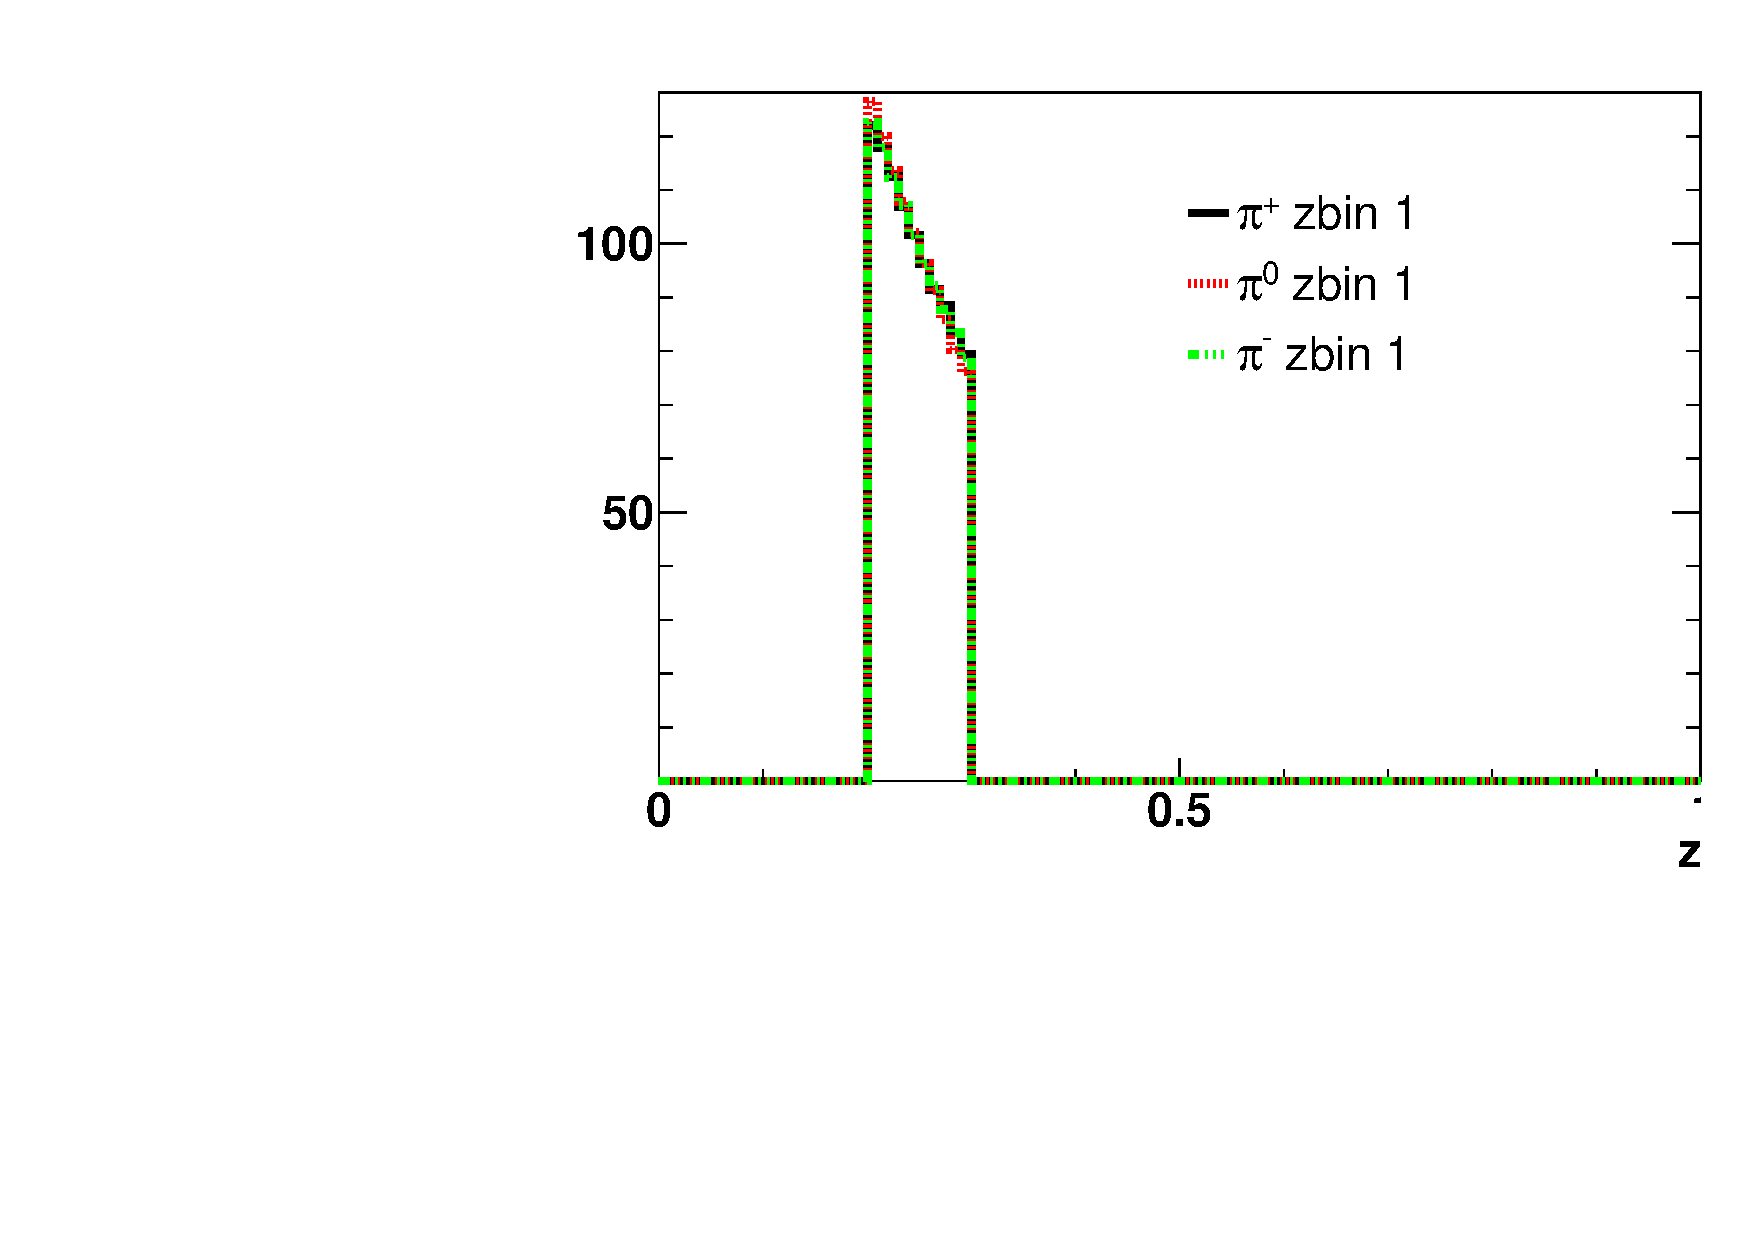
\includegraphics[width=.27\textwidth,natwidth=250,natheight=100]{figure_fiducial/had0.3/Z_distri_for_zbin_1_norm_had03.pdf}
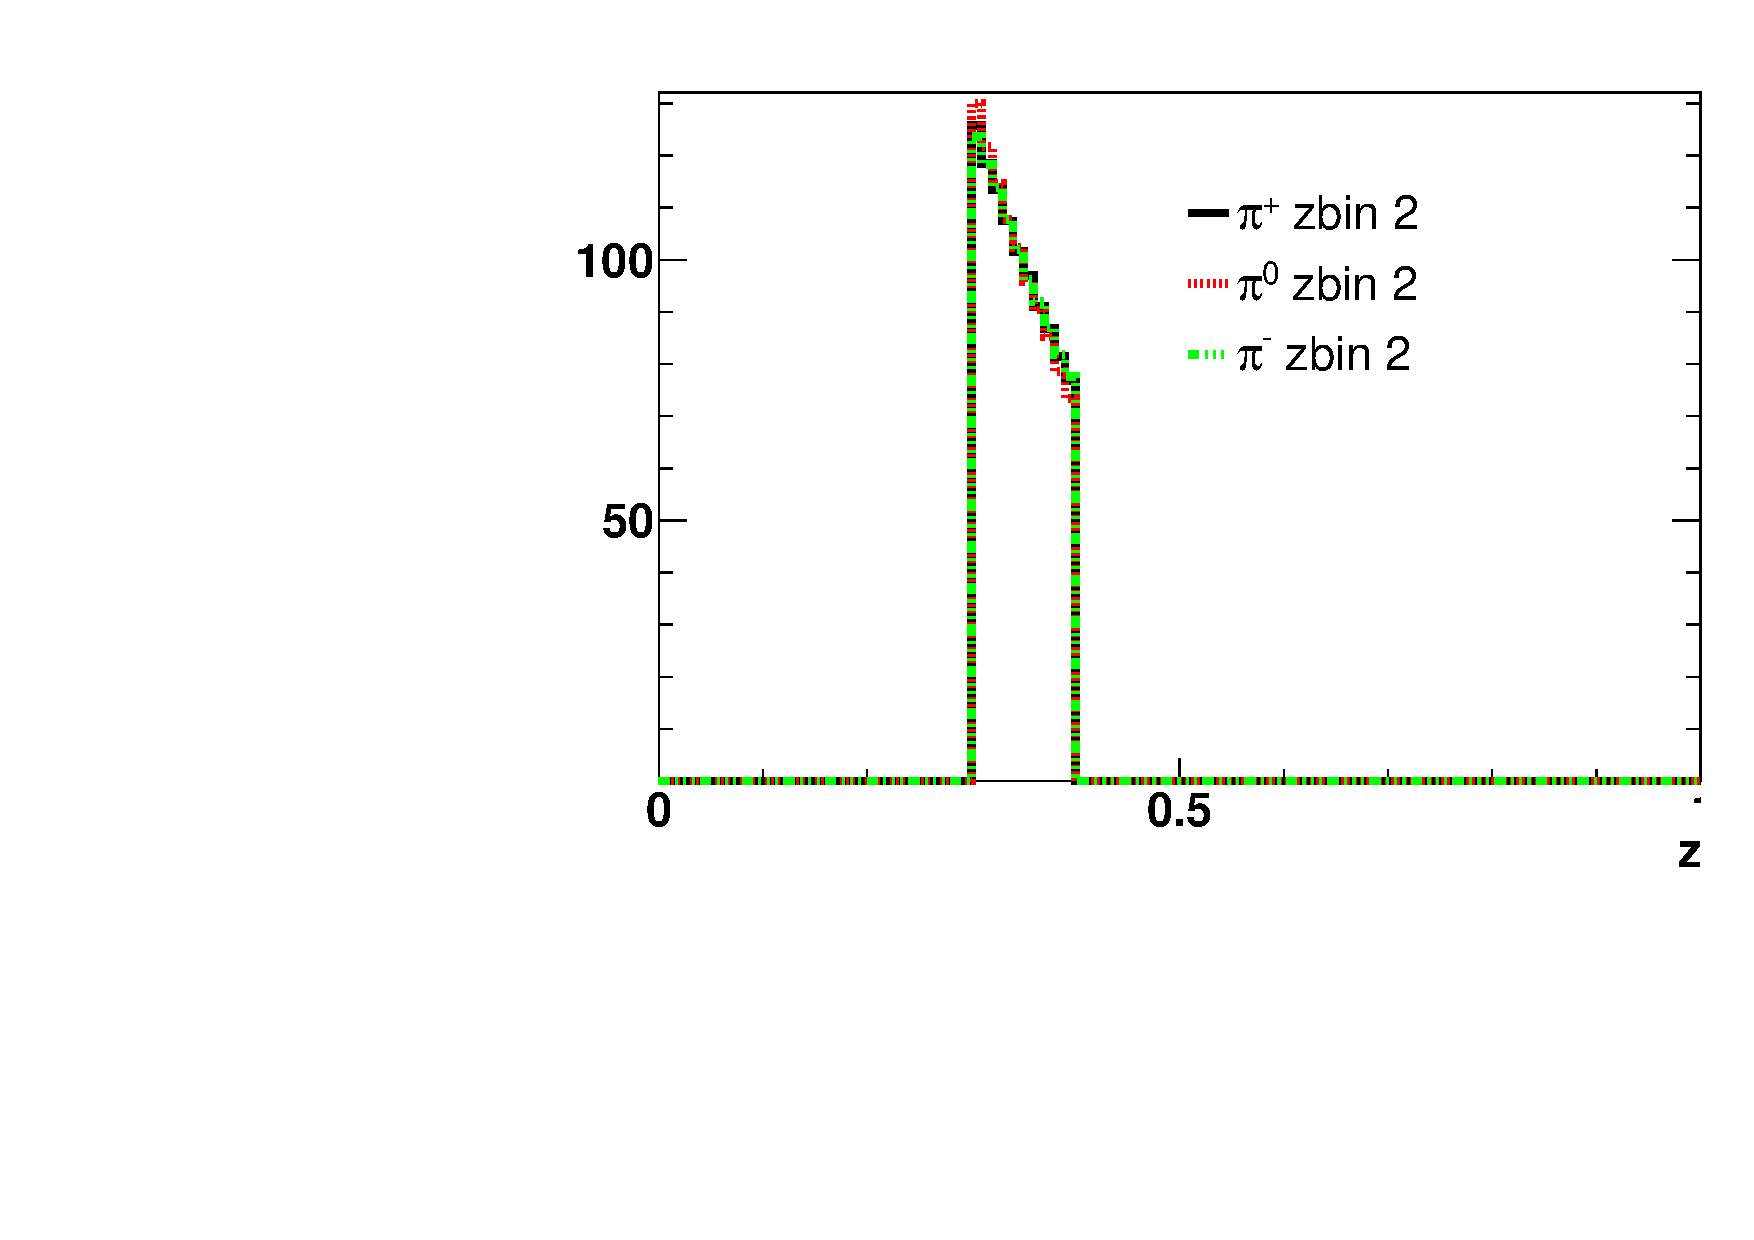
\includegraphics[width=.27\textwidth,natwidth=250,natheight=100]{figure_fiducial/had0.3/Z_distri_for_zbin_2_norm_had03.pdf}\hfill
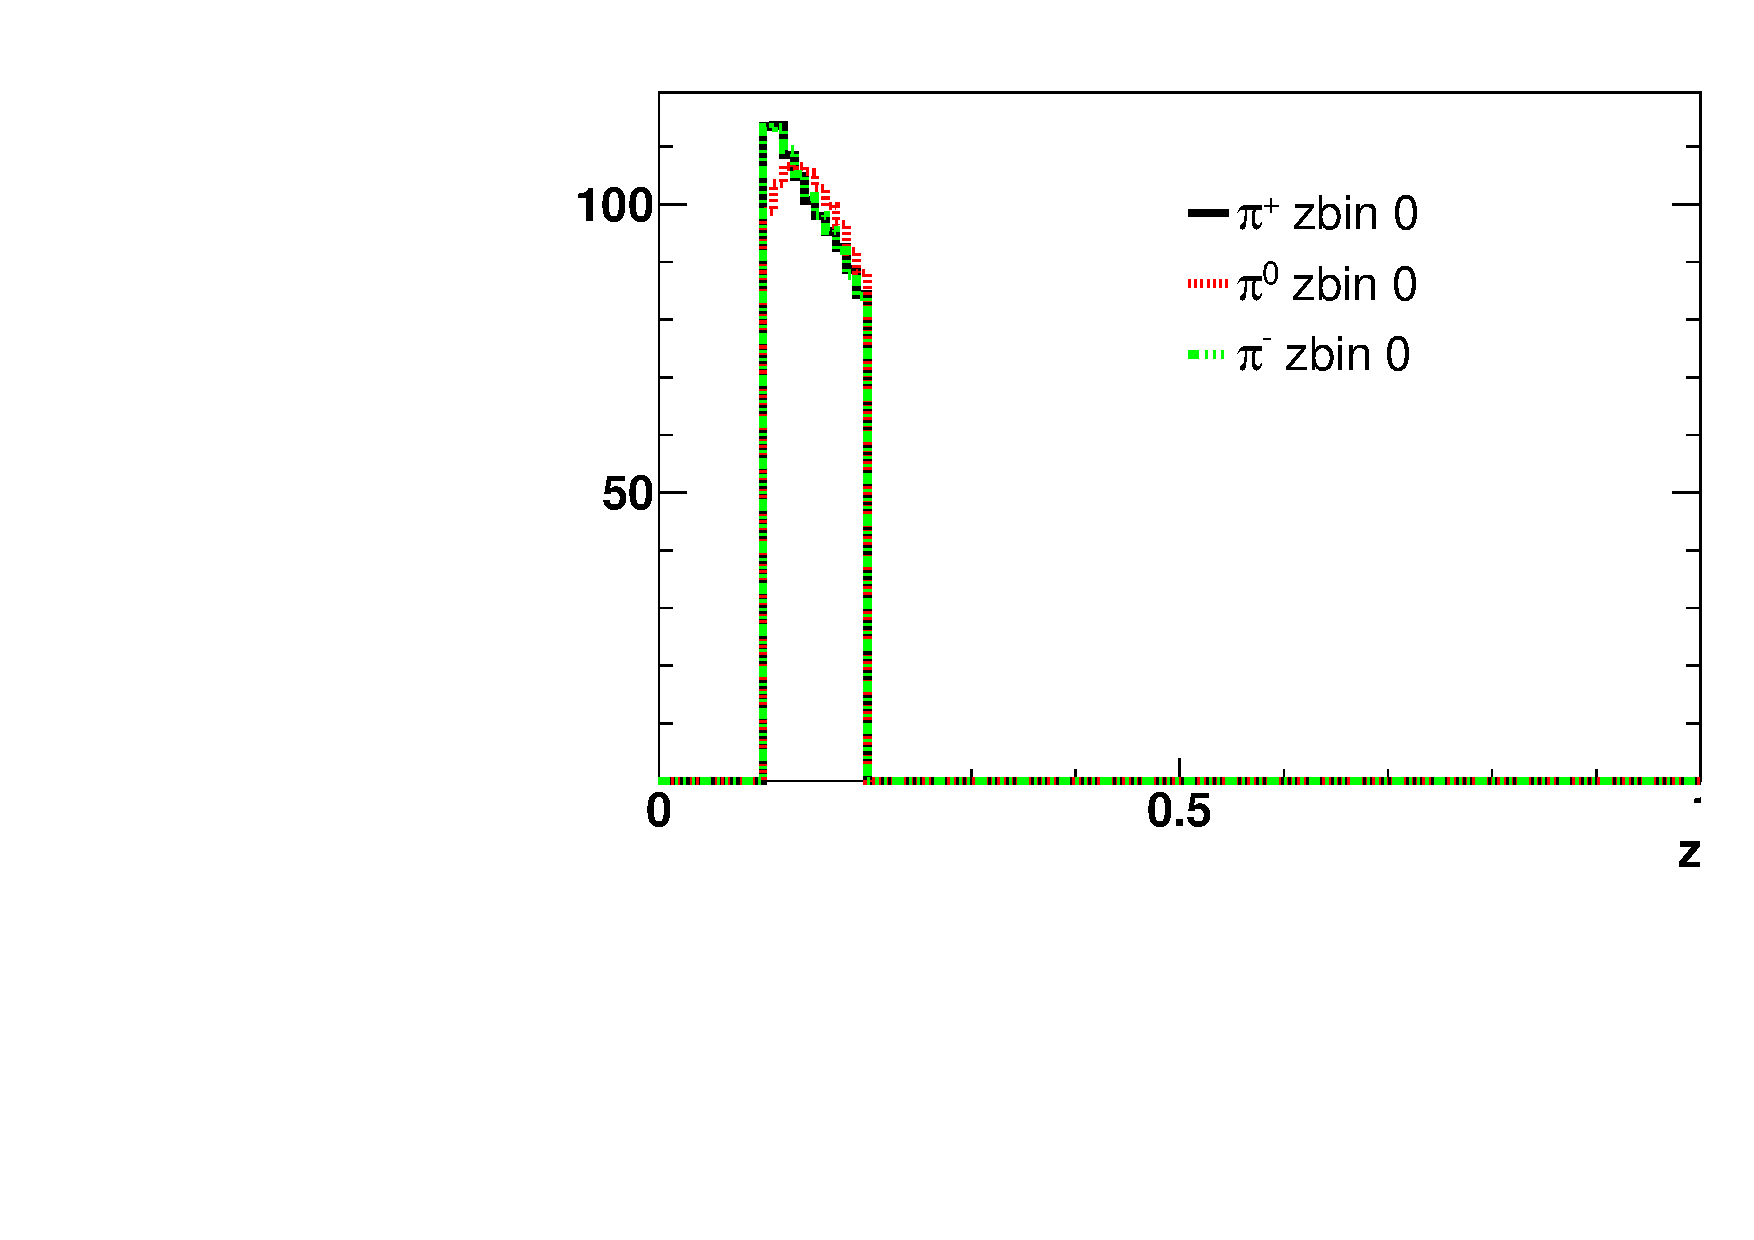
\includegraphics[width=.27\textwidth,natwidth=250,natheight=100]{figure_fiducial/had0.4/Z_distri_for_zbin_0_norm_had04.pdf}
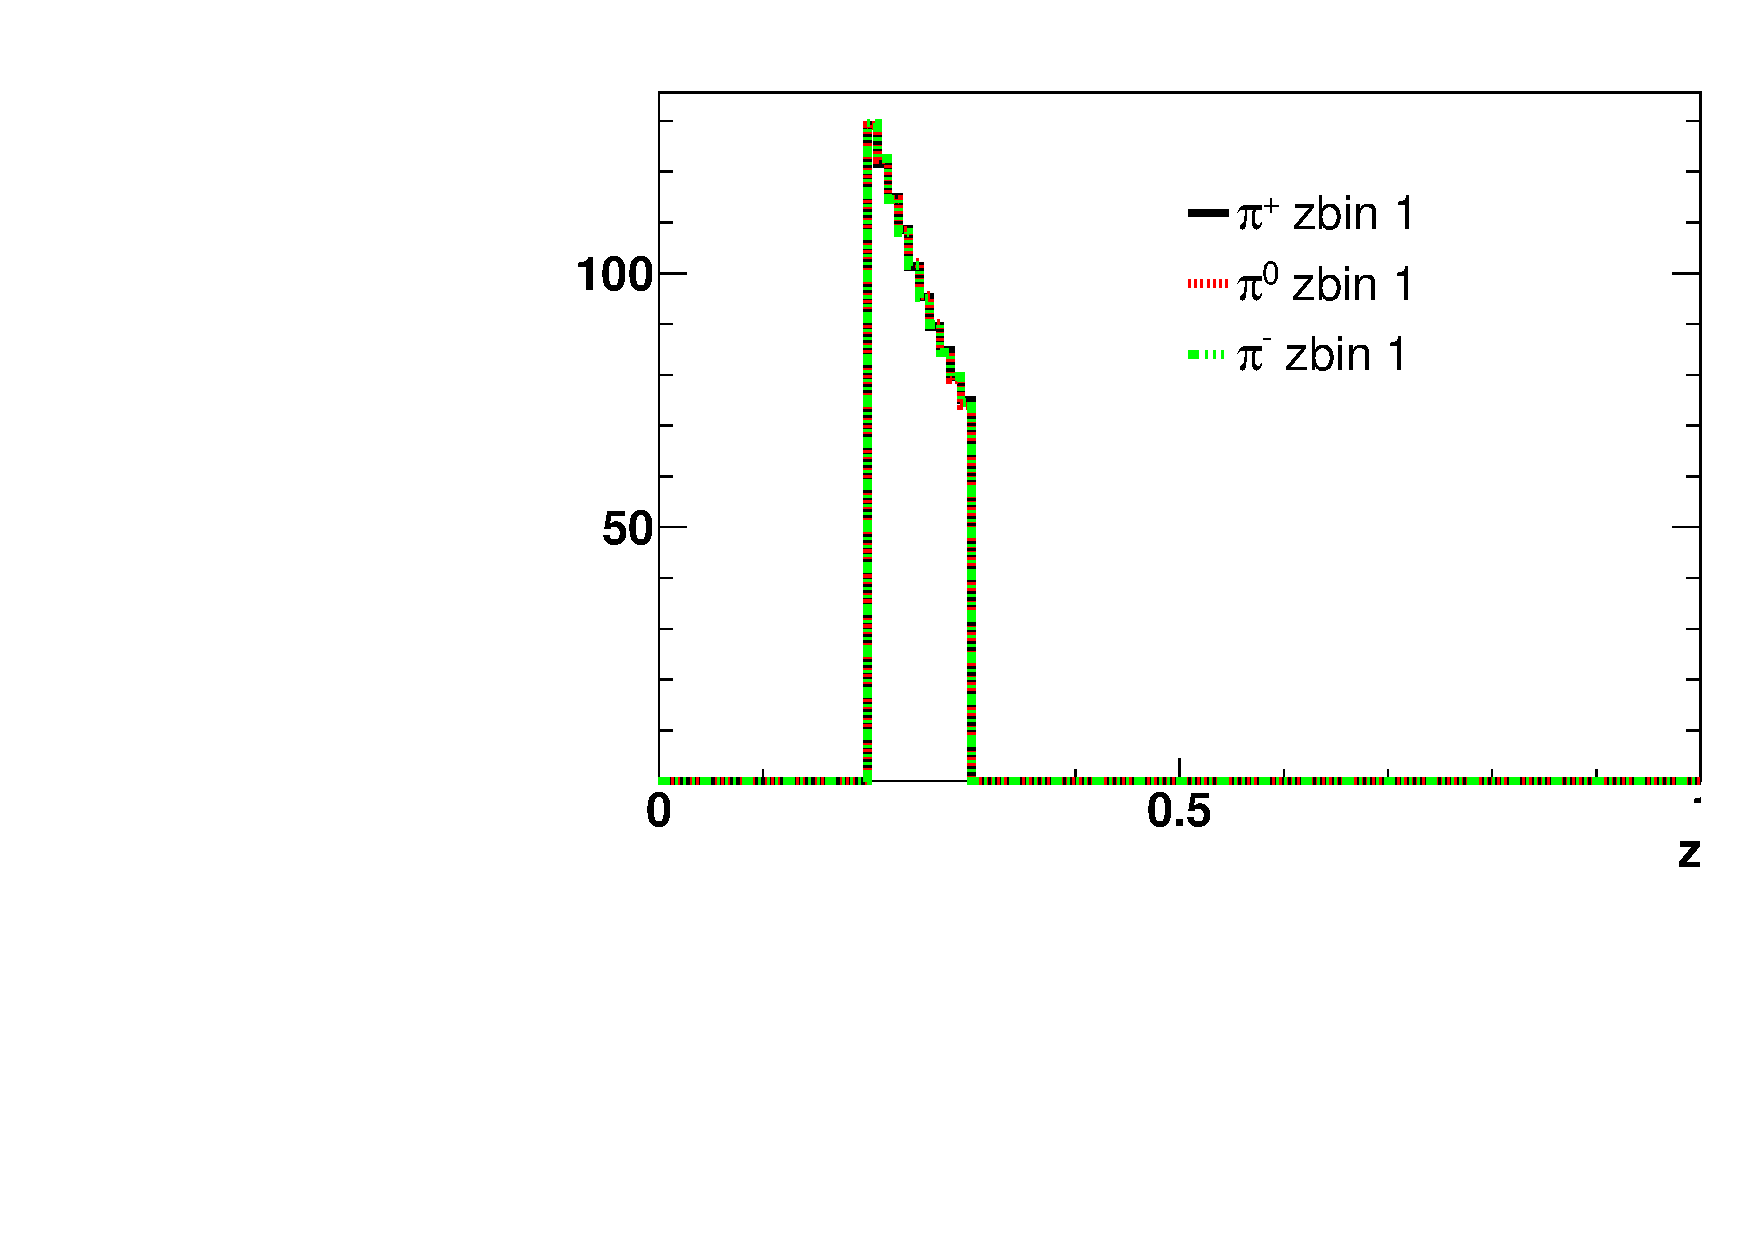
\includegraphics[width=.27\textwidth,natwidth=250,natheight=100]{figure_fiducial/had0.4/Z_distri_for_zbin_1_norm_had04.pdf}
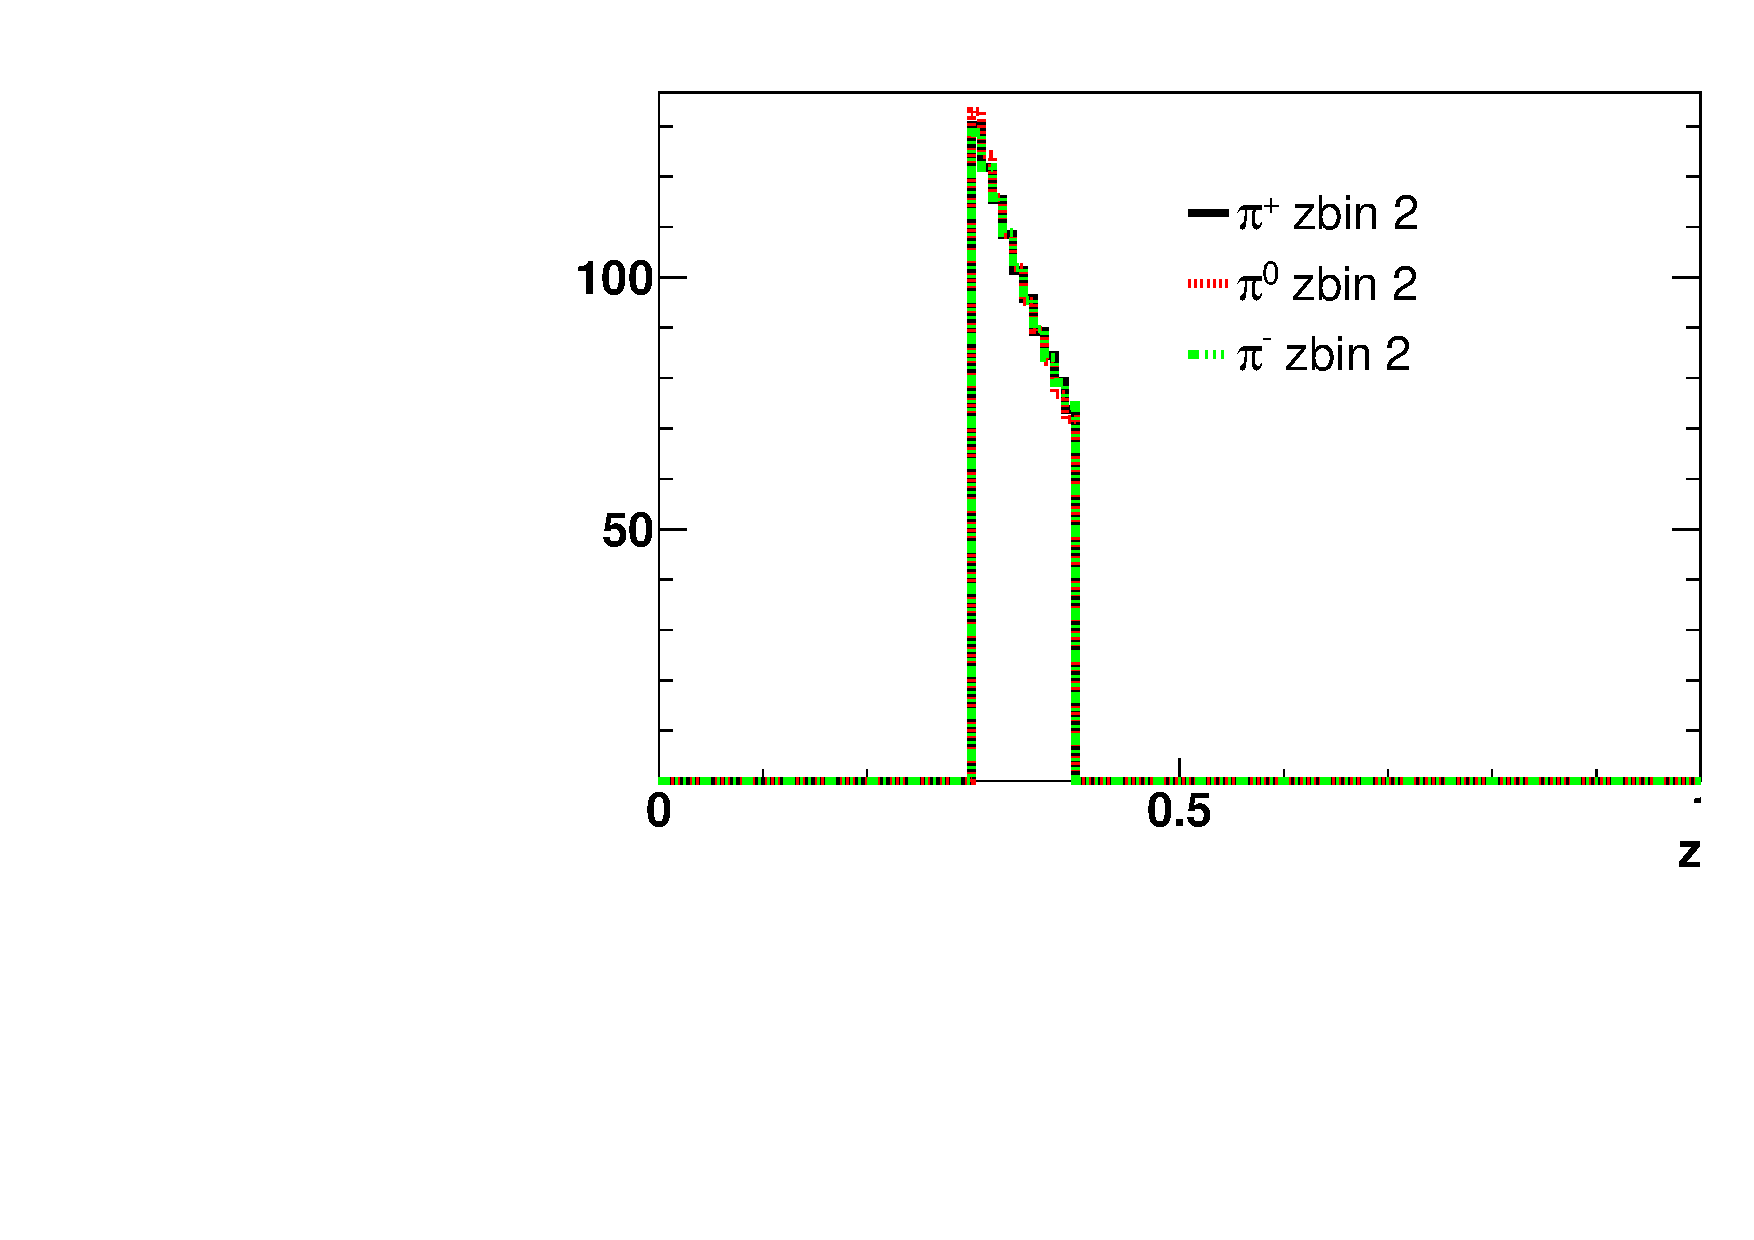
\includegraphics[width=.27\textwidth,natwidth=250,natheight=100]{figure_fiducial/had0.4/Z_distri_for_zbin_2_norm_had04.pdf}\hfill
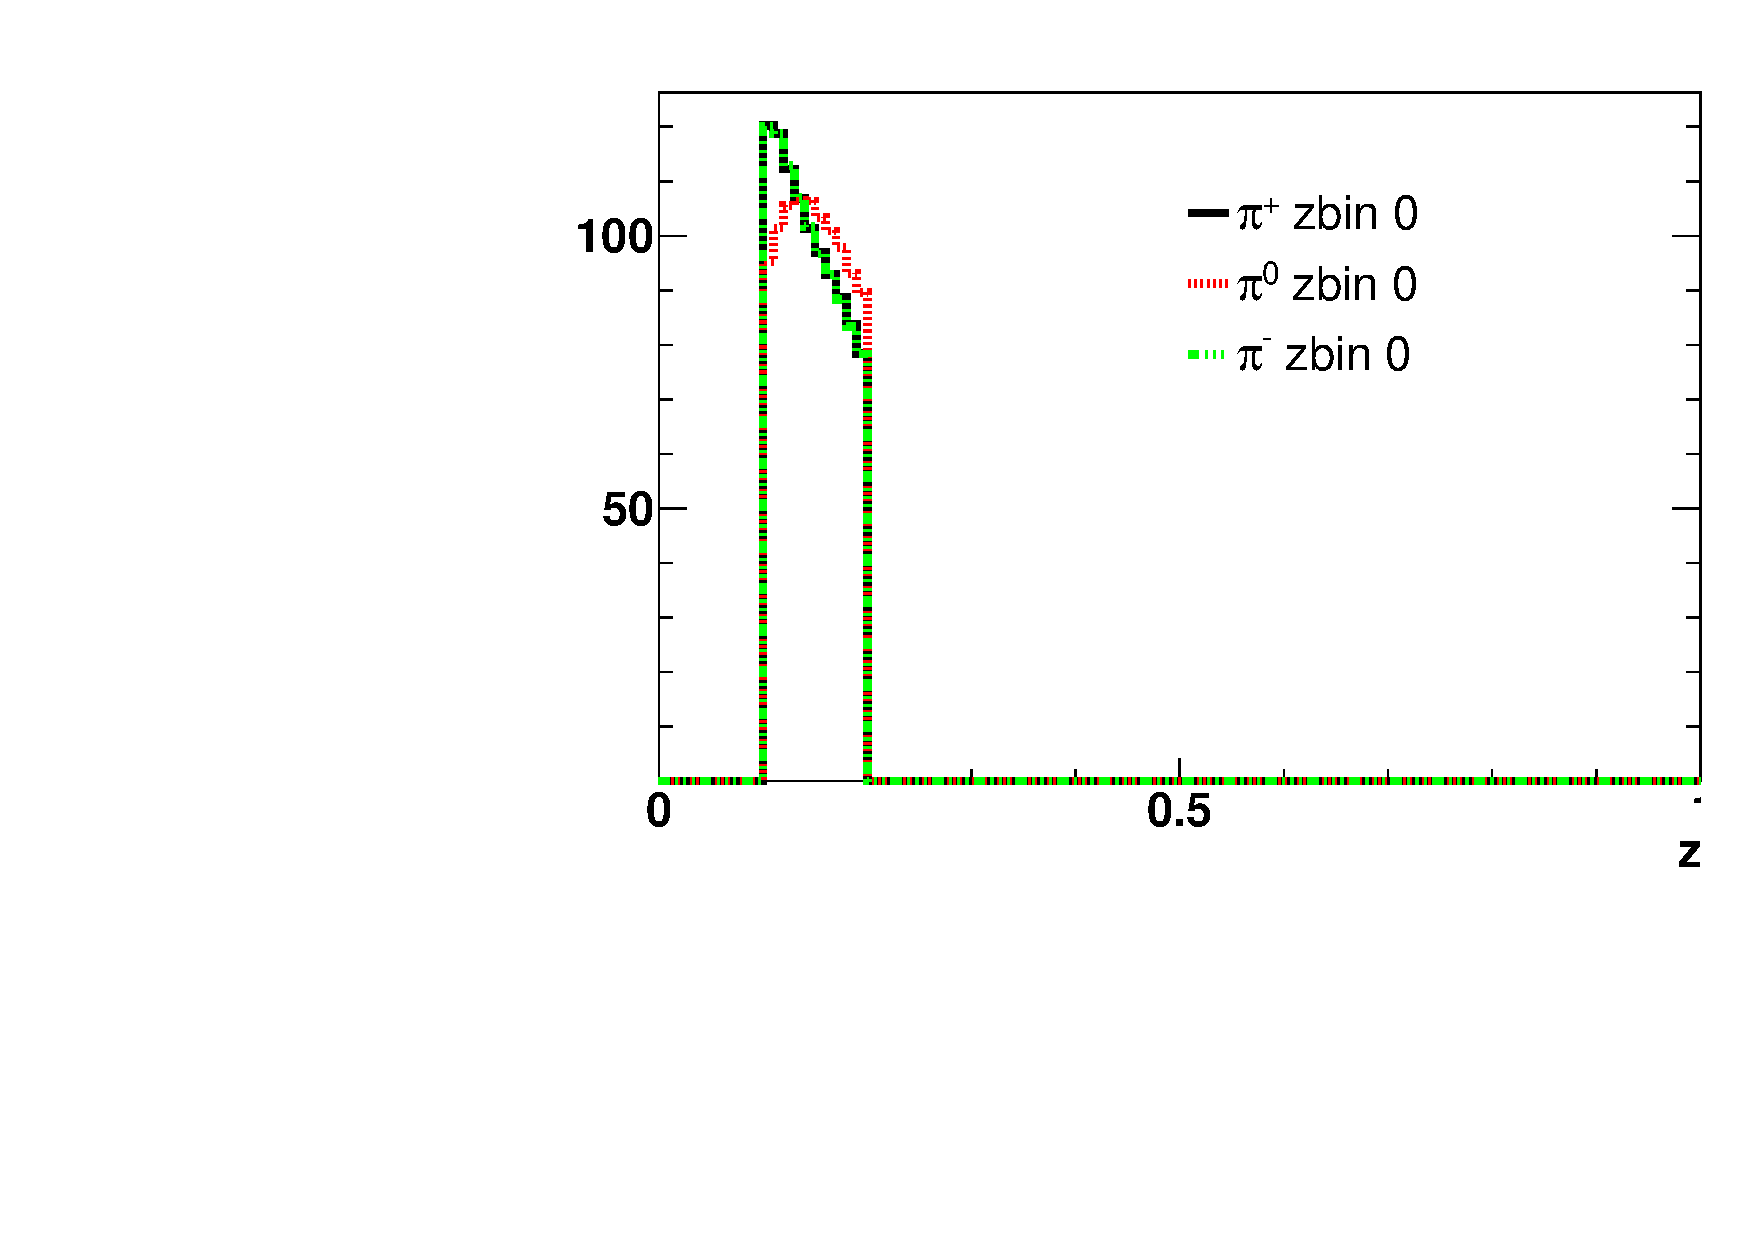
\includegraphics[width=.27\textwidth,natwidth=250,natheight=100]{figure_fiducial/had0.5/Z_distri_for_zbin_0_norm_had05.pdf}
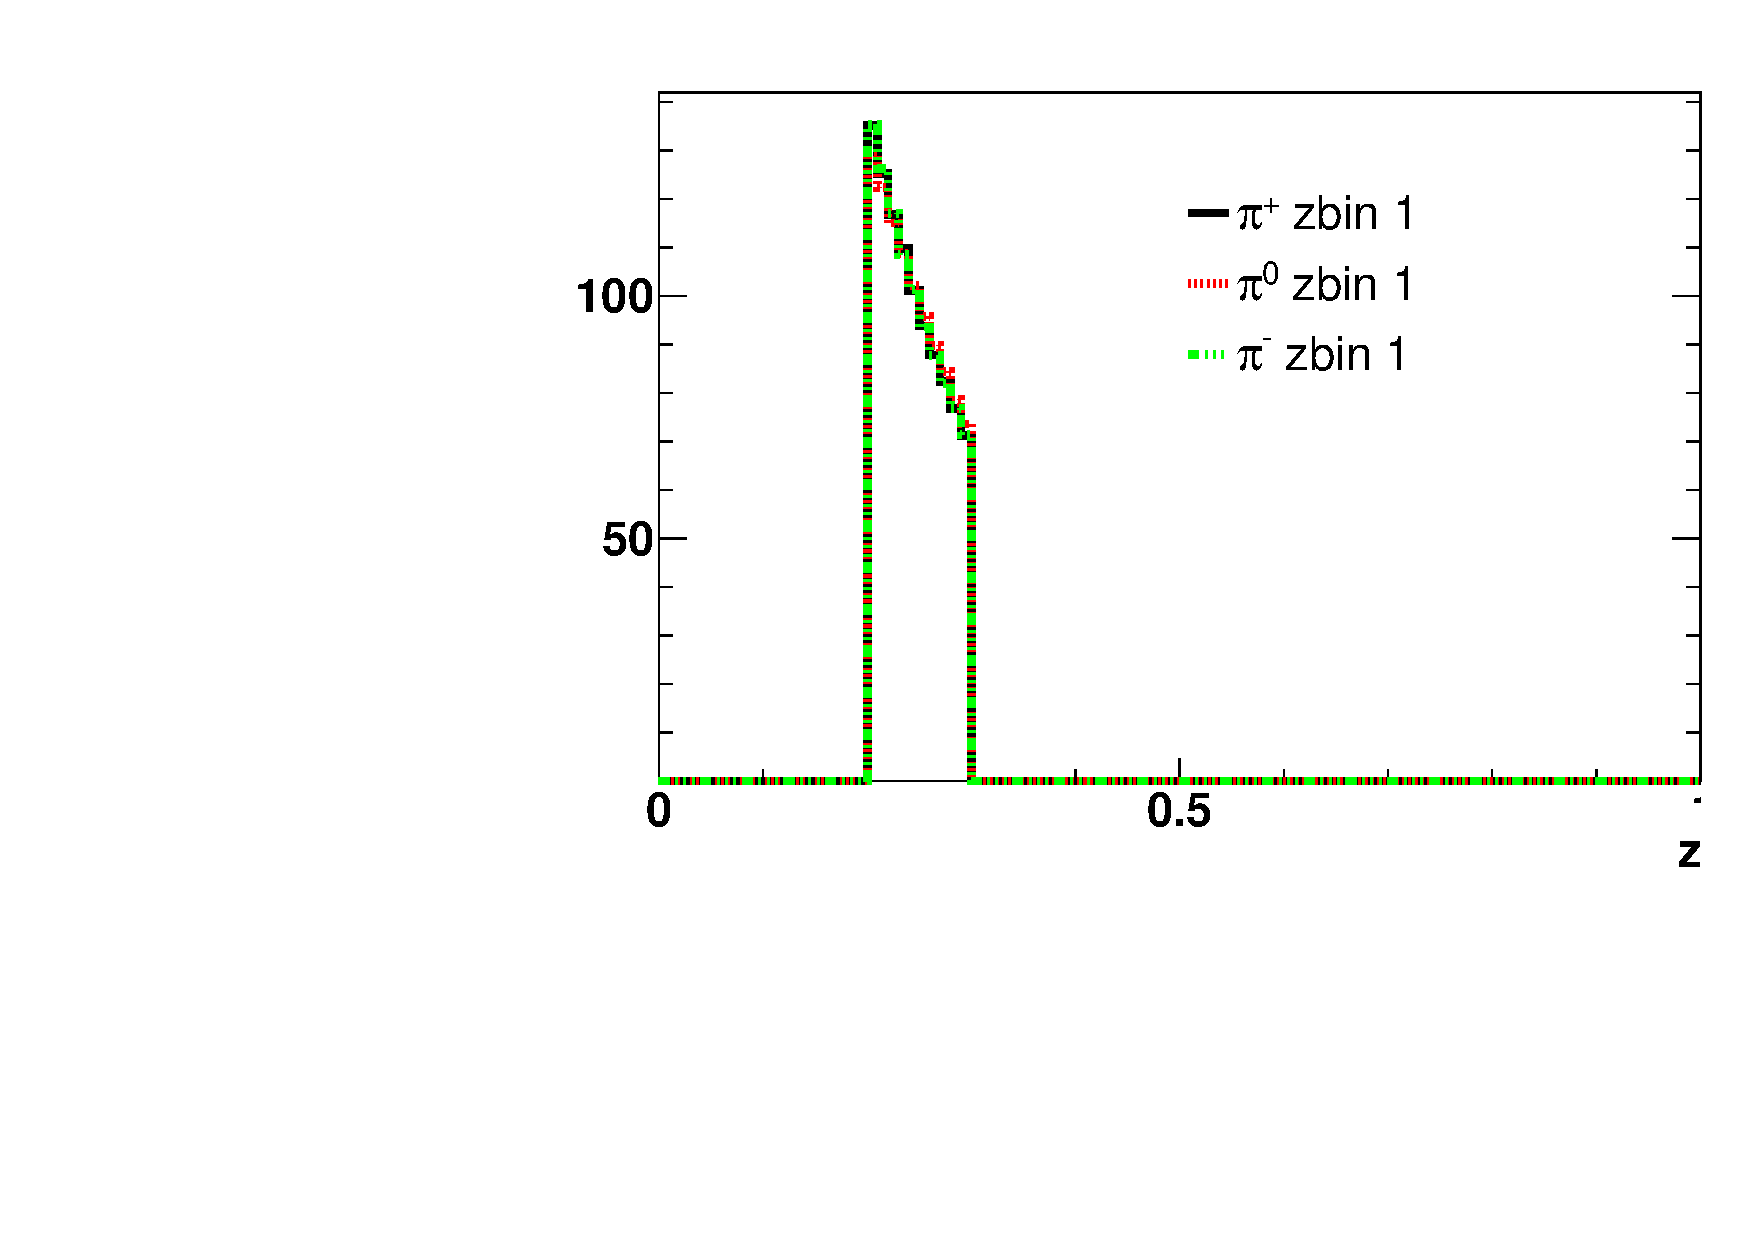
\includegraphics[width=.27\textwidth,natwidth=250,natheight=100]{figure_fiducial/had0.5/Z_distri_for_zbin_1_norm_had05.pdf}
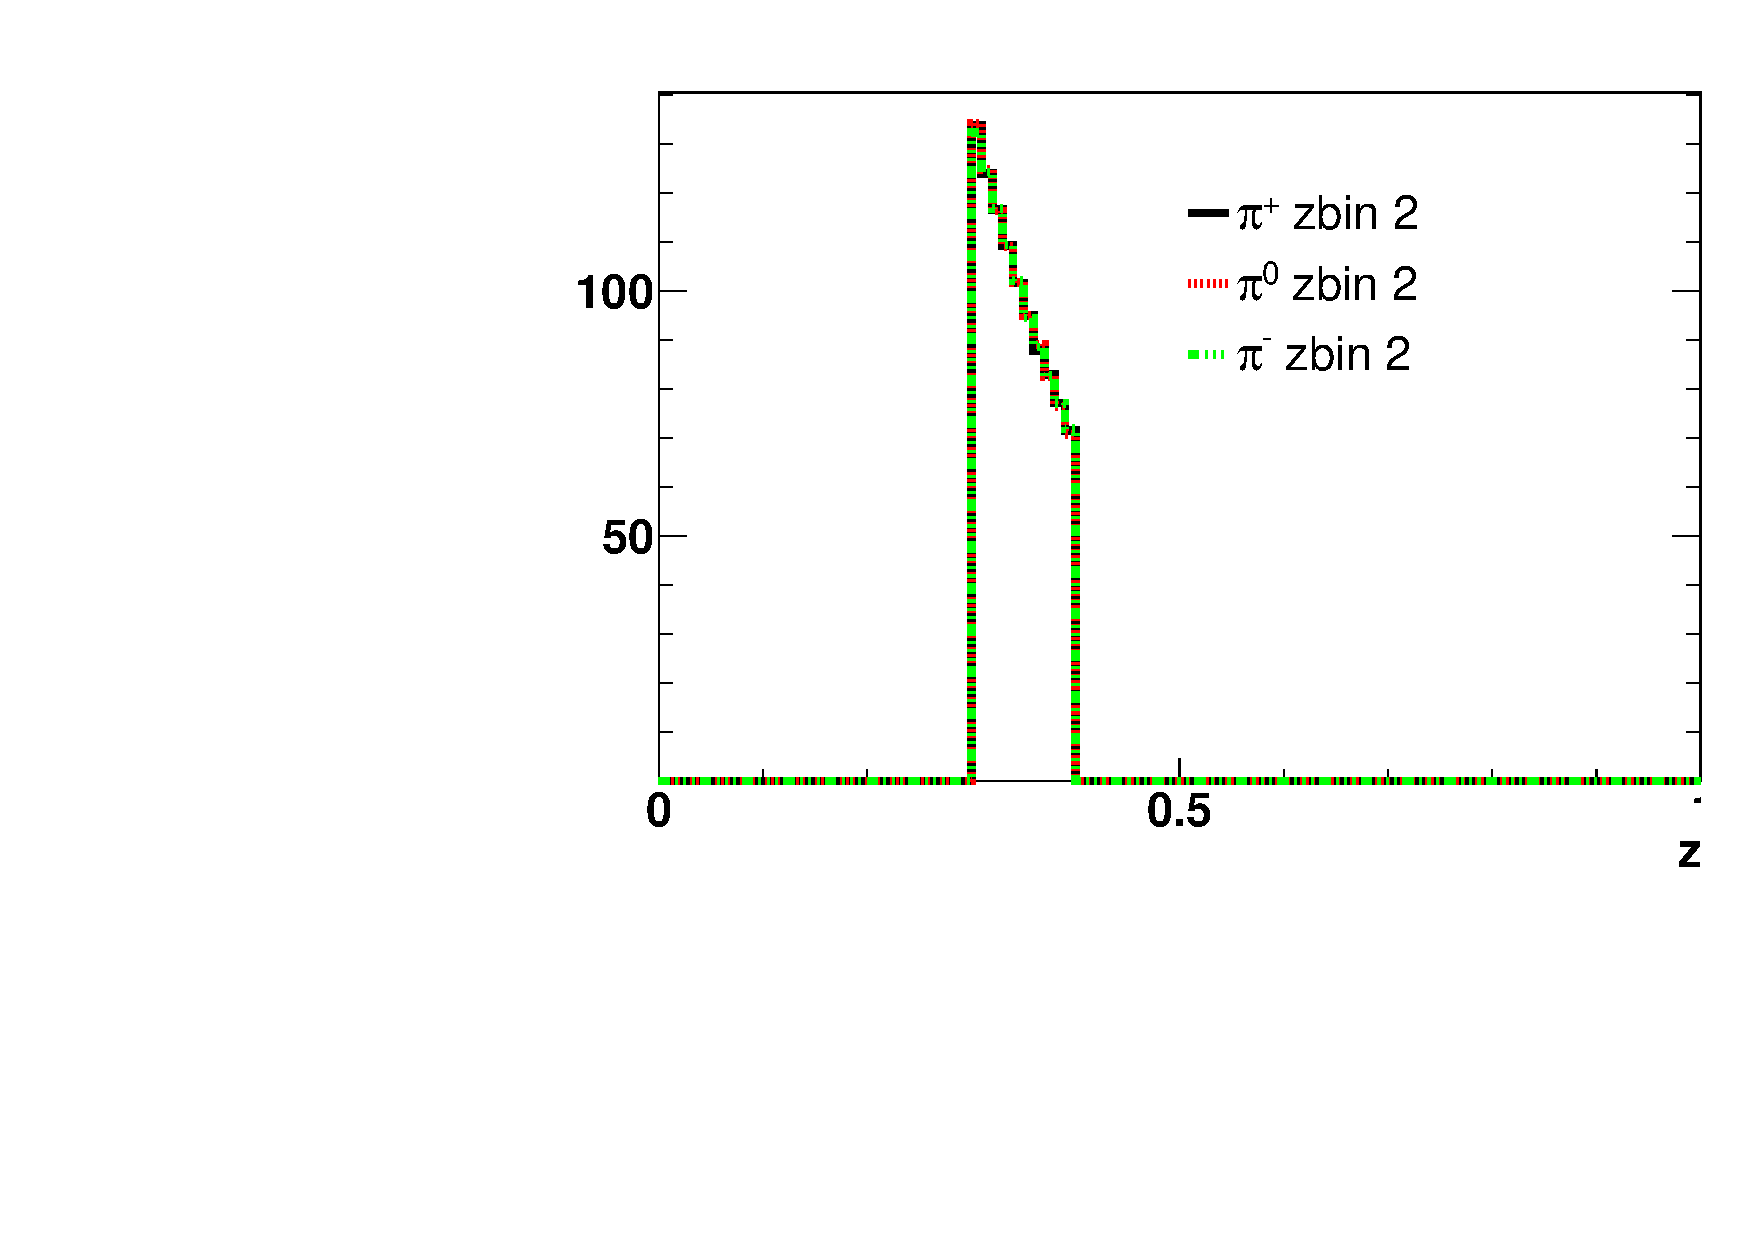
\includegraphics[width=.27\textwidth,natwidth=250,natheight=100]{figure_fiducial/had0.5/Z_distri_for_zbin_2_norm_had05.pdf}\hfill
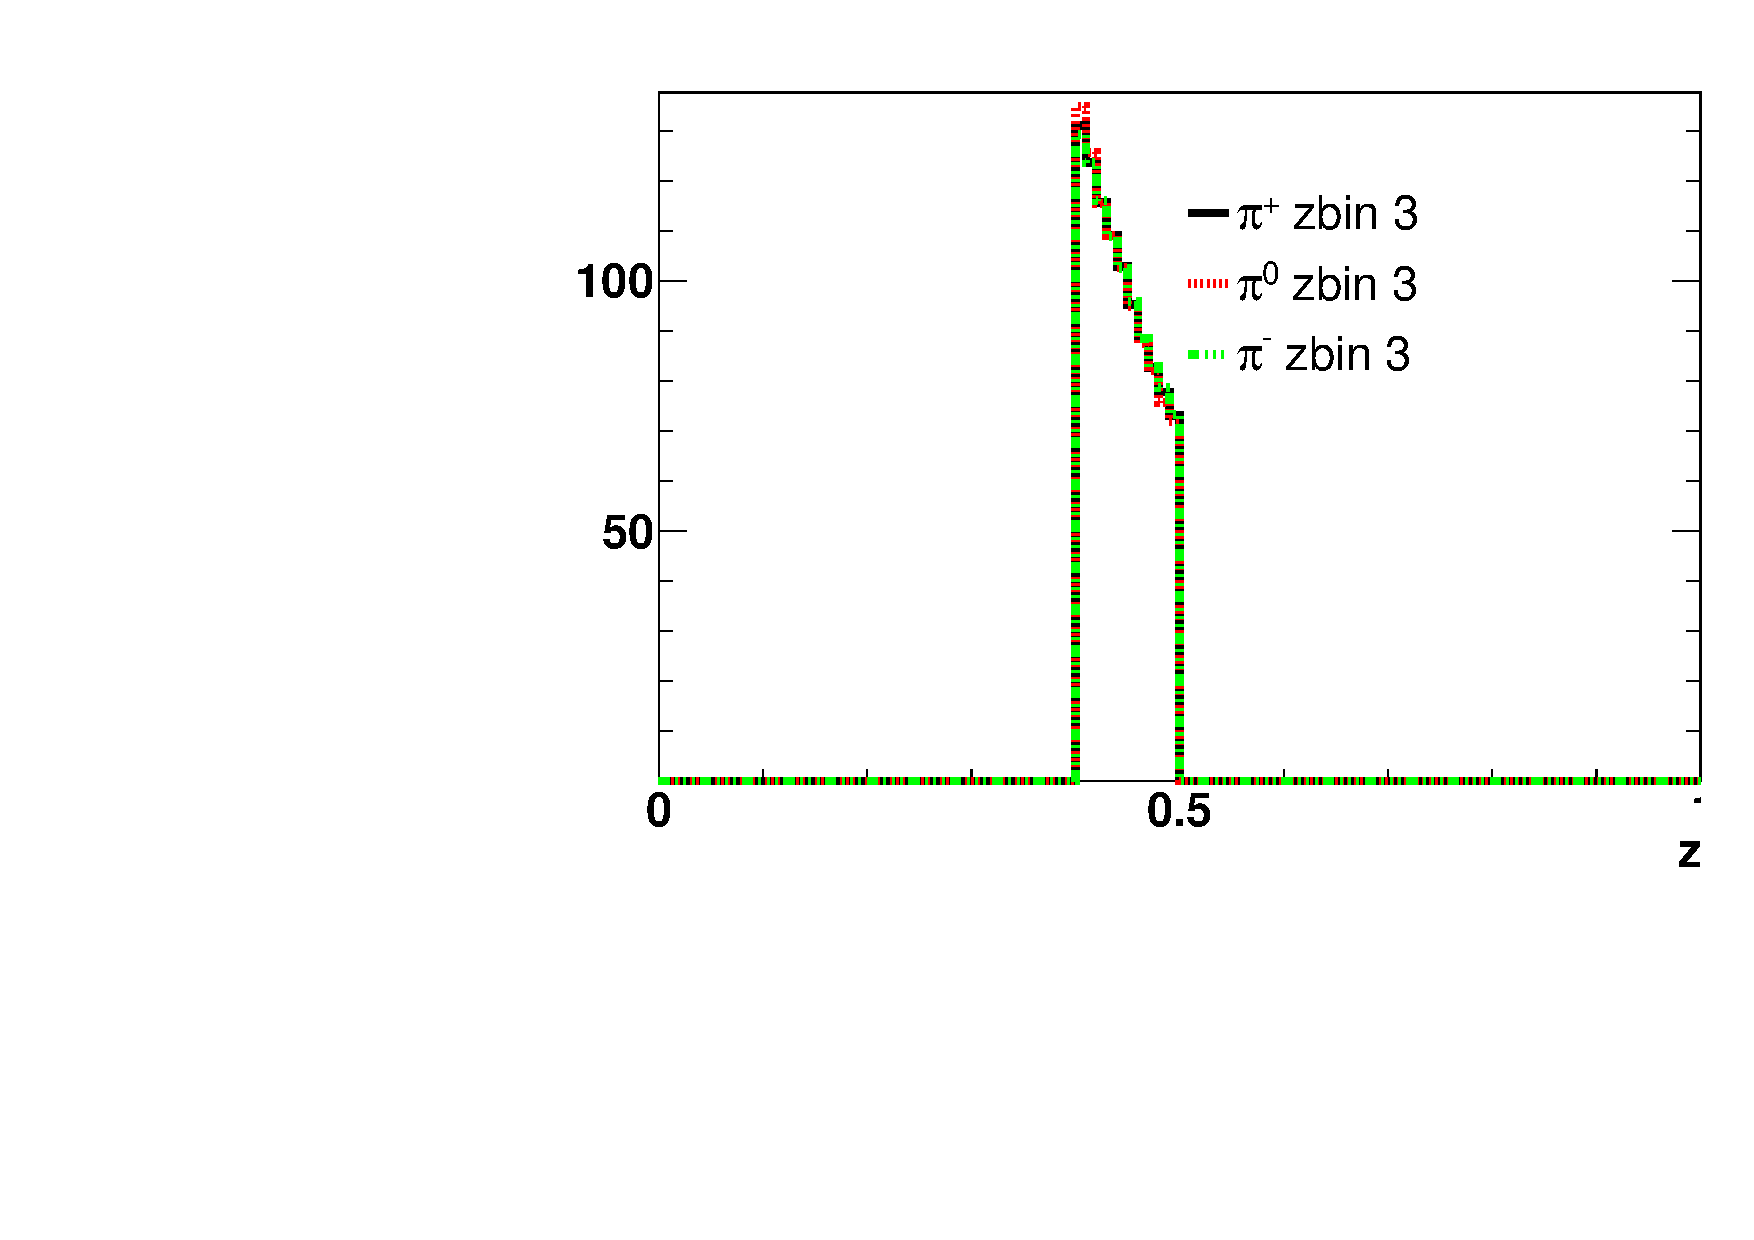
\includegraphics[width=.27\textwidth,natwidth=250,natheight=100]{figure_fiducial/had0.3/Z_distri_for_zbin_3_norm_had03.pdf}
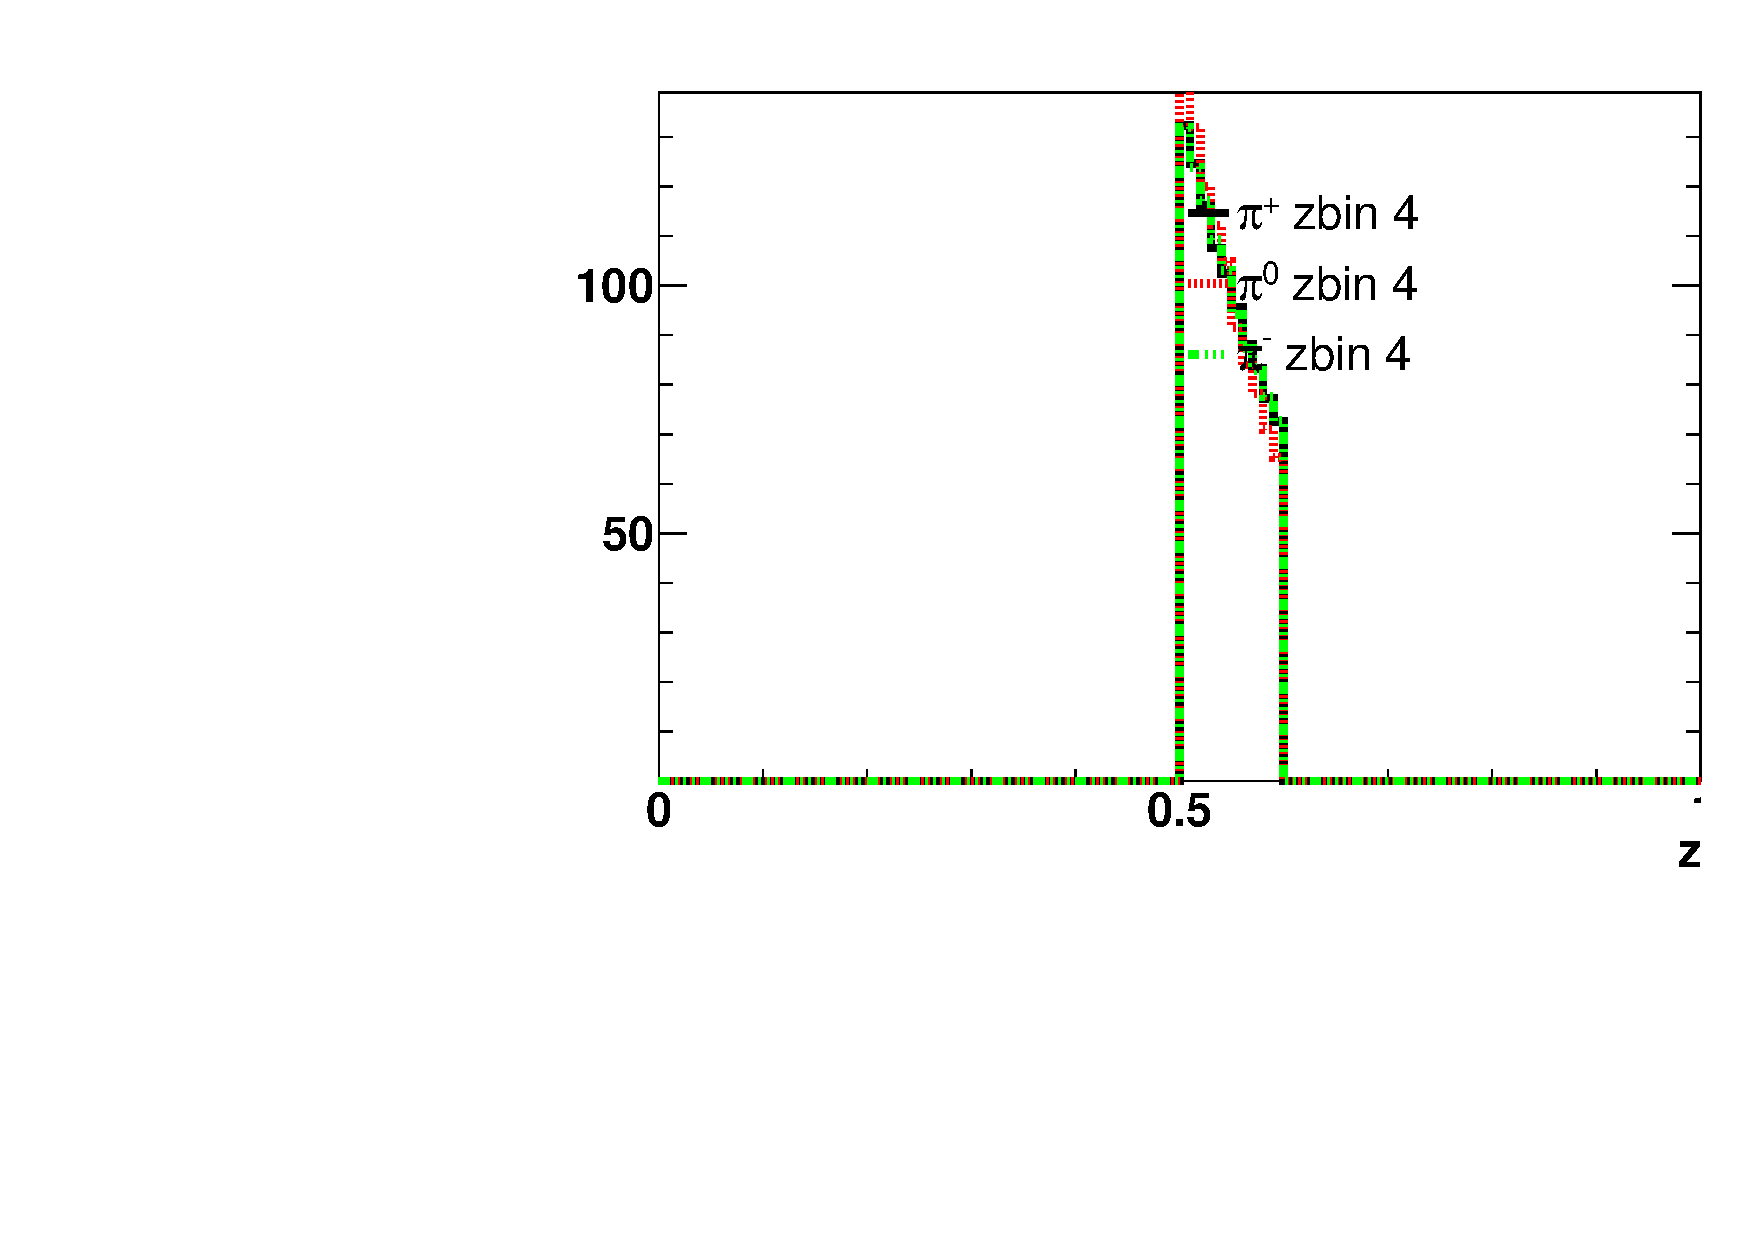
\includegraphics[width=.27\textwidth,natwidth=250,natheight=100]{figure_fiducial/had0.3/Z_distri_for_zbin_4_norm_had03.pdf}
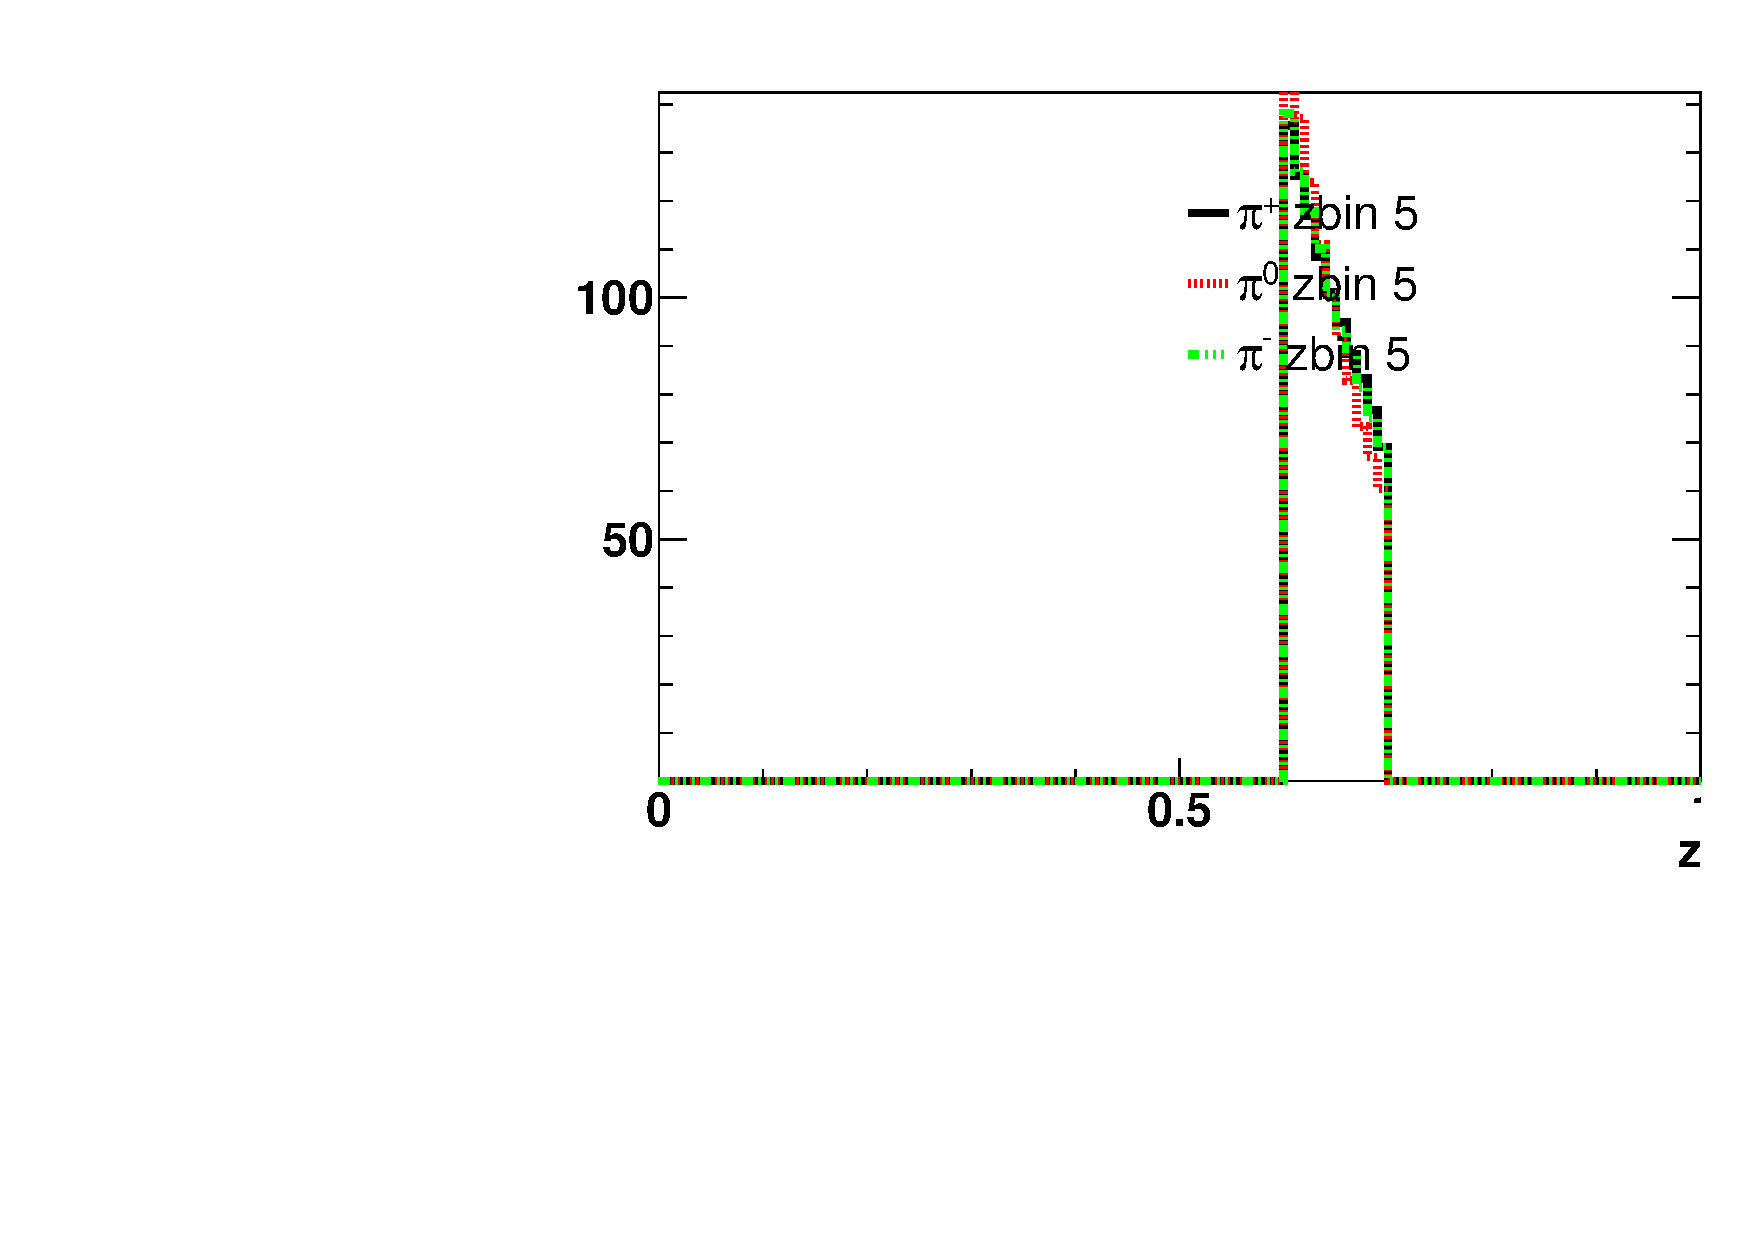
\includegraphics[width=.27\textwidth,natwidth=250,natheight=100]{figure_fiducial/had0.3/Z_distri_for_zbin_5_norm_had03.pdf}\hfill
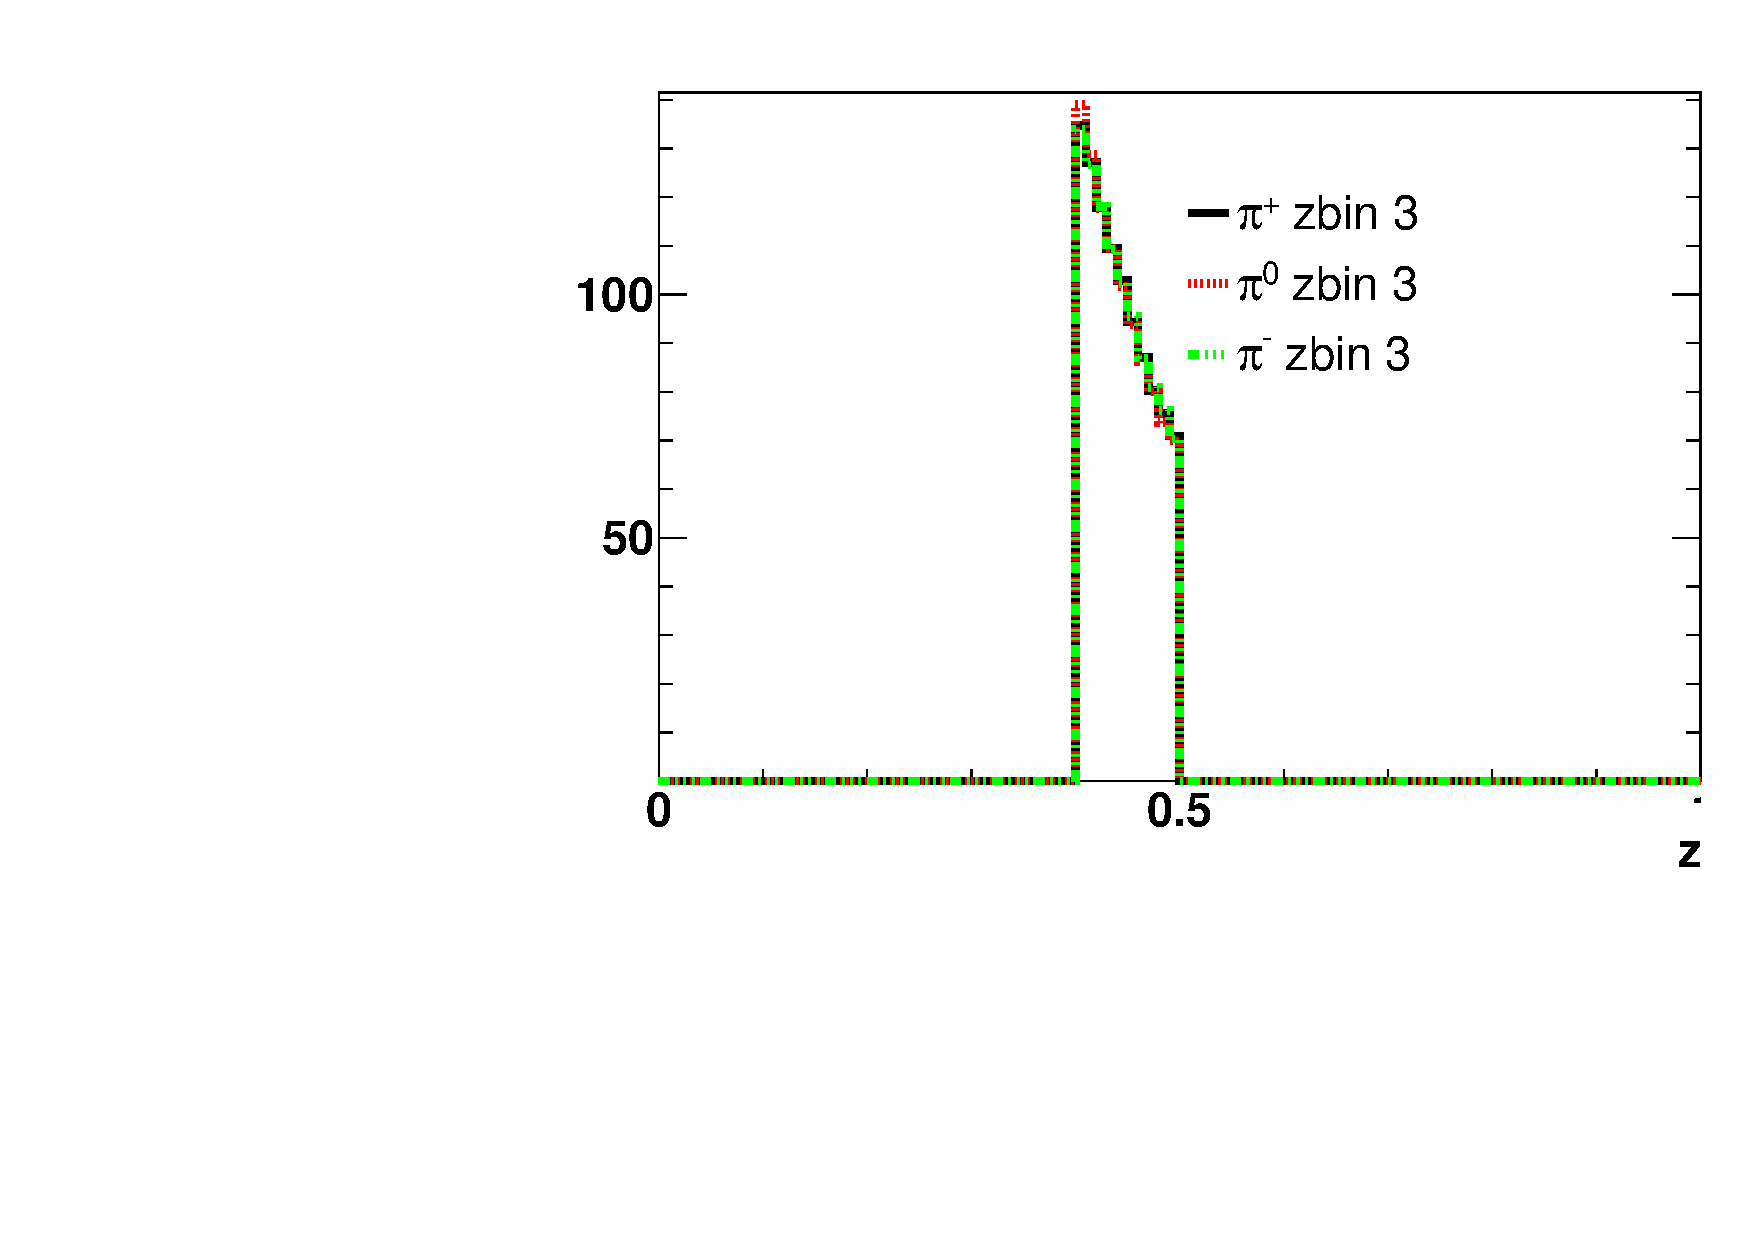
\includegraphics[width=.27\textwidth,natwidth=250,natheight=100]{figure_fiducial/had0.4/Z_distri_for_zbin_3_norm_had04.pdf}
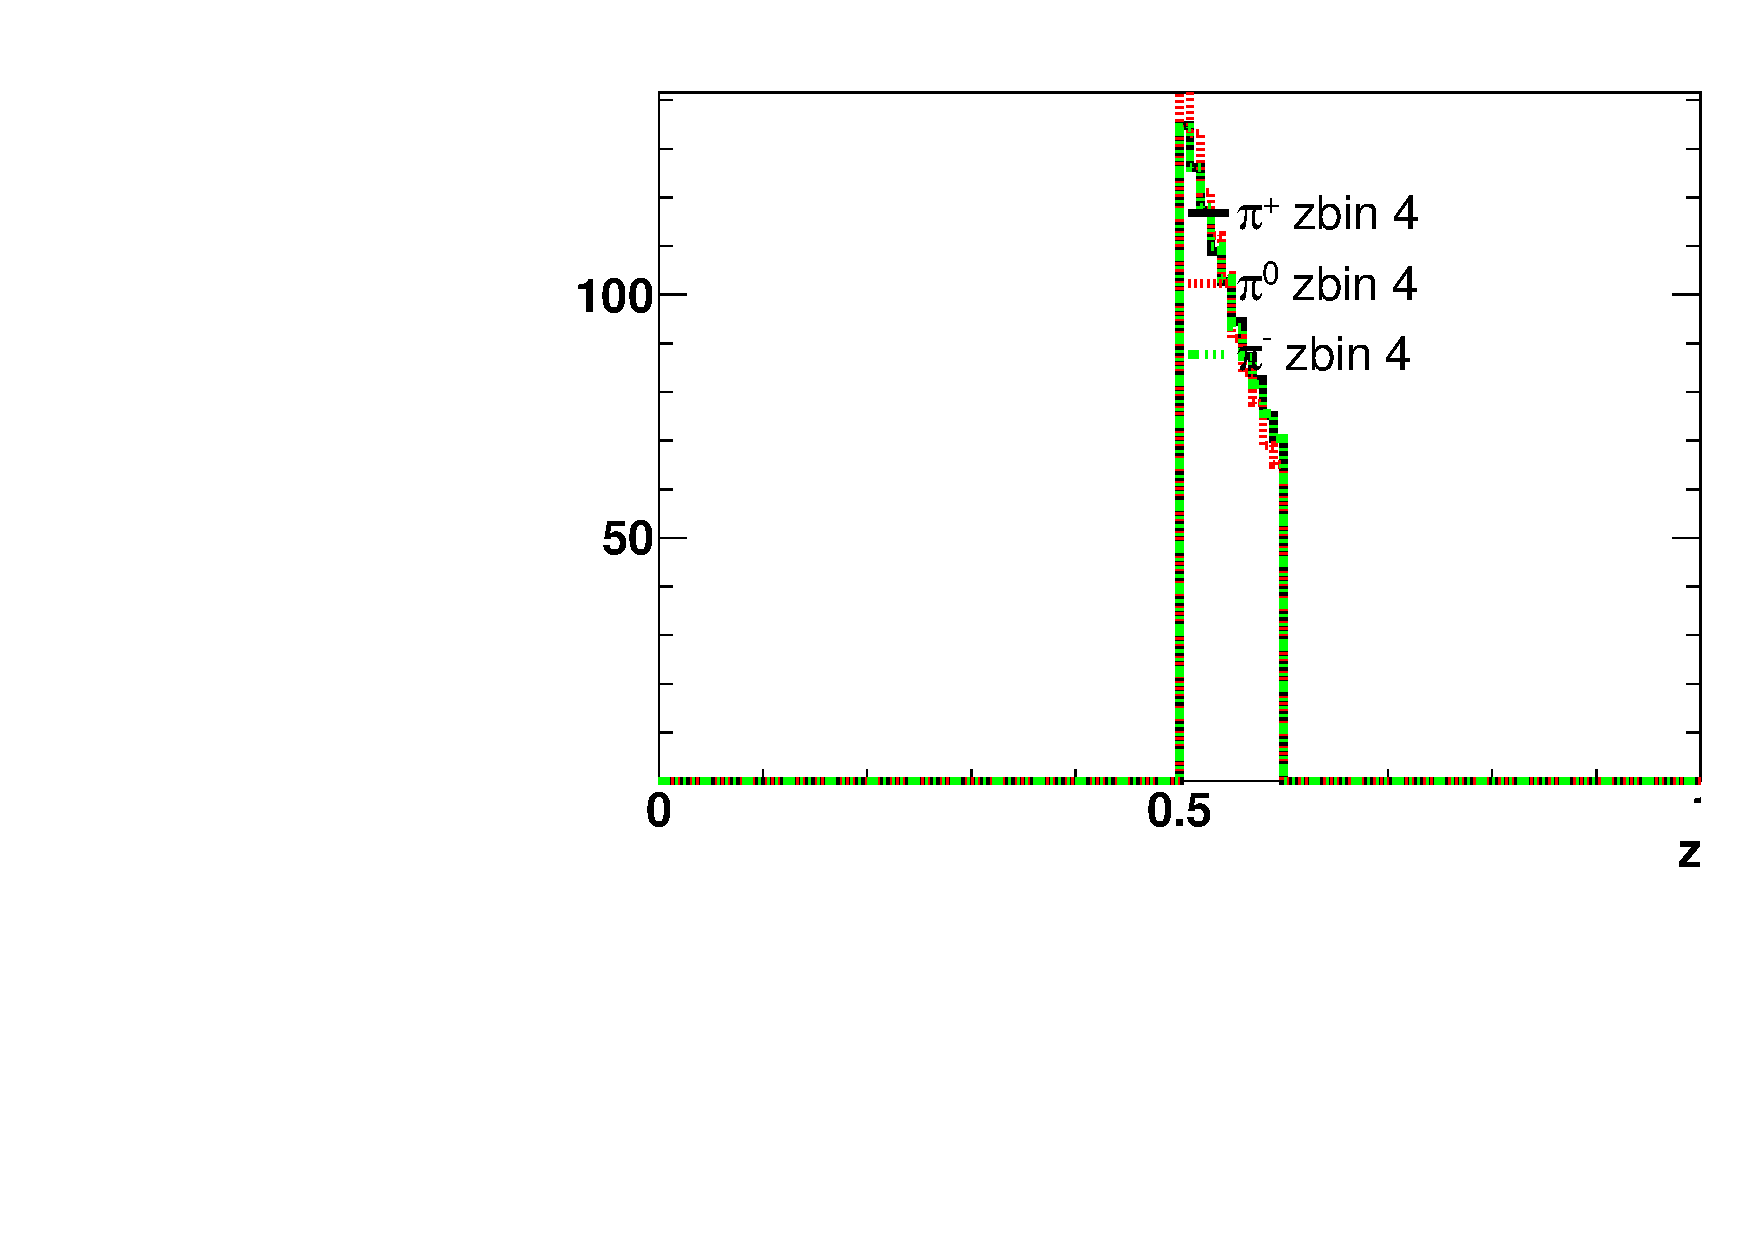
\includegraphics[width=.27\textwidth,natwidth=250,natheight=100]{figure_fiducial/had0.4/Z_distri_for_zbin_4_norm_had04.pdf}
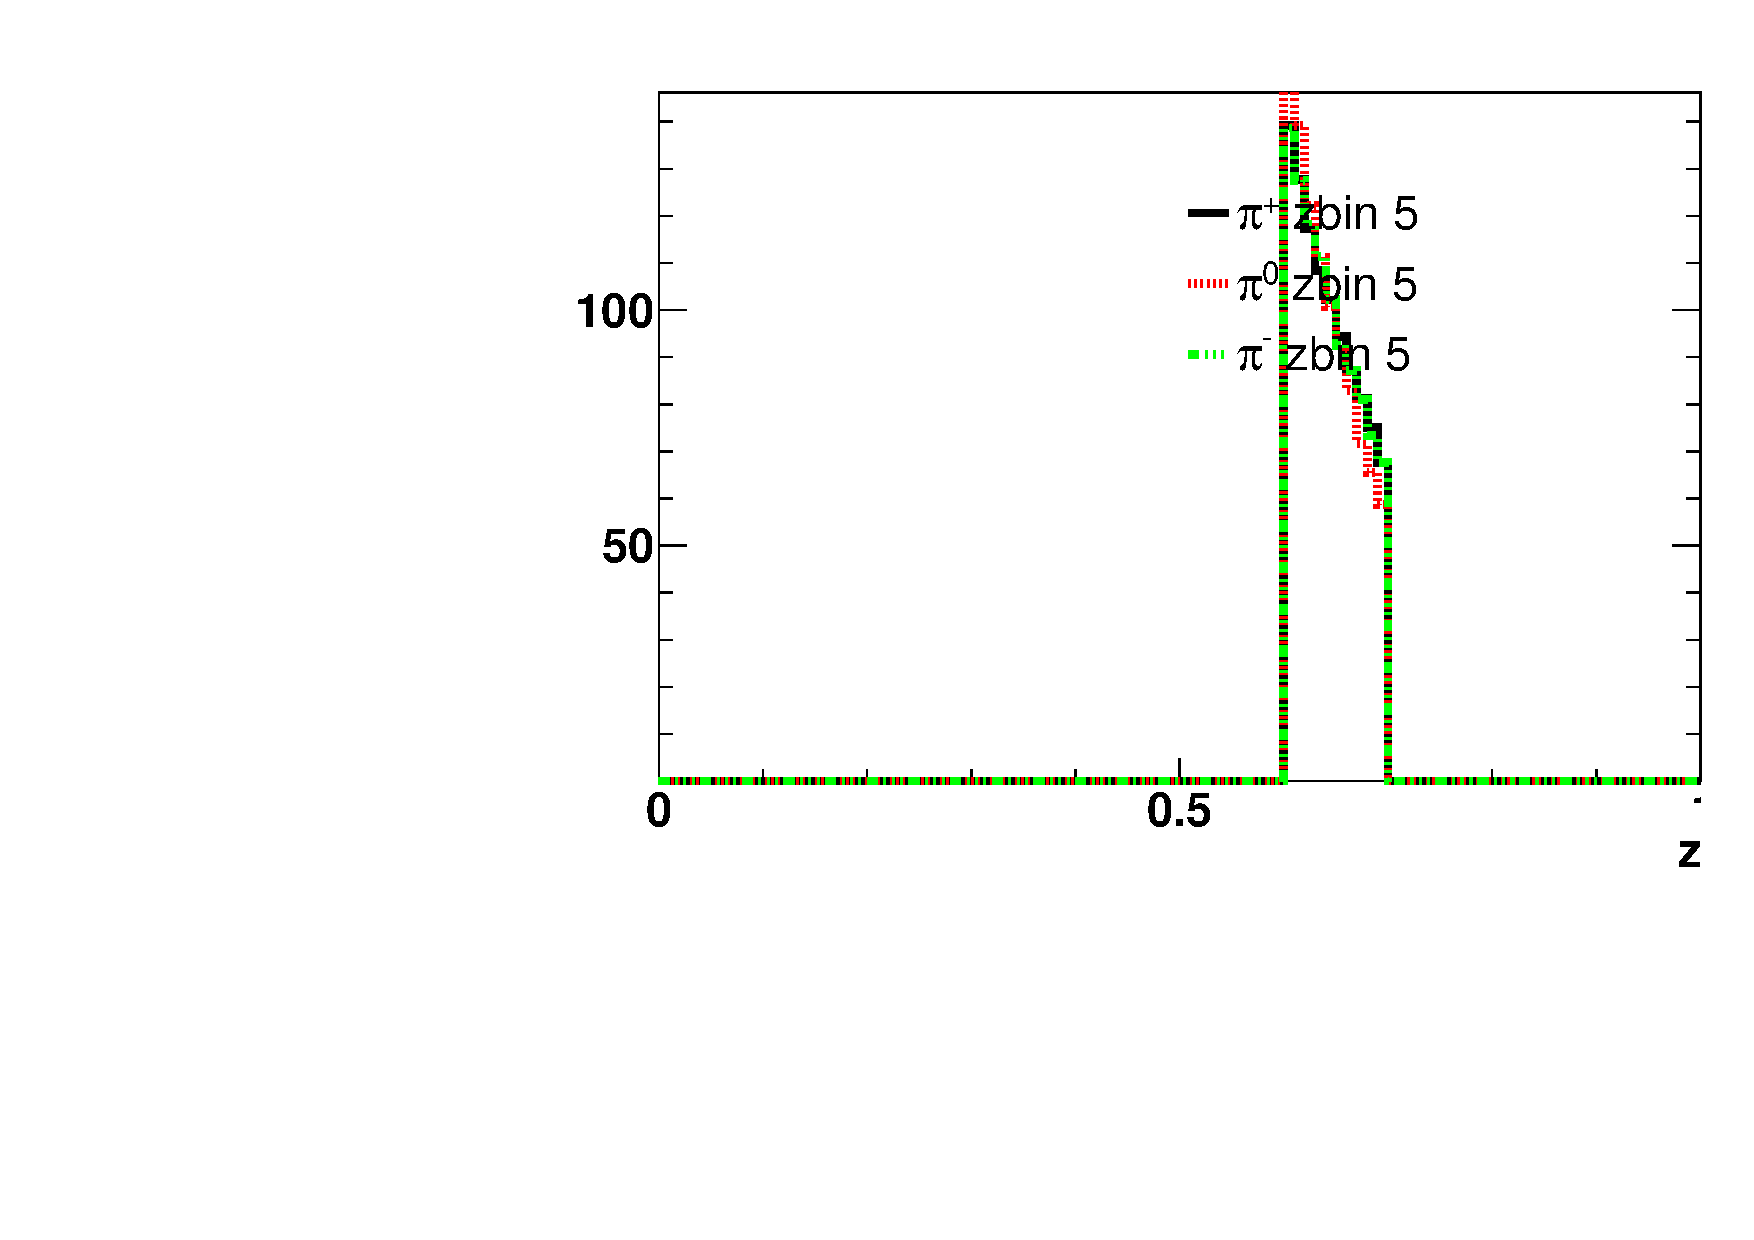
\includegraphics[width=.27\textwidth,natwidth=250,natheight=100]{figure_fiducial/had0.4/Z_distri_for_zbin_5_norm_had04.pdf}\hfill
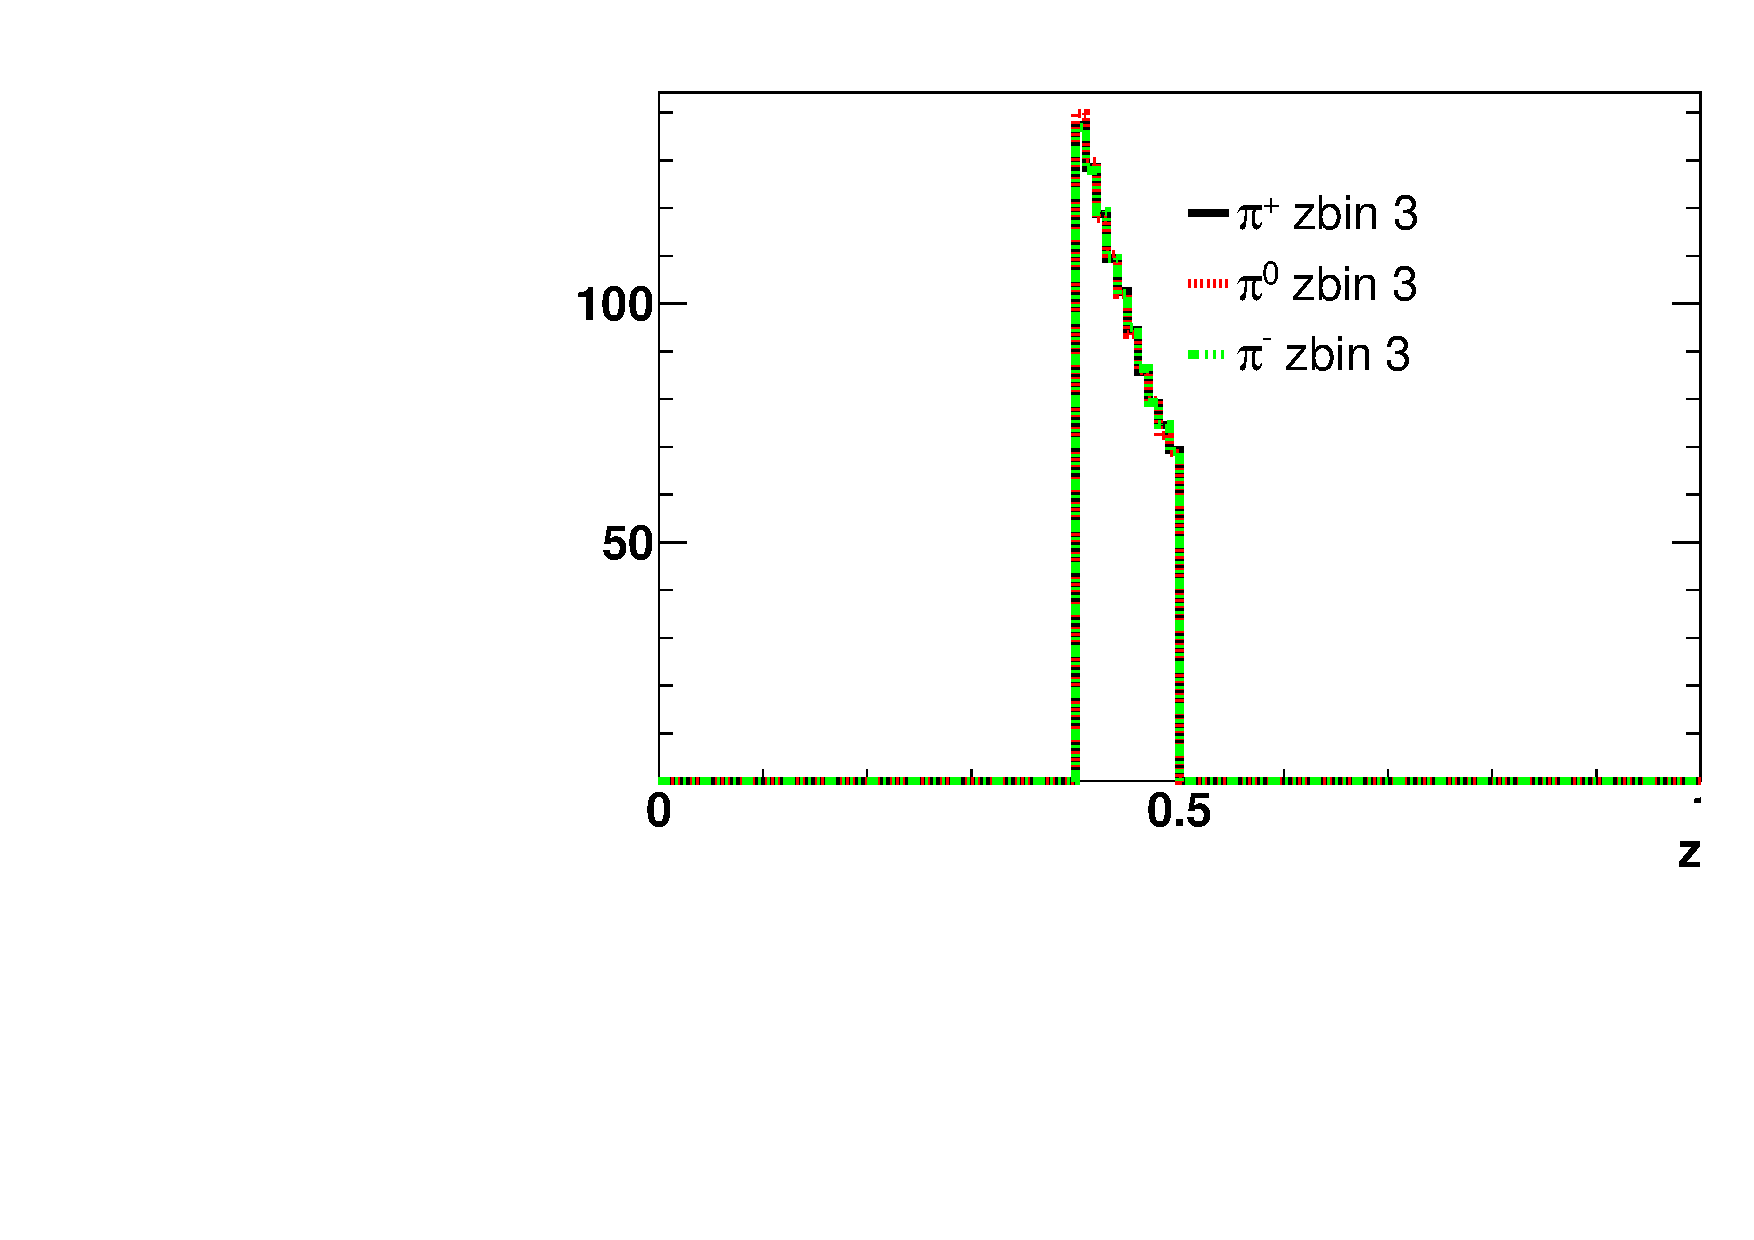
\includegraphics[width=.27\textwidth,natwidth=250,natheight=100]{figure_fiducial/had0.5/Z_distri_for_zbin_3_norm_had05.pdf}
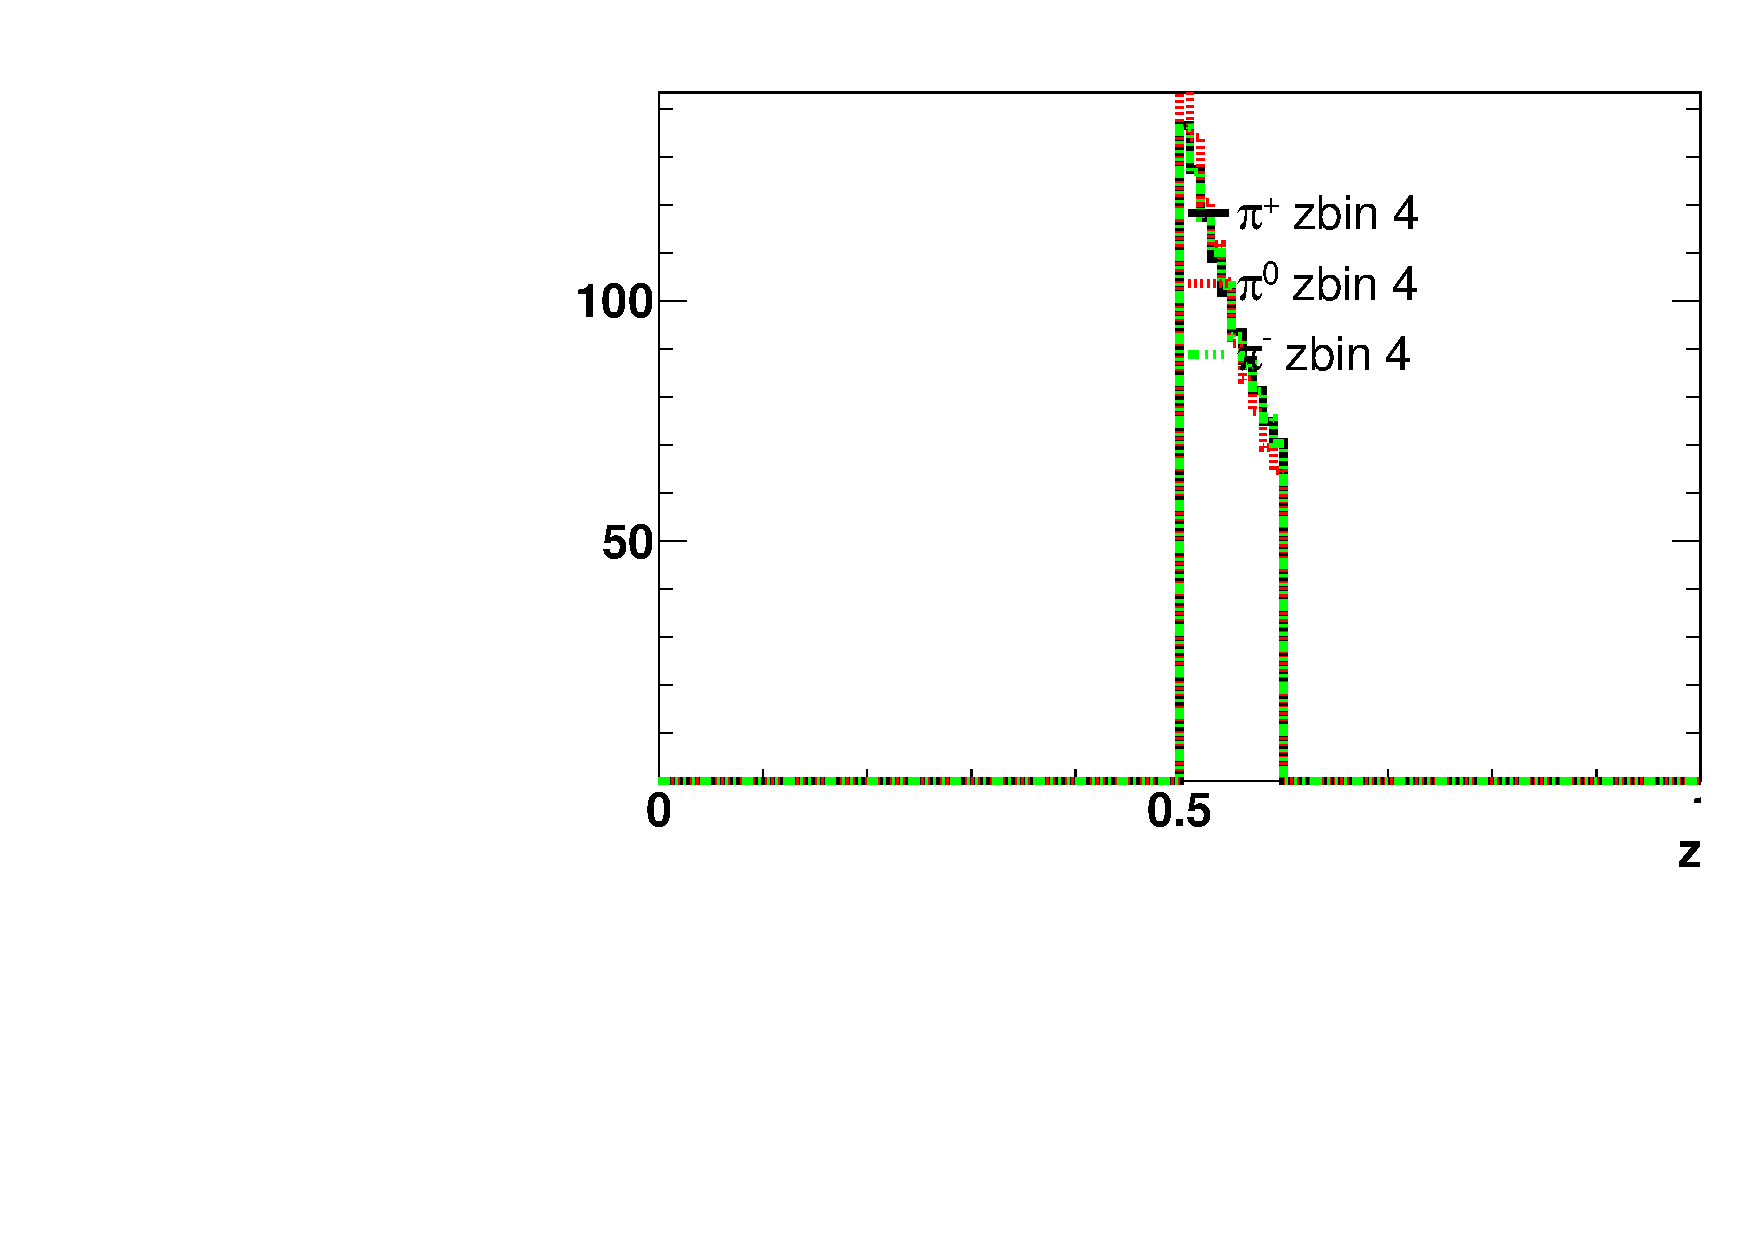
\includegraphics[width=.27\textwidth,natwidth=250,natheight=100]{figure_fiducial/had0.5/Z_distri_for_zbin_4_norm_had05.pdf}
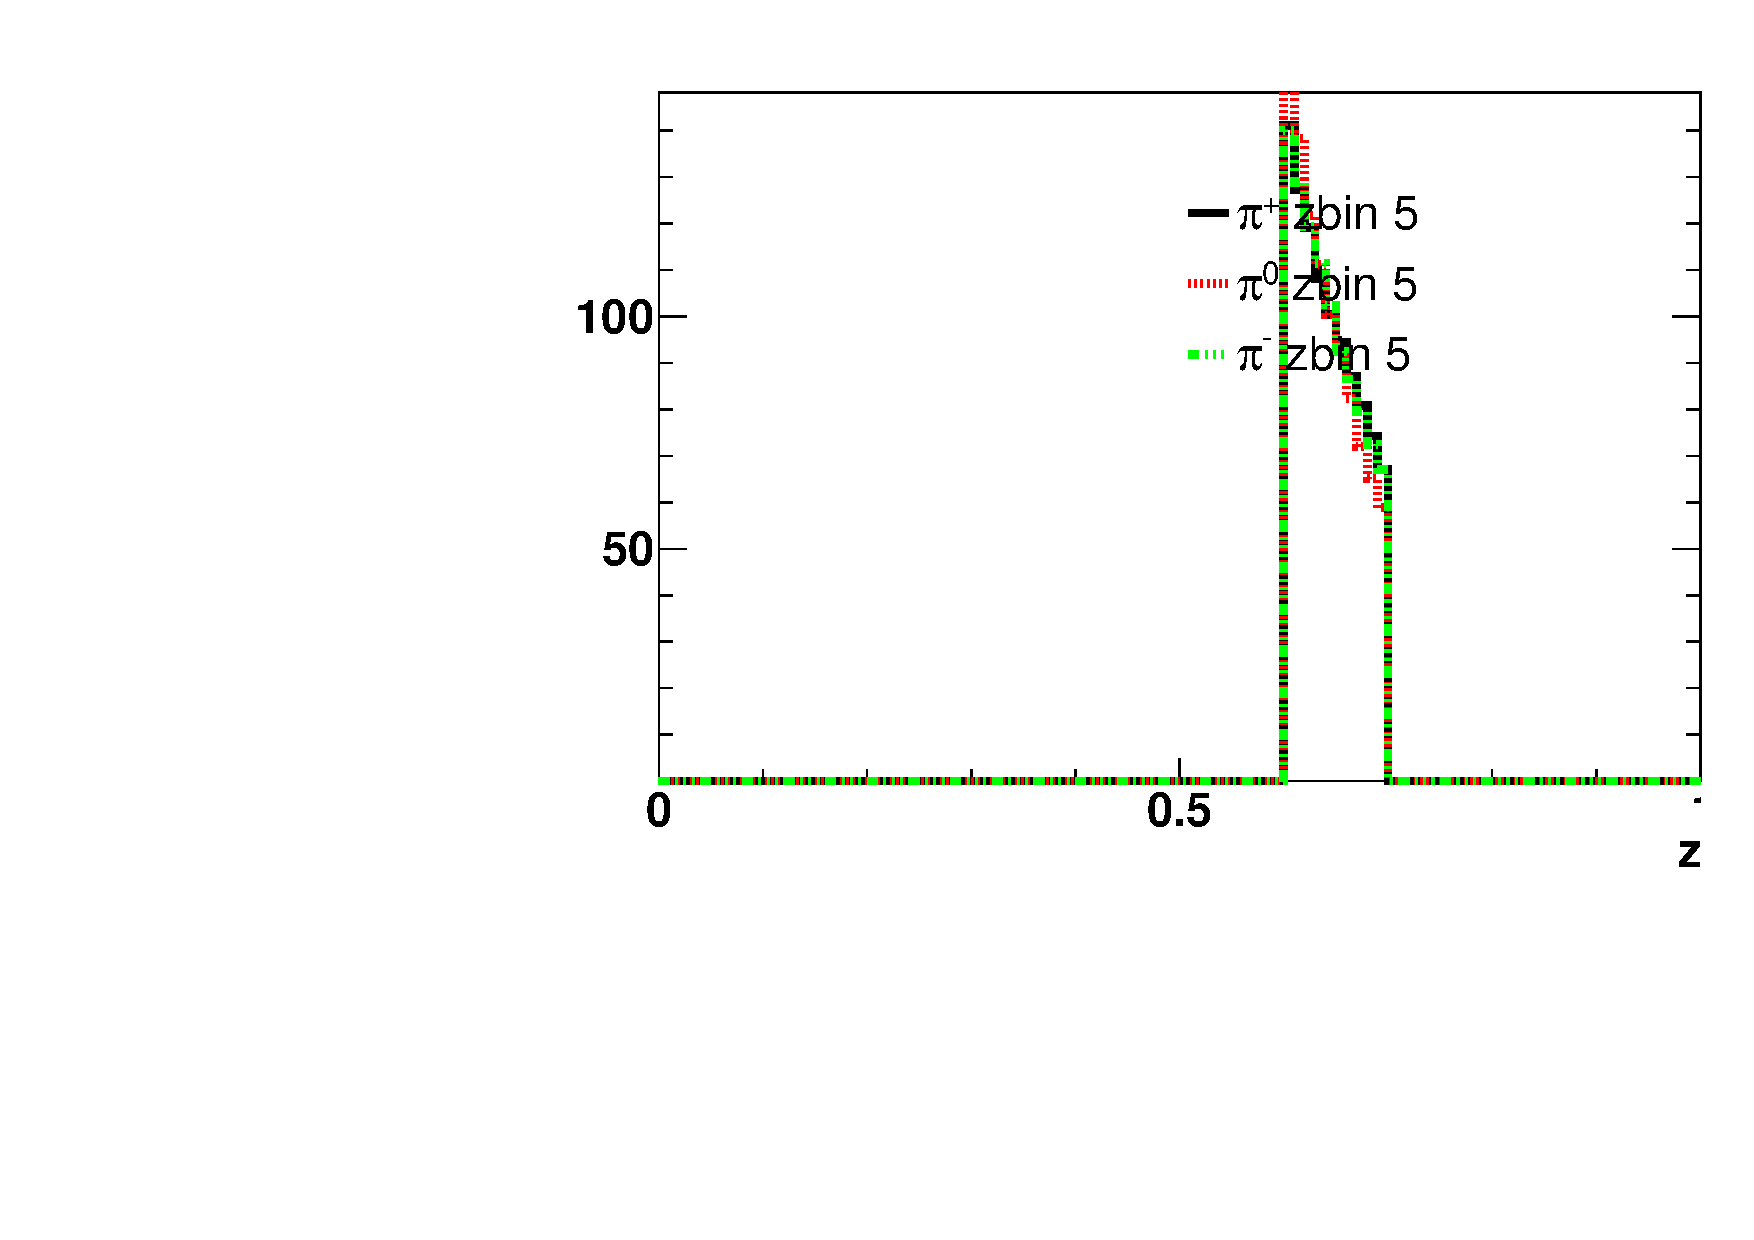
\includegraphics[width=.27\textwidth,natwidth=250,natheight=100]{figure_fiducial/had0.5/Z_distri_for_zbin_5_norm_had05.pdf}\hfill
\caption[$z$ distribution for pions in the various $z$ bins]{$z$ distribution for pions in the various $z$ bins. Hadron-direction constraint for the first and fourth row is $H_{OA}<0.3$, second and fifth row is $H_{OA}<0.4$, third and the last row is $H_{OA}<0.5$.}
\end{figure}

\begin{figure}[H]
\captionsetup[subfloat]{farskip=2pt,captionskip=1pt}
\centering
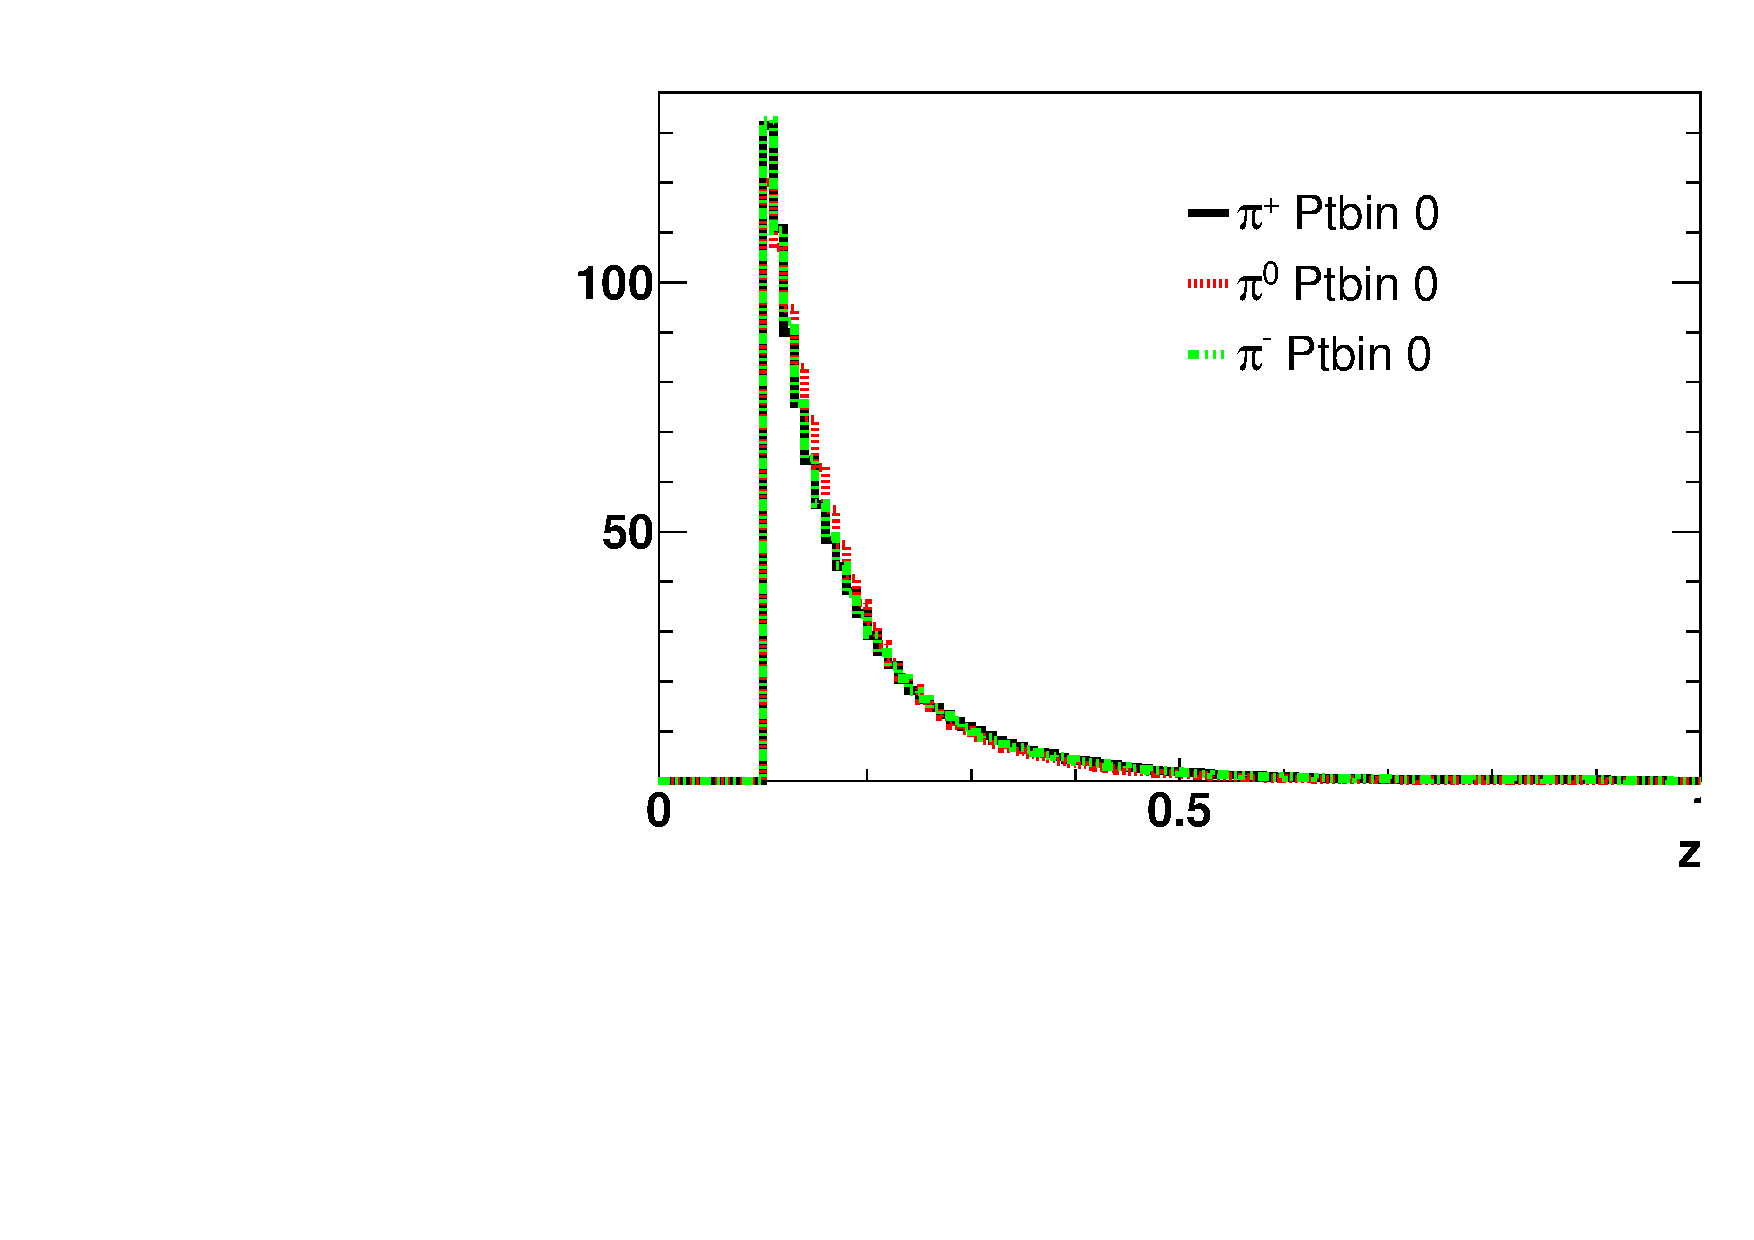
\includegraphics[width=.24\textwidth,natwidth=250,natheight=100]{figure_fiducial/had0.3/Z_distri_for_ptbin_0_norm_had03.pdf}
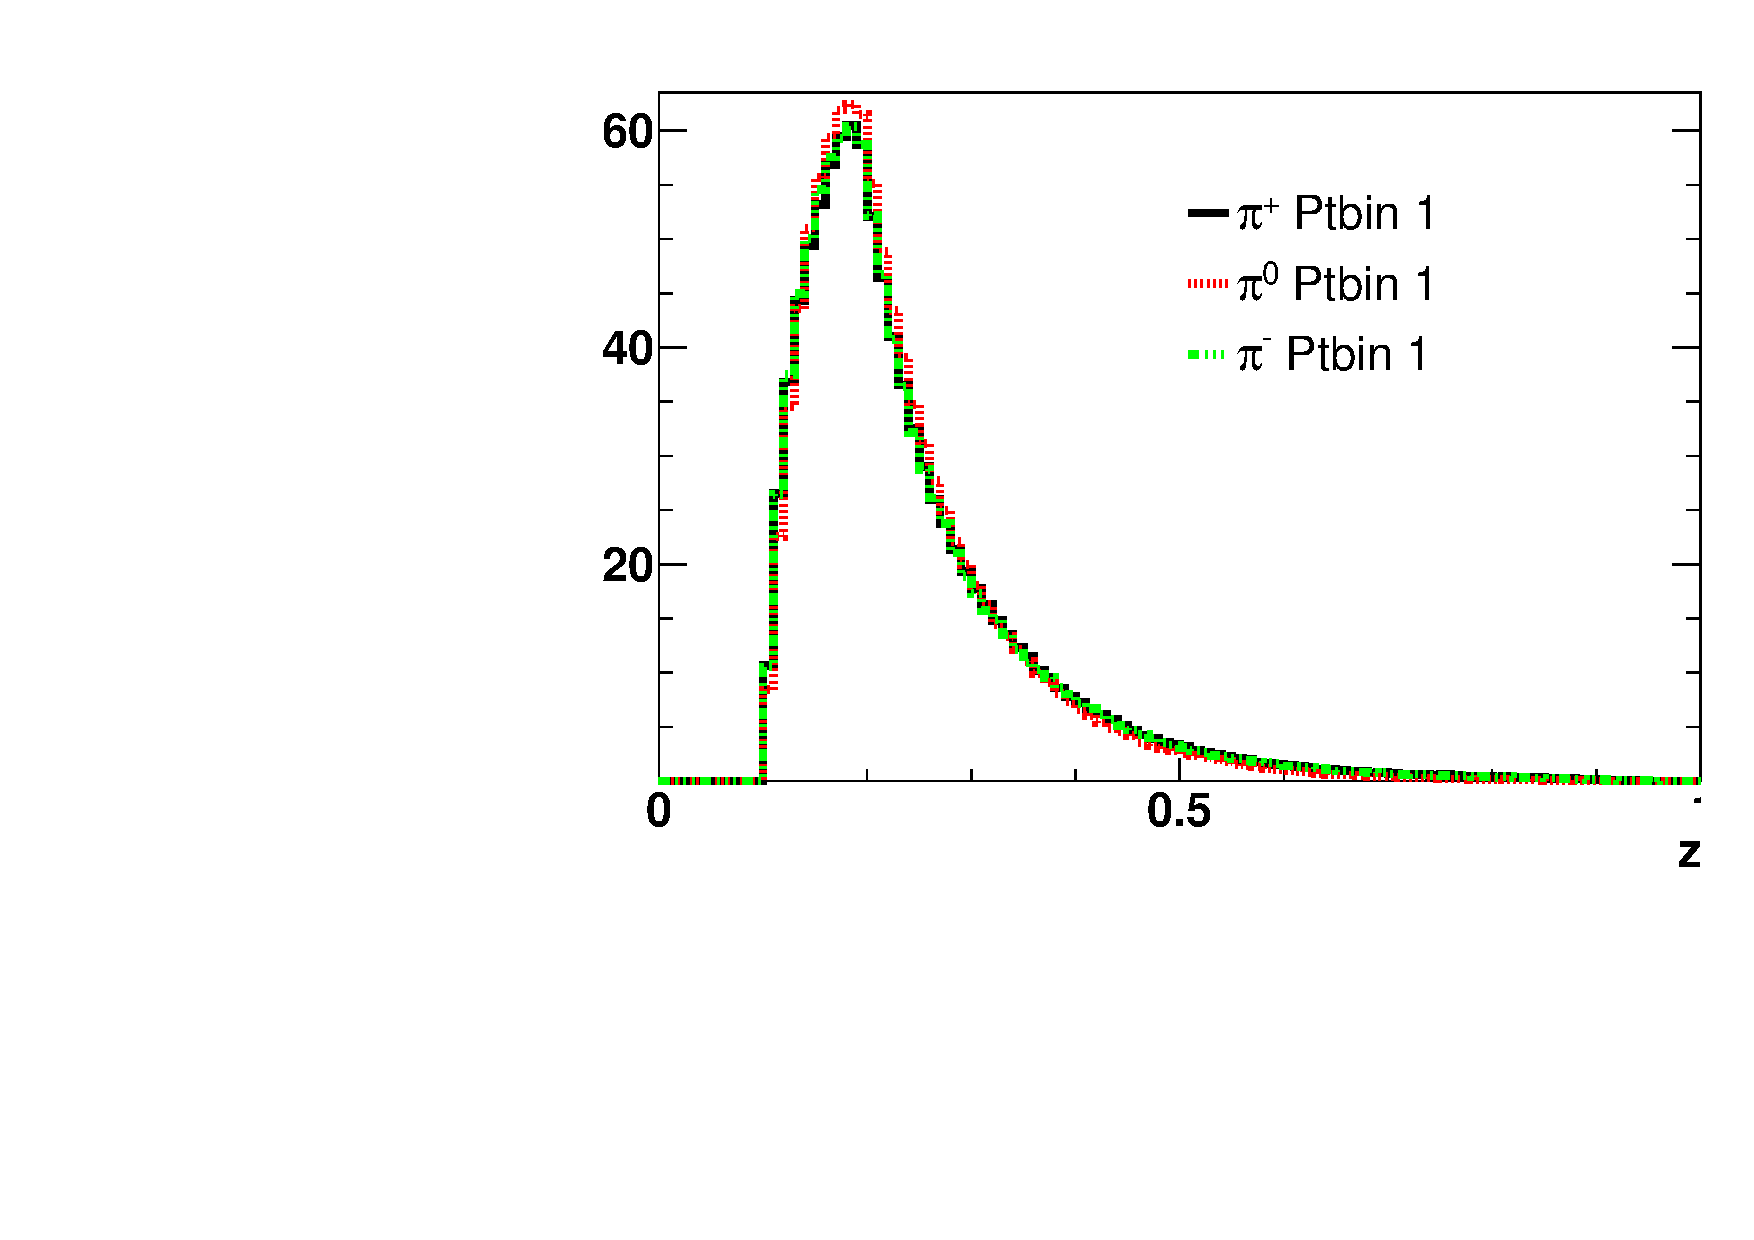
\includegraphics[width=.24\textwidth,natwidth=250,natheight=100]{figure_fiducial/had0.3/Z_distri_for_ptbin_1_norm_had03.pdf}
\includegraphics[width=.24\textwidth,natwidth=250,natheight=100]{figure_fiducial/had0.3/Z_distri_for_ptbin_2_norm_had03.pdf}
\includegraphics[width=.24\textwidth,natwidth=250,natheight=100]{figure_fiducial/had0.3/Z_distri_for_ptbin_3_norm_had03.pdf}\hfill
\includegraphics[width=.24\textwidth,natwidth=250,natheight=100]{figure_fiducial/had0.4/Z_distri_for_ptbin_0_norm_had04.pdf}
\includegraphics[width=.24\textwidth,natwidth=250,natheight=100]{figure_fiducial/had0.4/Z_distri_for_ptbin_1_norm_had04.pdf}
\includegraphics[width=.24\textwidth,natwidth=250,natheight=100]{figure_fiducial/had0.4/Z_distri_for_ptbin_2_norm_had04.pdf}
\includegraphics[width=.24\textwidth,natwidth=250,natheight=100]{figure_fiducial/had0.4/Z_distri_for_ptbin_3_norm_had04.pdf}\hfill
\includegraphics[width=.24\textwidth,natwidth=250,natheight=100]{figure_fiducial/had0.5/Z_distri_for_ptbin_0_norm_had05.pdf}
\includegraphics[width=.24\textwidth,natwidth=250,natheight=100]{figure_fiducial/had0.5/Z_distri_for_ptbin_1_norm_had05.pdf}
\includegraphics[width=.24\textwidth,natwidth=250,natheight=100]{figure_fiducial/had0.5/Z_distri_for_ptbin_2_norm_had05.pdf}
\includegraphics[width=.24\textwidth,natwidth=250,natheight=100]{figure_fiducial/had0.5/Z_distri_for_ptbin_3_norm_had05.pdf}\hfill
\caption[$z$ distribution for pions in the various $P_t$ bins]{$z$ distribution for pions in the various $P_t$ bins. Hadron-direction constraint for the first row is $H_{OA}<0.3$, second row is $H_{OA}<0.4$ and the last row is $H_{OA}<0.5$.}
\end{figure}

\subsubsection{\texorpdfstring{Kinematic Distributions of $\eta$}{Kinematic Distributions of eta}}
\label{sec:kinedistri_eta}

\begin{figure}[H]
\captionsetup[subfloat]{farskip=2pt,captionskip=1pt}
\centering
\includegraphics[width=.27\textwidth,natwidth=250,natheight=100]{figure_fiducial/had0.3_z0.3/Pt_distri_for_zbin_2_norm_had03z03.pdf}
\includegraphics[width=.27\textwidth,natwidth=250,natheight=100]{figure_fiducial/had0.3_z0.3/Pt_distri_for_zbin_3_norm_had03z03.pdf}
\includegraphics[width=.27\textwidth,natwidth=250,natheight=100]{figure_fiducial/had0.3_z0.3/Pt_distri_for_zbin_4_norm_had03z03.pdf}\hfill
\includegraphics[width=.27\textwidth,natwidth=250,natheight=100]{figure_fiducial/had0.4_z0.3/Pt_distri_for_zbin_2_norm_had04z03.pdf}
\includegraphics[width=.27\textwidth,natwidth=250,natheight=100]{figure_fiducial/had0.4_z0.3/Pt_distri_for_zbin_3_norm_had04z03.pdf}
\includegraphics[width=.27\textwidth,natwidth=250,natheight=100]{figure_fiducial/had0.4_z0.3/Pt_distri_for_zbin_4_norm_had04z03.pdf}\hfill
\includegraphics[width=.27\textwidth,natwidth=250,natheight=100]{figure_fiducial/had0.3_z0.3/Pt_distri_for_zbin_5_norm_had03z03.pdf}
\includegraphics[width=.27\textwidth,natwidth=250,natheight=100]{figure_fiducial/had0.3_z0.3/Pt_distri_for_zbin_6_norm_had03z03.pdf}\hfill\\
\includegraphics[width=.27\textwidth,natwidth=250,natheight=100]{figure_fiducial/had0.4_z0.3/Pt_distri_for_zbin_5_norm_had04z03.pdf}
\includegraphics[width=.27\textwidth,natwidth=250,natheight=100]{figure_fiducial/had0.4_z0.3/Pt_distri_for_zbin_6_norm_had04z03.pdf}\hfill
\caption[$P_t$ distributions for \(\eta\) and pions in the various $z$ bins]{$P_t$ distributions for \(\eta\) and pions in the various $z$ bins. Hadron-direction constraint for the first/third row is $H_{OA}<0.3$, second/last row is $H_{OA}<0.4$.}
\end{figure}

\begin{figure}[H]
\captionsetup[subfloat]{farskip=2pt,captionskip=1pt}
\centering
\includegraphics[width=.24\textwidth,natwidth=250,natheight=100]{figure_fiducial/had0.3_z0.3/Pt_distri_for_ptbin_0_norm_had03z03.pdf}
\includegraphics[width=.24\textwidth,natwidth=250,natheight=100]{figure_fiducial/had0.3_z0.3/Pt_distri_for_ptbin_1_norm_had03z03.pdf}
\includegraphics[width=.24\textwidth,natwidth=250,natheight=100]{figure_fiducial/had0.3_z0.3/Pt_distri_for_ptbin_2_norm_had03z03.pdf}
\includegraphics[width=.24\textwidth,natwidth=250,natheight=100]{figure_fiducial/had0.3_z0.3/Pt_distri_for_ptbin_3_norm_had03z03.pdf}\hfill
\includegraphics[width=.24\textwidth,natwidth=250,natheight=100]{figure_fiducial/had0.4_z0.3/Pt_distri_for_ptbin_0_norm_had04z03.pdf}
\includegraphics[width=.24\textwidth,natwidth=250,natheight=100]{figure_fiducial/had0.4_z0.3/Pt_distri_for_ptbin_1_norm_had04z03.pdf}
\includegraphics[width=.24\textwidth,natwidth=250,natheight=100]{figure_fiducial/had0.4_z0.3/Pt_distri_for_ptbin_2_norm_had04z03.pdf}
\includegraphics[width=.24\textwidth,natwidth=250,natheight=100]{figure_fiducial/had0.4_z0.3/Pt_distri_for_ptbin_3_norm_had04z03.pdf}\hfill
\caption[$P_t$ distributions for \(\eta\) and pions in the various $P_t$ bins]{$P_t$ distributions for \(\eta\) and pions in the various $P_t$ bins. Hadron-direction constraint for the first row is $H_{OA}<0.3$,  and  $H_{OA}<0.4$ for the second row.}
\end{figure}

\begin{figure}[H]
\captionsetup[subfloat]{farskip=2pt,captionskip=1pt}
\centering
\includegraphics[width=.27\textwidth,natwidth=250,natheight=100]{figure_fiducial/had0.3_z0.3/Z_distri_for_zbin_2_norm_had03z03.pdf}
\includegraphics[width=.27\textwidth,natwidth=250,natheight=100]{figure_fiducial/had0.3_z0.3/Z_distri_for_zbin_3_norm_had03z03.pdf}
\includegraphics[width=.27\textwidth,natwidth=250,natheight=100]{figure_fiducial/had0.3_z0.3/Z_distri_for_zbin_4_norm_had03z03.pdf}\hfill
\includegraphics[width=.27\textwidth,natwidth=250,natheight=100]{figure_fiducial/had0.4_z0.3/Z_distri_for_zbin_2_norm_had04z03.pdf}
\includegraphics[width=.27\textwidth,natwidth=250,natheight=100]{figure_fiducial/had0.4_z0.3/Z_distri_for_zbin_3_norm_had04z03.pdf}
\includegraphics[width=.27\textwidth,natwidth=250,natheight=100]{figure_fiducial/had0.4_z0.3/Z_distri_for_zbin_4_norm_had04z03.pdf}\hfill
\includegraphics[width=.27\textwidth,natwidth=250,natheight=100]{figure_fiducial/had0.3_z0.3/Z_distri_for_zbin_5_norm_had03z03.pdf}
\includegraphics[width=.27\textwidth,natwidth=250,natheight=100]{figure_fiducial/had0.3_z0.3/Z_distri_for_zbin_6_norm_had03z03.pdf}\hfill\\
\includegraphics[width=.27\textwidth,natwidth=250,natheight=100]{figure_fiducial/had0.4_z0.3/Z_distri_for_zbin_5_norm_had04z03.pdf}
\includegraphics[width=.27\textwidth,natwidth=250,natheight=100]{figure_fiducial/had0.4_z0.3/Z_distri_for_zbin_6_norm_had04z03.pdf}\hfill
\caption[$z$ distributions for \(\eta\) and pions in the various $z$ bins]{$z$ distributions for \(\eta\) and pions in the various $z$ bins. Hadron-direction constraint of the first/third row is $H_{OA}<0.3$, second/fourth row is $H_{OA}<0.4$.}
\end{figure}

\begin{figure}[H]
\captionsetup[subfloat]{farskip=2pt,captionskip=1pt}
\centering
\includegraphics[width=.24\textwidth,natwidth=250,natheight=100]{figure_fiducial/had0.3_z0.3/Z_distri_for_ptbin_0_norm_had03.pdf}
\includegraphics[width=.24\textwidth,natwidth=250,natheight=100]{figure_fiducial/had0.3_z0.3/Z_distri_for_ptbin_1_norm_had03.pdf}
\includegraphics[width=.24\textwidth,natwidth=250,natheight=100]{figure_fiducial/had0.3_z0.3/Z_distri_for_ptbin_2_norm_had03.pdf}
\includegraphics[width=.24\textwidth,natwidth=250,natheight=100]{figure_fiducial/had0.3_z0.3/Z_distri_for_ptbin_3_norm_had03.pdf}\hfill
\includegraphics[width=.24\textwidth,natwidth=250,natheight=100]{figure_fiducial/had0.4_z0.3/Z_distri_for_ptbin_0_norm_had04.pdf}
\includegraphics[width=.24\textwidth,natwidth=250,natheight=100]{figure_fiducial/had0.4_z0.3/Z_distri_for_ptbin_1_norm_had04.pdf}
\includegraphics[width=.24\textwidth,natwidth=250,natheight=100]{figure_fiducial/had0.4_z0.3/Z_distri_for_ptbin_2_norm_had04.pdf}
\includegraphics[width=.24\textwidth,natwidth=250,natheight=100]{figure_fiducial/had0.4_z0.3/Z_distri_for_ptbin_3_norm_had04.pdf}\hfill
    \caption[$z$ distributions for \(\eta\) and pions in the various $P_t$ bins]{$z$ distributions for \(\eta\) and pions in the various $P_t$ bins. Hadron-direction constraint of the first row is $H_{OA}<0.3$, and  $H_{OA}<0.4$ for the second row.}
\end{figure}